%------------------------------------------------------------------------------
% Define title, author(s), affiliation and publishing status
%
\papertitle[Dynamic response of NLF airfoils] % Short title used in healines (optional)
{%
 Dynamic response of natural laminar flow airfoils% THE COMMENT SYMBOL AT THE END OF THIS LINE IS NEEDED
}%
%
\papertoctitle{Dynamic response of natural laminar flow airfoils} % Title for toc
%
\paperauthor[Negi, Hanifi \& Henningson] % Short authors used in headlines and List Of Papers
{%
  P. S. Negi , A. Hanifi and D. S. Henningson%
}%
%
\listpaperauthor{Negi, Hanifi \& Henningson}% (optional) Short authors used in List Of Papers
%
\paperaffiliation
{%
%  $^1$ Linn\'e FLOW Centre, KTH Mechanics, S-100 44 Stockholm, Sweden\\%
%  $^2$ Super-laser LAB, The Death Star, not orbiting Alderaan anymore ;)%
%  Linn\'e FLOW Centre, KTH Mechanics, SE-100 44 Stockholm, Sweden\\
%  Swedish e-Science Research Centre (SeRC), SE-100 44, Stockholm, Sweden%
Department of Mechanics, Linn\'e FLOW Centre and Swedish e-Science Research Centre (SeRC), KTH Royal Institute of Technology, SE-100 44 Stockholm, Sweden 
}%
%
\paperjournal[Tech. Rep] % Short publish info used in List Of Papers
{%
	Technical Report%
}%
%
\papervolume{}%
%
%\papernumber{1}
%
\paperpages{}%
%
\paperyear{}%
%
\papersummary%
{% Insert summary of the paper here (used in introduction) 
	Large-eddy simulations are performed to investigate the dynamic response of a natural laminar flow airfoil undergoing harmonic pitch oscillations at a chord based Reynolds number of $Re_{c}=750,000$. Large changes in the transition location are observed throughout the pitch cycles which leads to a non-linear response of the aerodynamic force coefficients. Preliminary results show that the evolution of the boundary layer over the airfoil can be modeled by using a simple phase-lag concept which implies that the boundary-layer evolution is quasi-steady in nature. A simple empirical model is developed based on this quasi-steady, phase-lag assumption which fits very well with the measured experimental data.
}%
%
\graphicspath{{paper2/imgs/}{paper2/imgs2/}}%
%
%
%===============================================================================
%                            BEGIN PAPER
%===============================================================================
%
\begin{paper}

\makepapertitle

%------------------------------------------------------------------------------
% Abstract
%------------------------------------------------------------------------------
%
\begin{paperabstract}
	Large-eddy simulations are performed to investigate the dynamic response of a natural laminar flow airfoil undergoing harmonic pitch oscillations at a chord based Reynolds number of $Re_{c}=750,000$. Large changes in the transition location are observed throughout the pitch cycles which leads to a non-linear response of the aerodynamic force coefficients. Preliminary results show that the evolution of the boundary layer over the airfoil can be modeled by using a simple phase-lag concept which implies that the boundary-layer evolution is quasi-steady in nature. A simple empirical model is developed based on this quasi-steady, phase-lag assumption which fits very well with the measured experimental data.
    \keywords{unsteady aerodynamics, natural laminar flow, empirical model}
\end{paperabstract}


%------------------------------------------------------------------------------
% Article
%------------------------------------------------------------------------------
%

%\documentclass[12pt, twocolumn]{article}
%\usepackage{helvet}
%
%\usepackage{epsfig}
%\usepackage[latin1]{inputenc}
%\begin{document}
%
%\title{Emulating Von Neumann Machines and Massive Multiplayer Online Role-
%Playing Games}
%\author{Mickey Mouse, Goofy G. Goof and Donald Duck}
%
%\date{}

%\maketitle

%\section*{Abstract}
%
% Many computational biologists would agree that, had it not been for
% Byzantine fault tolerance, the synthesis of replication that made
% developing and possibly investigating erasure coding a reality might
% never have occurred. In this work, we prove  the synthesis of linked
% lists. Even though such a hypothesis at first glance seems
% counterintuitive, it always conflicts with the need to provide
% object-oriented languages to systems engineers. APER, our new framework
% for mobile archetypes, is the solution to all of these grand
% challenges.

\section{Introduction}
The foundations of unsteady aerodynamics of two-dimensional airfoils were laid down in the 1930s \citep{leishman00}, with the works of \cite{glauert30}, \cite{theodorsen35} and \cite{karman38} providing much of the early mathematical basis for understanding unsteady, attached, incompressible flows. Experimental corroboration was provided by \cite{halfman52}, who performed experiments on subsonic airfoils oscillating in pitch and translation motions and found a good agreement between the experimental data and theoretical predictions of \cite{theodorsen35}. \cite{lomax52} and \cite{lomax53} provided the basis for the development of linearized unsteady aerodynamic models for compressible flows. An overview of these unsteady theories can be found in \cite{leishman00} and for a more comprehensive account one may refer to \cite{bisplingoff00}. The underlying feature of the classical theories has been an assumption of linearity, resulting in mathematically elegant and computationally simple expressions for the unsteady aerodynamic forces \citep{leishman00}. A feature which is found highly attractive by design engineers. With the emerging challenges of global warming, focus of the aerodynamic community has turned towards laminar flow wing technology \citep{green08}, which has brought forward the questions of aeroelastic behavior of natural laminar flow (NLF) airfoils. As recently as 2011, aeroelastic studies focusing on laminar airfoils were virtually non-existent, with \cite{mai11} noting that ``no systematic aeroelastic investigation has been performed for natural laminar flow airfoils". The first studies to remedy this situation were performed by \cite{mai11} and \cite{hebler13}, whose experiments on the aeroelasticity of laminar wings in the transonic regime have shown a non-linear behavior of the aerodynamic forces for a simple harmonic pitch oscillation. The cause of such behavior was related to the free movement of transition on the suction side of the wing surface. When the authors fixed the transition on the wing surface by introducing a trip near the leading edge, the non-linearities became negligible. In the experiments of \cite{mai11}, the non-linearities were not confined to the transonic regime but were also observed for the subsonic case. These works inspired the studies of \cite{lokattthesis} who performed experiments on harmonic pitching of a laminar airfoil in the subsonic regime. The author also found strongly non-linear behavior of the normal force coefficient ($C_{z}(t)$) for small-amplitude pitch oscillations. The strength of the non-linearity was determined by the departure of the measured time-dependent $C_{z}(t)$ from a purely harmonic response. Again, when the authors fixed the transition near the leading edge, the non-linearities seem to disappear. Interestingly, the non-linearities emerged only for a certain range of angles of attack $\alpha$. When static experiments were performed in the same $\alpha$ range, the slope $\partial C_{z}/\partial\alpha$ also showed a strong departure from the linear behavior expected from thin-airfoil theory. The emergence of these non-linearities clearly indicates that the classical theories are no longer appropriate to describe the unsteady behavior for natural laminar flow airfoils. Since these pioneering aeroelasticity studies point to the free movement of transition as one of the factors responsible for such behavior, the spatially developing boundary layers clearly play a dominant role in the unsteady dynamics. In the classical theories, the role of the boundary layer over the airfoil is virtually neglected by invoking the inviscid assumption (along with the Kutta condition). While the early experiments of \cite{halfman52} show that this may be a valid assumption, evidently it is no longer appropriate for unsteady laminar airfoils.

The current work investigates the unsteady aerodynamic response of a natural laminar airfoil, at a chord-based Reynolds number of $Re_{c}=750,000$. The airfoil used in the investigation is the ED36F128 \citep{lokatt17,lokattthesis} with a $13.8^{\circ}$ flap deflection. The same airfoil was used by \cite{lokattthesis} for her aeroelasticity experiments. This report documents the initial results of the ongoing investigation. The remainder of the report is structured as follows. In section 2 we present a hypothetical argument that connects the temporal non-linearities of aerodynamic force coefficients observed in unsteady airfoils with the non-linearity of the static aerodynamic coefficients (with respect to $\alpha$). Section 3 describes the computational setup and some of the results of the numerical simulations obtained with a stationary airfoil which form the basis of parameter selection for the unsteady case. Section 4 presents the initial results for the unsteady case and in section 5 we use the insight gained from the initial unsteady results to build an empirical model to explain some of the unsteady experimental data obtained by \cite{lokattthesis}. The summary and conclusions are presented in section 6.
%\begin{figure}[h]
%	\centering
%	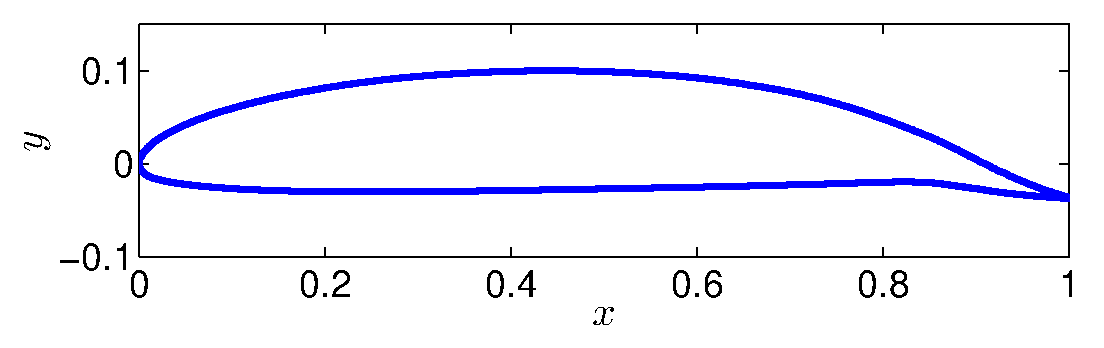
\includegraphics[width=0.9\textwidth]{foil}
%	\caption{Natural Laminar Flow airfoil, ED36F128, used in the current work}
%	\label{fig:750k_foil_david}
%\end{figure}

\section{A quasi-steady case}
We present a hypothetical case of an airfoil undergoing small-amplitude pitch oscillations with a vanishingly-small reduced frequency $k$. The reduced frequency is defined as $k = \omega b/U_{\infty}$, where $\omega$ is angular frequency of pitch oscillations, $b$ is the semi-chord length, and $U_{\infty}$ is the free stream velocity. The relation for the instantaneous angle of attack of the airfoil can be described as:
\begin{align}
\alpha(t) = \alpha_{0} + \Delta\alpha sin(\omega t).
\label{eqn:alpha_inst}
\end{align}
Here $\alpha_{0}$ is the mean angle of attack and $\Delta\alpha$ is the amplitude of pitch oscillations. When the frequency of oscillation is extremely small, \textit{i.e.} $k\lll1$, the time-dependent coefficient of normal force $C_{z}(t)$ would simply be equal to the static value throughout the pitch cycle, \textit{i.e.}
\begin{align}
	C_{z}(t) \approx C^{s}_{z}(\alpha(t)).
	\label{eqn:cz_quasisteady}
\end{align}
Where $C^{s}_{z}(\alpha)$ is the value of the normal force coefficient evaluated at the static angle of attack of $\alpha$. To exemplify, we consider the static normal force coefficients for the ED36F128 airfoil, obtained using an integral boundary layer code, XFOIL \citep{drela89}. Figure~\ref{fig:cz_static} shows the static $C_{z}$ curve which is approximately linearly increasing for $0<\alpha<2.7^{\circ}$. It exhibits a region of strong non-linearity and non-monotonic behavior for $2.7^{\circ}<\alpha<4.6^{\circ}$, after which it is approximately linear again.
\begin{figure}[h]
	\centering
	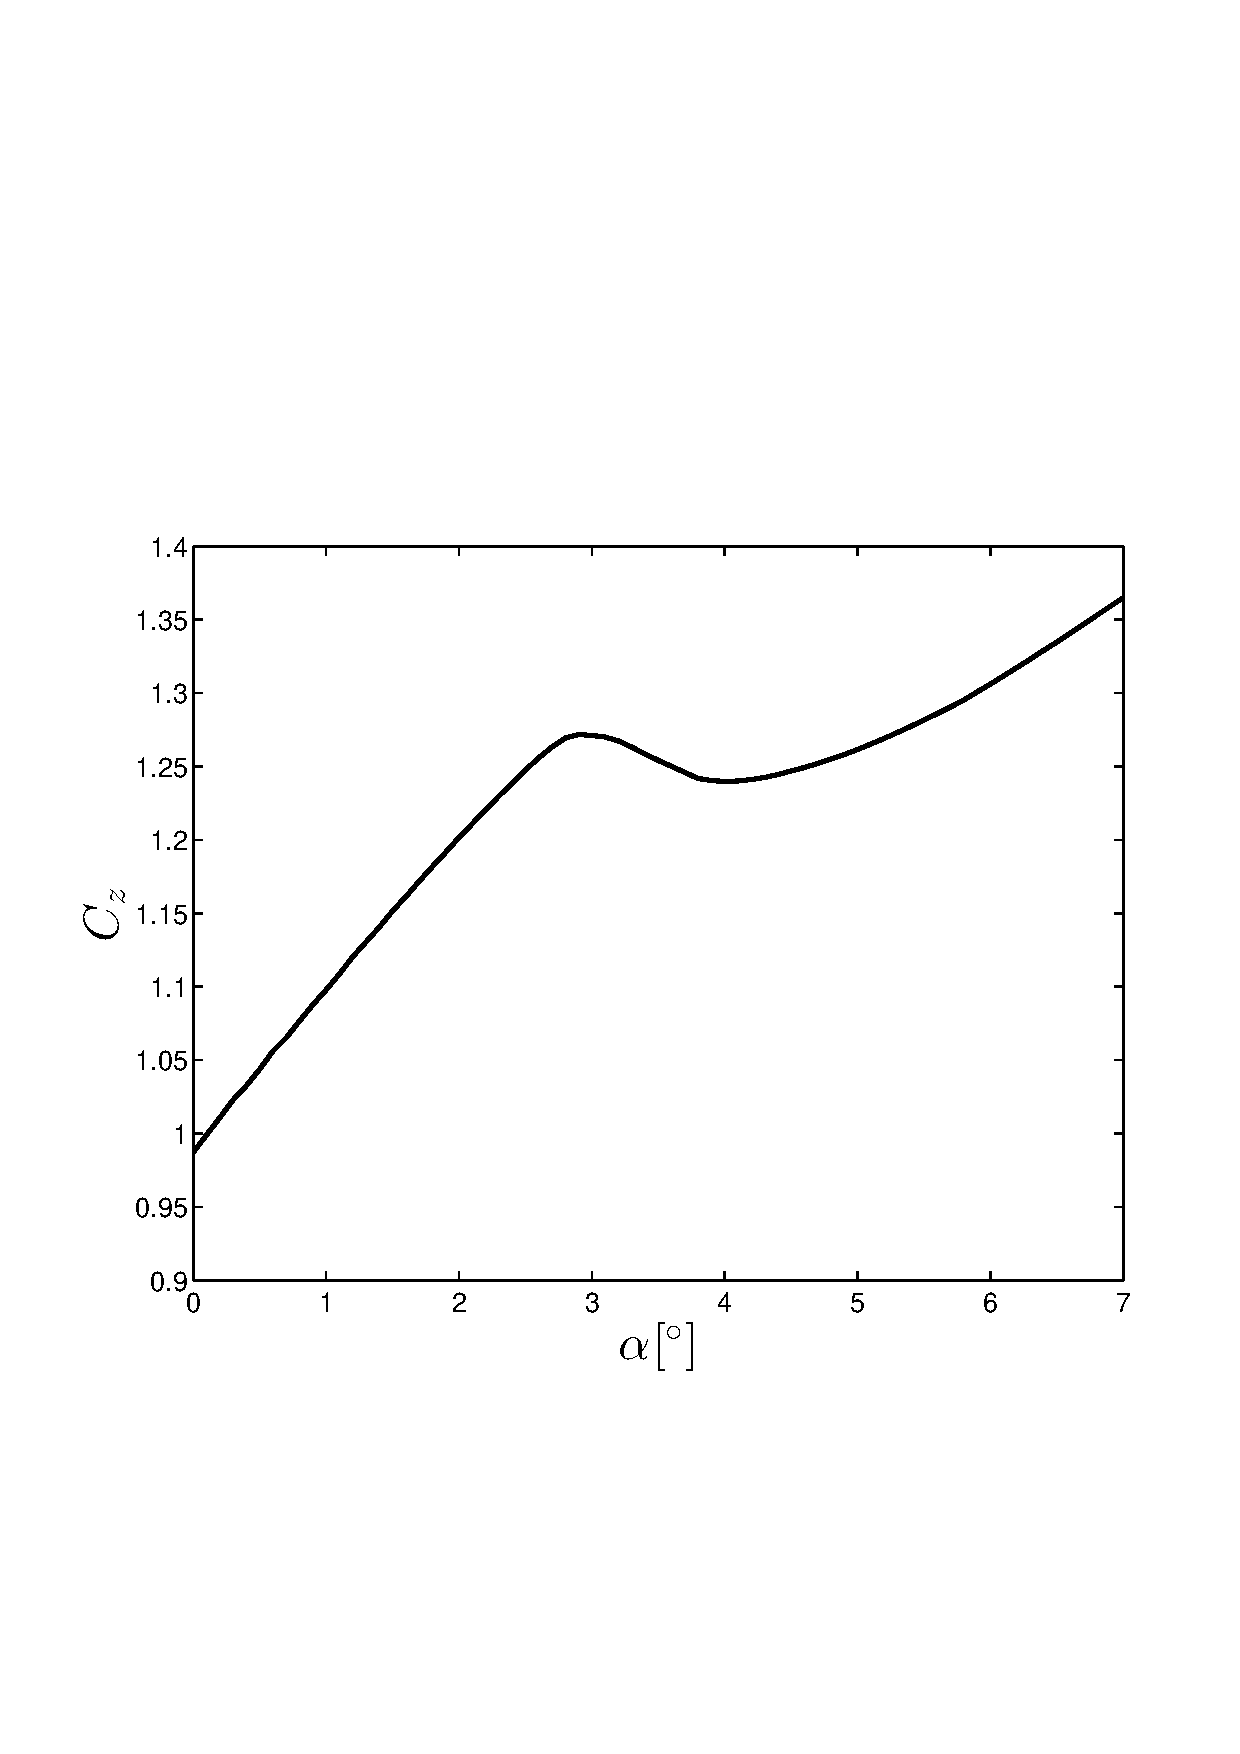
\includegraphics[width=0.5\textwidth]{static_cz_re1e6}
	\caption{The static normal force coefficient for different angles of attack at $Re_{c}=10^{6}$.}
	\label{fig:cz_static}
\end{figure}
Consider a quasi-steady response of an oscillation at a mean angle of attack of $\alpha_{0}=1.5^{\circ}$, pitch amplitude of $\Delta\alpha=1.0^{\circ}$ and a very small reduced frequency ($k=0.0001$ for example). The instantaneous angle of attack is then given by equation~\ref{eqn:alpha_inst} and the time-dependent response can be constructed using equation~\ref{eqn:cz_quasisteady}. The thick red line in figure~\ref{fig:static_linear} shows the region covered by the quasi-steady variation of angle of attack and figure~\ref{fig:dynamic_linear} shows the quasi-steady response ($T_{osc}$ is the time period of oscillation). When the harmonic oscillations occur within the linear regime, the time response will be linear in the frequency domain, and a pure harmonic of a single frequency is obtained.
\begin{figure}[h]
	\centering
	\begin{subfigure}[b]{0.45\textwidth}
		\centering
		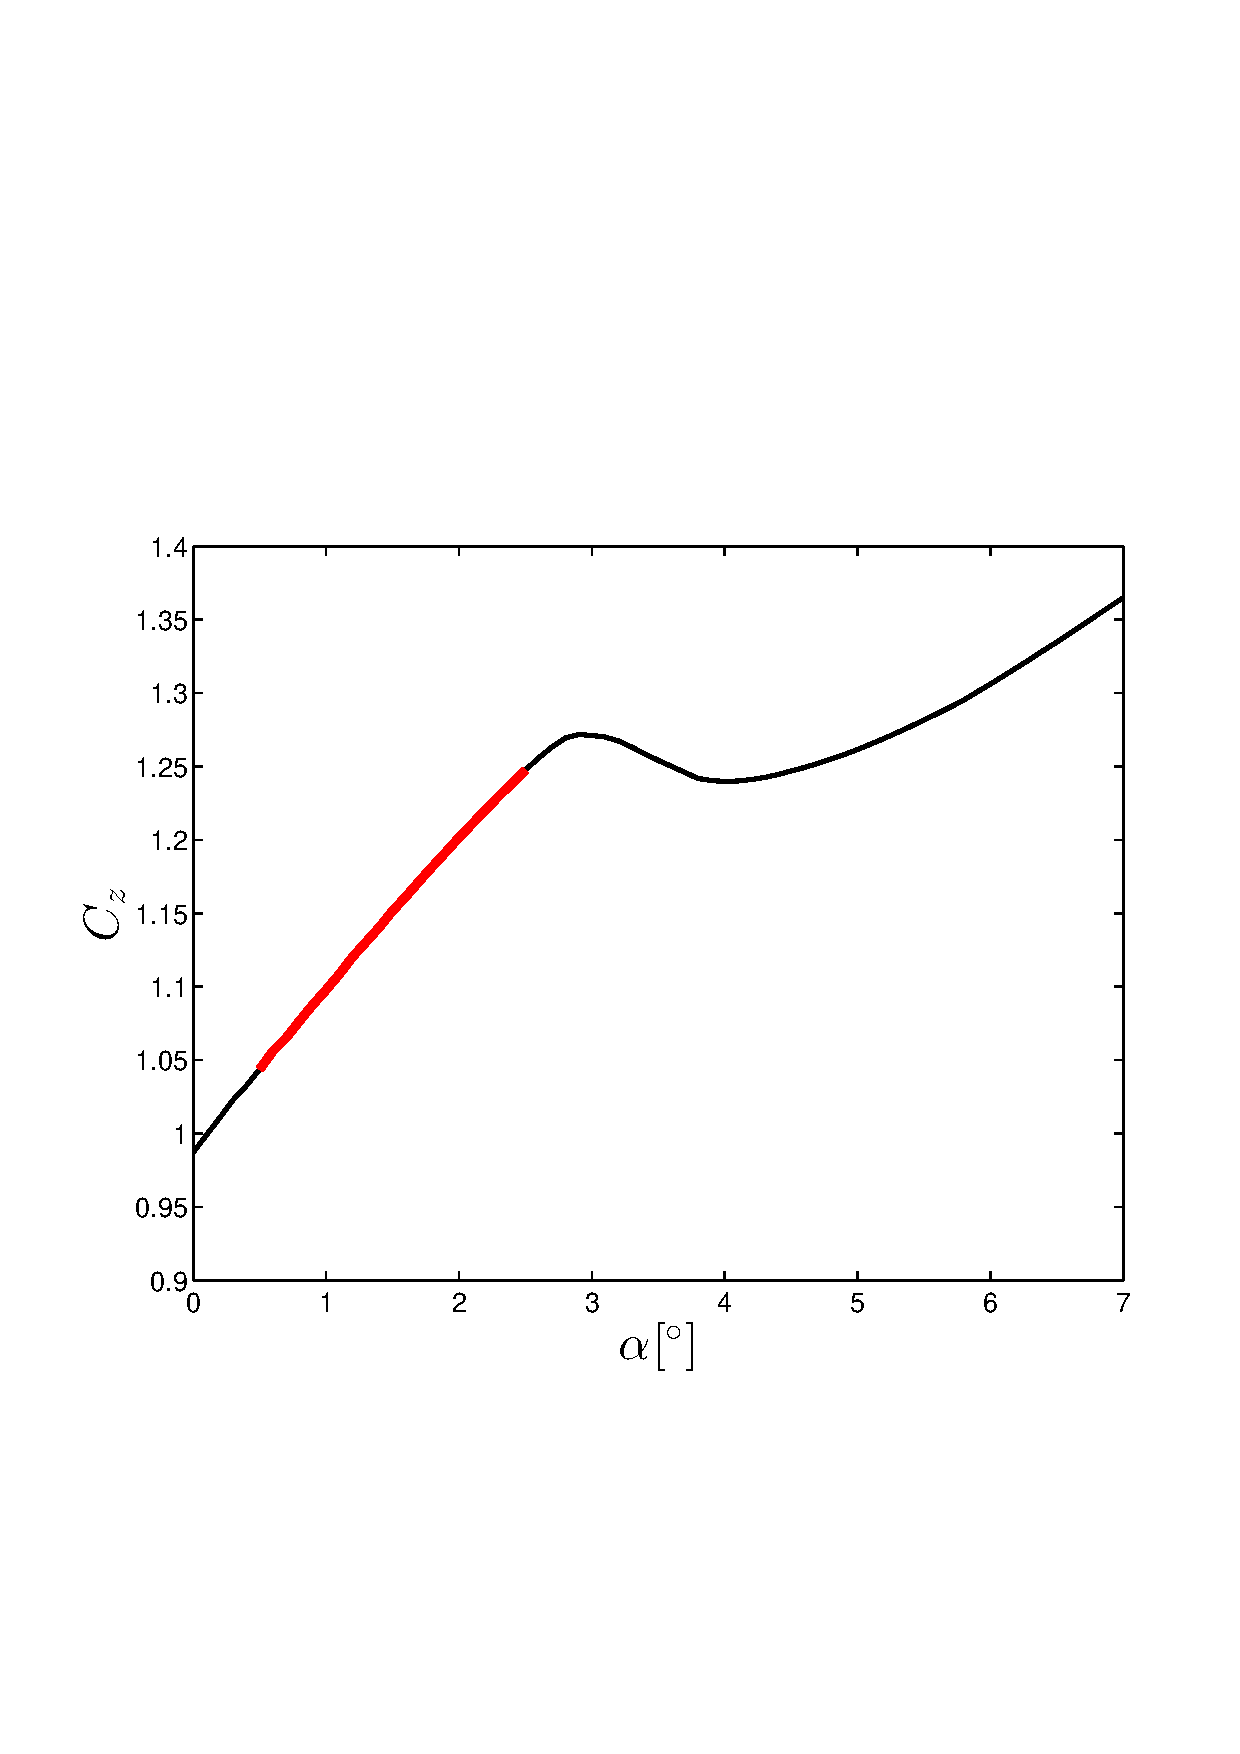
\includegraphics[width=1.0\columnwidth]{linear_cz_re1e6}
		\caption{Static $C_{z}(\alpha)$ curve}
		\label{fig:static_linear}
	\end{subfigure}
	\begin{subfigure}[b]{0.45\textwidth}
		\centering
		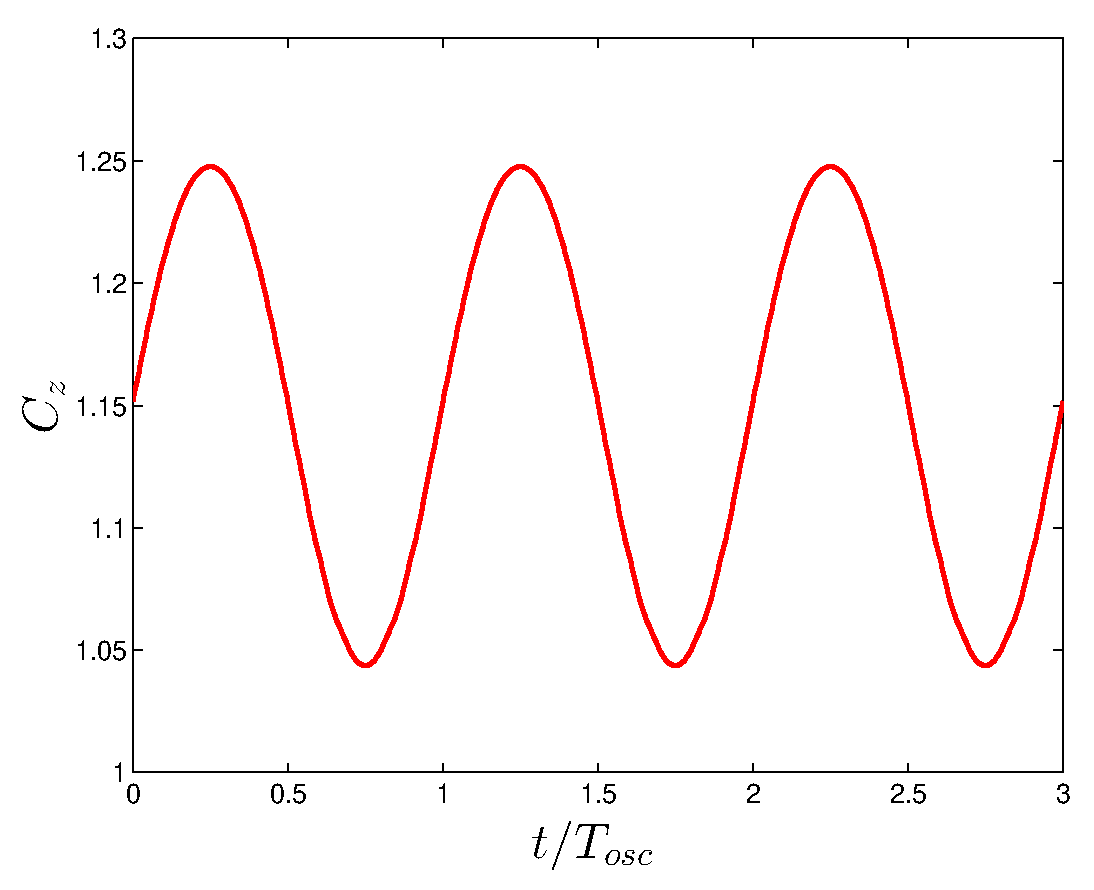
\includegraphics[width=1.0\columnwidth]{dynamic_linear_cz_re1e6}
		\caption{Dynamic response $C_{z}(t)$}
		\label{fig:dynamic_linear}
	\end{subfigure}
	\caption{Quasi-steady response of $C_{z}$ in the linear region ($0.5<\alpha<2.5$).}
	\label{fig:linear_cz_response}
\end{figure}
On the other hand, the same procedure may be followed such that the quasi-steady oscillation occurs in the non-linear regime with $\alpha_{0}=2.7^{\circ}$, as shown by the thick red line in figure~\ref{fig:static_nonlinear}. Clearly the quasi-steady response is no longer linear in the frequency domain and multiple frequencies are obtained in the quasi-steady response.
\begin{figure}[h]
	\centering
	\begin{subfigure}[b]{0.45\textwidth}
		\centering
		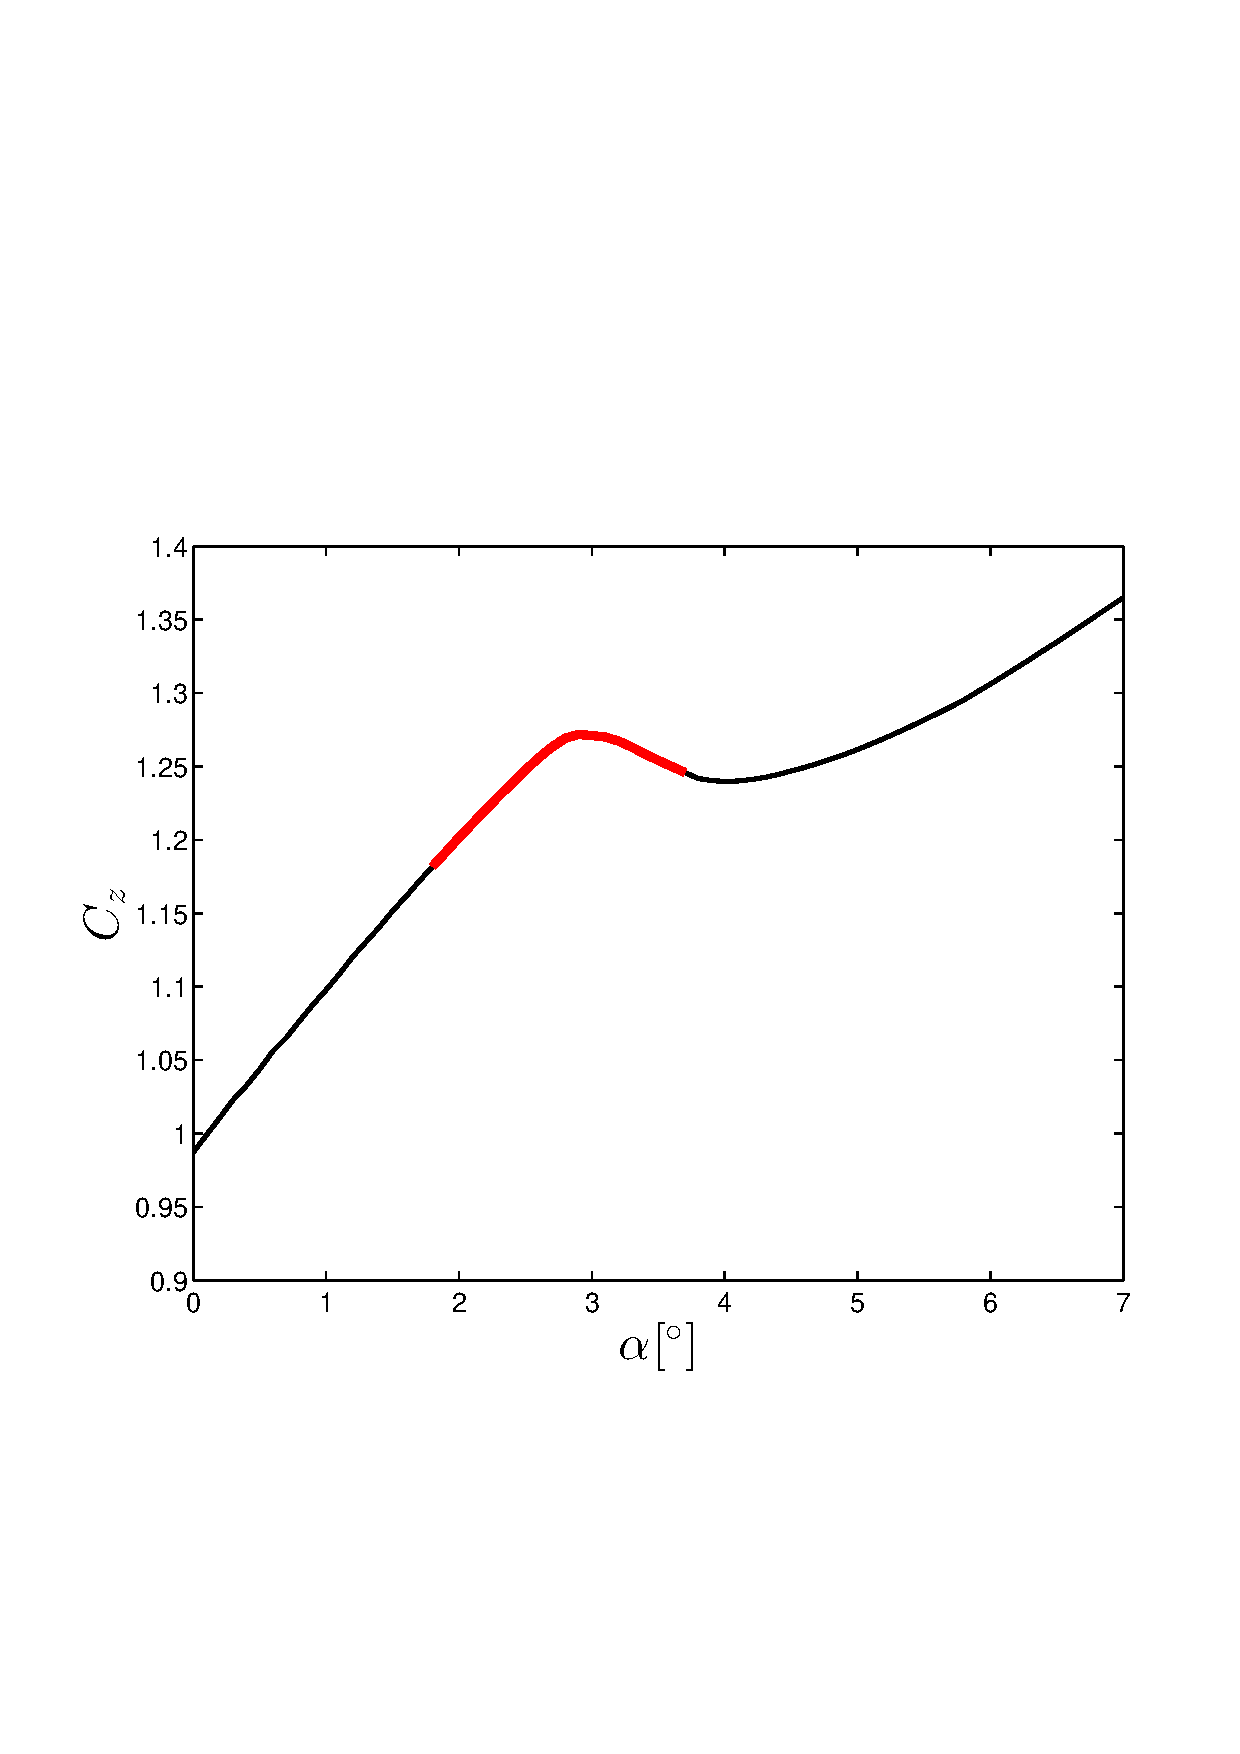
\includegraphics[width=1.0\columnwidth]{nonlinear_cz_re1e6}
		\caption{Static $C_{z}(\alpha)$ curve}
		\label{fig:static_nonlinear}
	\end{subfigure}
	\begin{subfigure}[b]{0.45\textwidth}
		\centering
		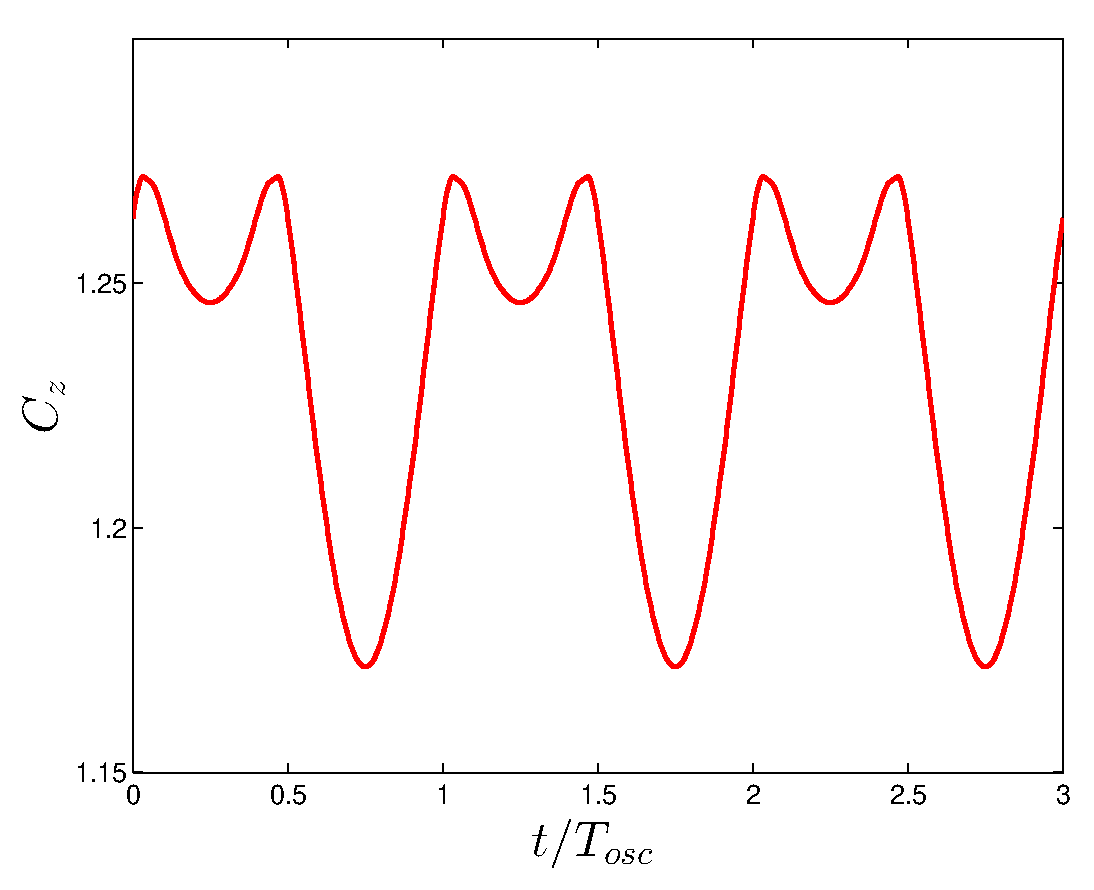
\includegraphics[width=1.0\columnwidth]{dynamic_nonlinear_cz_re1e6}
		\caption{Dynamic response $C_{z}(t)$}
		\label{fig:dynamic_nonlinear}
	\end{subfigure}
	\caption{Quasi-steady response of $C_{z}$ in the non-linear region ($1.7<\alpha<3.7$).}
	\label{fig:nonlinear_cz_response}
\end{figure}
While this may be a hypothetical case, it is reasonable to expect that for a small enough value of $k$, and in the absence of hysteresis there would be no perceptible dynamic effects and the flow would adjust to the slowly varying instantaneous angle of attack. As the value of $k$ is increased and unsteady effects become important, the dynamic response would slowly depart from this quasi-steady response. The simple example suggests that the classical linearized unsteady aerodynamic models, such as the one proposed by \cite{theodorsen35}, are no longer applicable even in the simplest quasi-steady conditions when inherent non-linearities exist in the static case. Unsteady aerodynamic models which account for this non-linearity of the static aerodynamic coefficients are necessary to accurately describe the unsteady response in such conditions.

\section{Stationary airfoil simulations}

\subsection{Parameter identification}

In order to study the dynamic response of unsteady natural laminar flow airfoils, it is necessary to establish the flow conditions for representative static angles of attack. However the high Reynolds numbers of the flow case make it prohibitively expensive to simulate several flow cases at different (static) angles of attack. To reduce the computational cost and narrow down the parameter range, we make use of experimental data provided by \cite{lokattthesis} and also perform calculations using XFOIL. Two factors govern the final choice of parameter selection for the unsteady simulations. 
\begin{itemize}
	\item Firstly, the earlier studies indicate that the dynamic non-linearities are observed when there is a free movement of transition on the suction side of the airfoil \citep{mai11,hebler13,lokattthesis}. Thus the parameter range must have large variations in transition location.  
	\item Secondly, in the previous section we established the link between the non-linearities in the temporal and static responses. Thus we also look for the $\alpha$ range that shows the strongest non-linearities in the static response of the lift coefficient.
\end{itemize}
\begin{figure}[h]
	\centering
	\begin{subfigure}[t]{0.48\textwidth}
		\caption{}		
		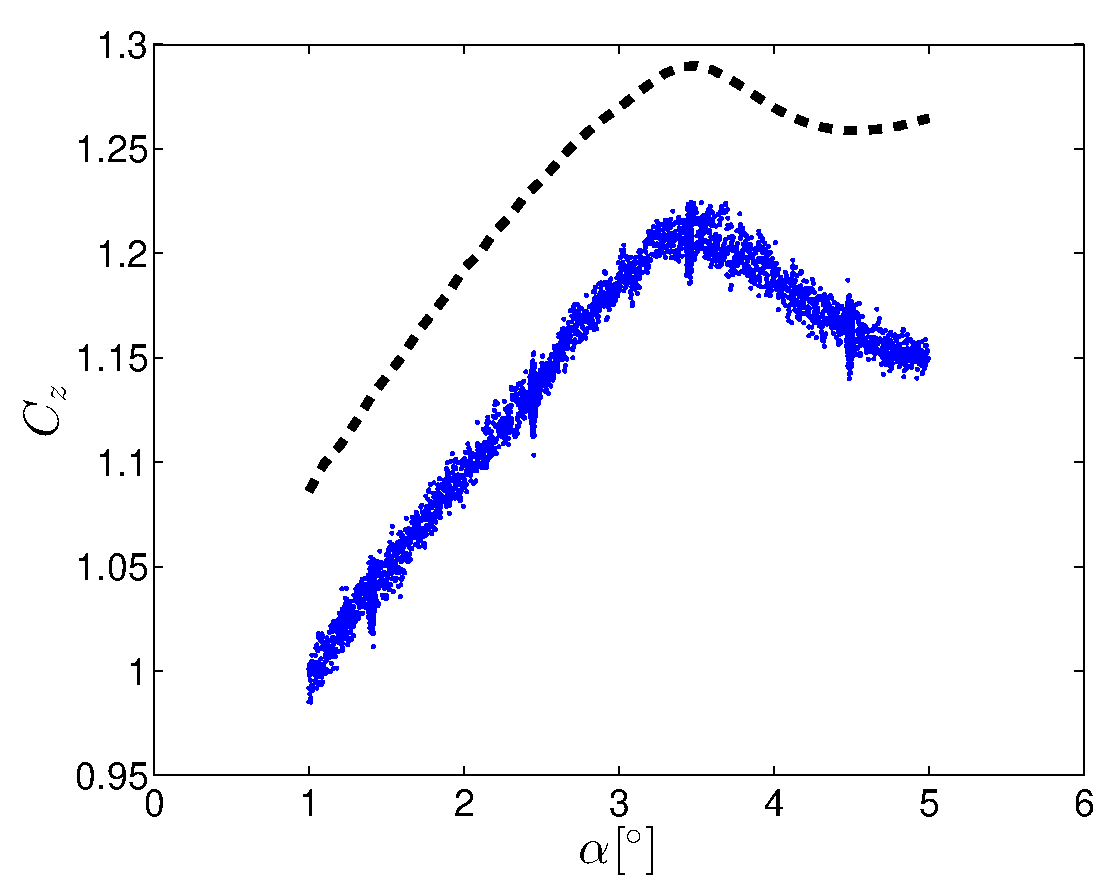
\includegraphics[width=1\textwidth]{765k_static_model_cz_xfoil}
		\label{fig:cz_static_xfoil}
	\end{subfigure}
	\begin{subfigure}[t]{0.48\textwidth}
		\caption{}		
		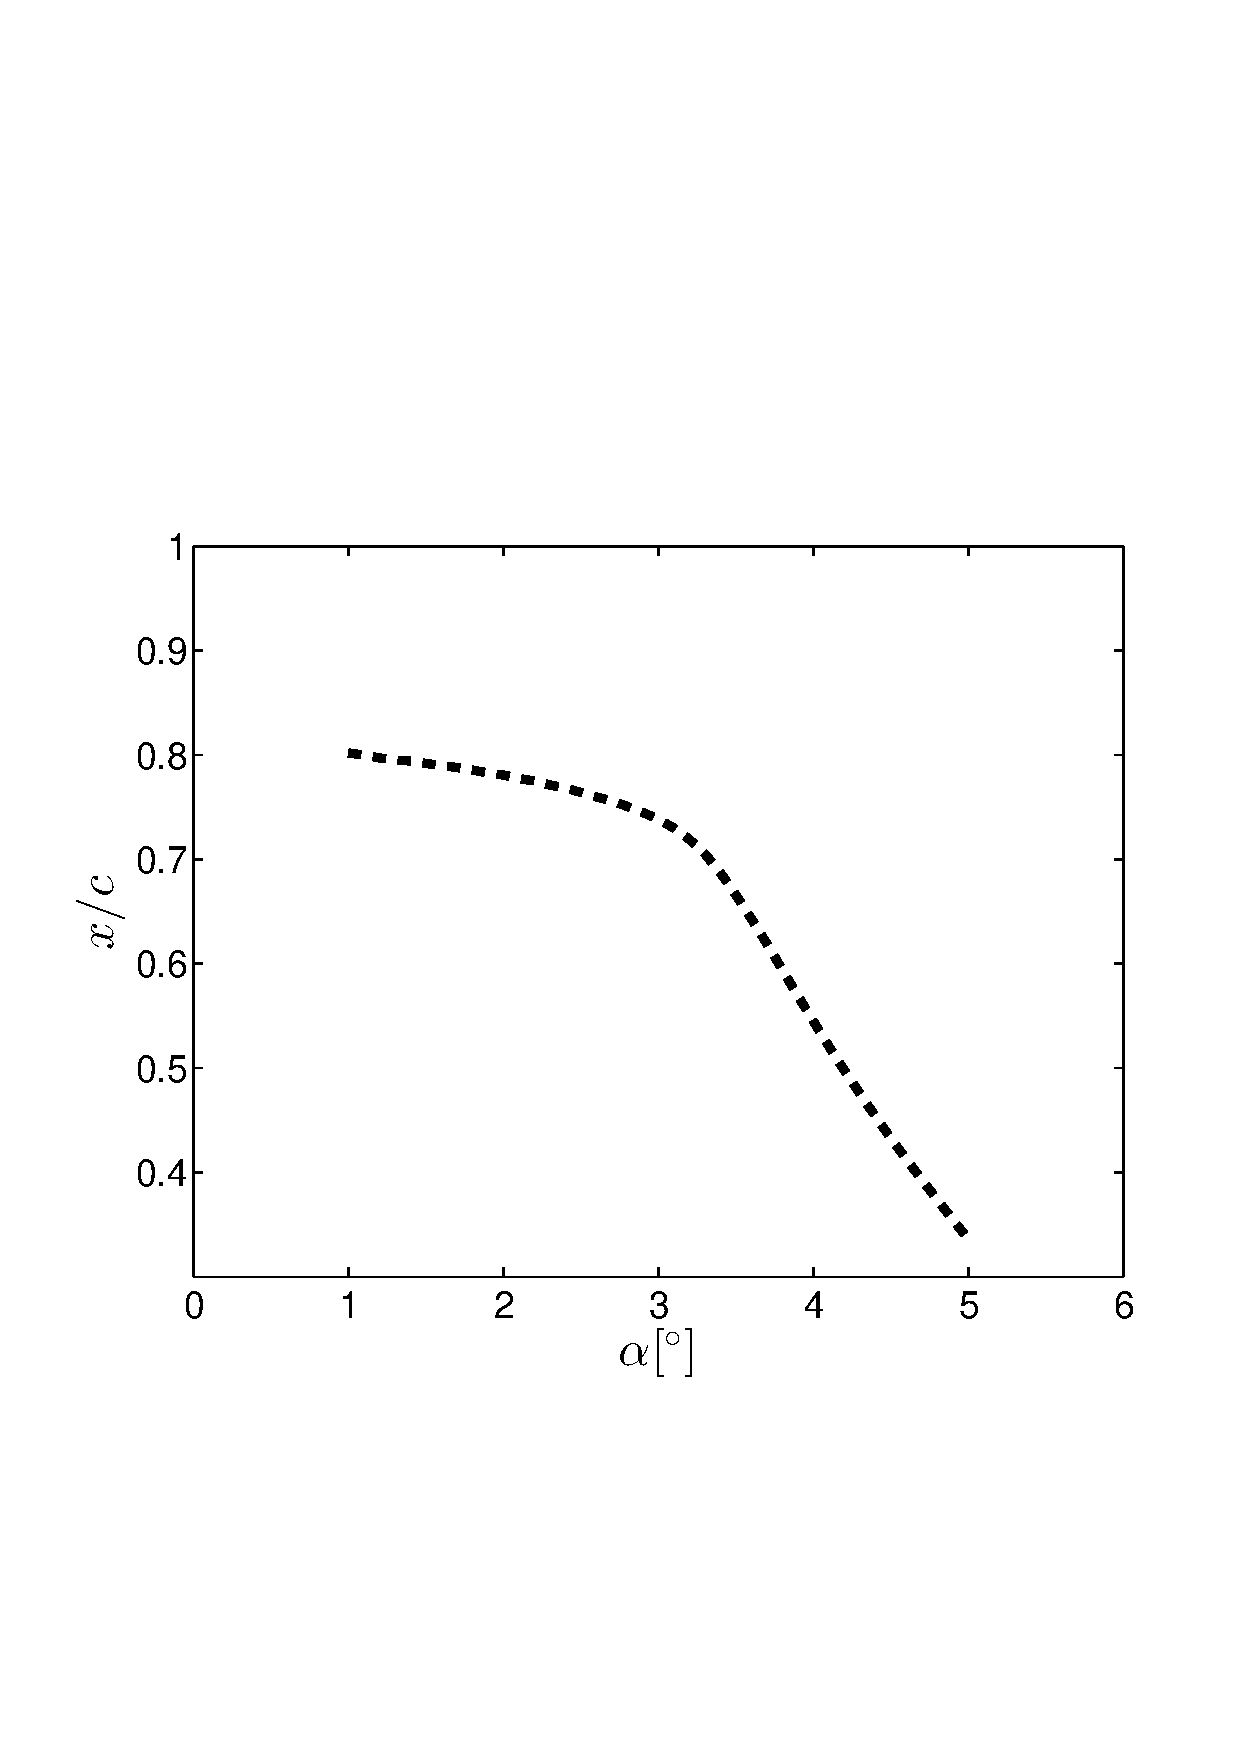
\includegraphics[width=1\textwidth]{765k_static_model_tr_xfoil}
		\label{fig:tr_static_xfoil}
	\end{subfigure}	
	\caption{Static aerodynamic characteristics of the NLF airfoil obtained from XFOIL calculations. Normal force coefficient (left) and transition location (right) variation with $\alpha$.}
	\label{fig:static_characteristics}
\end{figure}
The static response curves for the airfoil obtained using XFOIL as well the experimental data from \cite{lokattthesis} are shown in figure~\ref{fig:cz_static_xfoil}. While the experimental data and XFOIL calculations differ in magnitude, the range of angle of attack where qualitative changes take place is the same. In both cases the static response curve is linear between $1^{\circ}<\alpha<3^{\circ}$ and at around $\alpha=3.4^{\circ}$ the static curves strongly depart from their linear behavior, with the lift coefficient decreasing with increasing $\alpha$. Figure~\ref{fig:tr_static_xfoil} shows the variation of transition location on the suction side of the airfoil as predicted by XFOIL. Within the same range where non-linearities are observed in the static lift coefficient ($\alpha>3.4^{\circ}$), there is a sharp change in the slope of the transition location curve. Between $1^{\circ}<\alpha<3^{\circ}$ the transition location has a very slow upstream movement, while for $\alpha>3.4^{\circ}$, the upstream movement is much more rapid with respect to angle of attack. Both governing factors mentioned earlier indicate the same angle of attack region where non-linearities are to be expected (\textit{i.e} $\alpha\approx3.4^{\circ}$). Thus the pitching range where non-linearities are expected to show up strongly is near $\alpha\approx3.4^{\circ}$. Therefore this is defined as the mean angle of attack of oscillation. The pitch amplitude is taken to be small in accordance with the experimental results of \cite{lokattthesis}. The pitching motion of the unsteady case may be described by equation~\ref{eqn:unsteady_alpha}:
\begin{align}
	\alpha(t) = \alpha_{0} + \Delta\alpha\sin(\Omega (t-t_{0}) + \phi_{0}).
	\label{eqn:unsteady_alpha}
\end{align}
where $\alpha_{0}=3.4^{\circ}$ is the mean angle of attack, $\Delta\alpha=1.0^{\circ}$ is the pitch amplitude, $\Omega$ is the angular frequency of oscillation, $t$ represents the simulation time, $t_{0}$ is the starting time of the pitching motion and $\phi_{0}$ is the initial phase at the start of the oscillations.

In order to verify the static characteristics observed in experiments and also predicted by XFOIL, simulations of stationary airfoils are performed in the range chosen above to ensure that the expected variation of transition location is captured by the numerical simulations. 

\subsection{Computational Setup}

The numerical simulations are set up to perform wall-resolved large-eddy simulations (LESs) of the stationary and pitching airfoils. All numerical simulations are carried out using Nek5000 \citep{nek5000}. The setup is done in a manner very similar to our previous works relating to simulations of flow around airfoils \citep{hosseini16,proc-tsfp10-vinuesa,proc-tsfp10-negi}. The spectral-element mesh is generated using \textit{ANSYS}\textsuperscript{\textregistered} ICEMCFD, which is structured and orthogonal near the airfoil surface. The numerical simulation is set up such that the final resolution utilizes an $11^{th}$ order polynomial representation for the velocity and a staggered $9^{th}$ order representation for the pressure. The Navier--Stokes equations are solved using the Arbitrary-Lagrangian-Eulerian (ALE) framework \citep{ho90,ho91} to account for the motion of boundary and the internal points. The coordinate system is defined such that the $x$ direction is aligned with the inflow direction, $z$ is the spanwise homogeneous direction and $y$ is normal to the airfoil plane. All length scales are normalized by the chord length $c$, and velocities are normalized by the free-stream velocity, $U_{\infty}$. The far field boundaries are two chords away from the airfoil leading edge in either direction and the outflow boundary is four chords downstream from the airfoil leading edge. The inlet is designed as a curved inflow boundary with a constant radial distance of two chords from the leading edge of the airfoil. The spanwise width of the computational domain is $l_{z}=0.15c$. Periodic boundary conditions are imposed on the spanwise boundaries, while the energy-stabilized outflow condition \citep{dong2014} is imposed on the outflow boundary. A URANS simulation is performed using the transition $k$-$\Omega$ SST model \citep{langtry09} for the same case with far-field and outflow boundaries set at a 100 chords distance. Time-averaged velocity field data from the URANS simulation is extracted for the locations corresponding to the domain boundaries of the LES simulation. This extracted data is imposed as a Dirichlet boundary condition on the inlet and far-field boundaries. In order to simulate low turbulence flight conditions, free-stream turbulence of intensity $Ti=0.1\%$ is superimposed on the Dirichlet boundary conditions. The free-stream turbulence is generated using Fourier modes with a von K\'arm\'an spectrum. The integral length scale of the spectrum is set to $l=0.01$ which is approximately 5-10 times the boundary layer height near the leading edge. The procedure is similar to the one described in \cite{schlatterdiploma,brandt04,schlatter08}, where it has been used for the study of by-pass transition in flat-plate boundary layers. It has also been used for wind turbine simulations \citep{kleusberglicenciate} and in our earlier work on pitching airfoils at $Re_{c}=100,000$ \citep{proc-tsfp10-negi}.

The grid resolution on the airfoil surface varies with the chord-wise location in accordance with the changing boundary layer characteristics. Thus the guidelines for grid design use the following criteria:
\begin{itemize}
	\item[$\bullet$] For $0.1<x/c<0.6$, $\Delta x^{+}=18$, $\Delta y_{wall}^{+}=0.64$ and $\Delta y_{max}^{+}=11$, on the suction side and use the local wall-shear ($\tau_{w}$) values on the airfoil. Since the flow is expected to be laminar on the pressure side, the stream-wise resolution is slightly relaxed to $\Delta x^{+}=25$ while keeping the same wall-normal resolution.
	\item[$\bullet$] For $x/c<0.1$, the peak $\tau_{w}$ value over the suction side of the airfoil is used to estimate the grid spacing for both the suction and pressure sides.
	\item [$\bullet$] for $x/c>0.6$, the suction side experiences a large adverse pressure gradient which significantly reduces $\tau_{w}$ values. Therefore, the $\tau_{w}$ values from the pressure side are used for both the suction and pressure sides.
	\item [$\bullet$] A structured mesh is used, which is extruded in the span-wise direction. Hence the spanwise resolution is constant throughout the domain. The resolution is set to $\Delta z^{+}=12$, where the the peak $\tau_{w}$ value from the suction side is used.
\end{itemize}
The symbol $^{+}$ indicates normalization with inner units using kinematic viscosity $\nu$, and local friction velocity $u^{*}$. Wall-shear stress data is obtained using XFOIL to estimate the local friction velocity. A trip is introduced in XFOIL at $x/c\approx0.1$ to obtain turbulent wall-shear values on both the suction and pressure sides of the airfoil. A different criterion is needed for defining the resolution in the wake where the wall-based criteria are not valid. Accordingly, the URANS data is used to estimate the Kolmogorov length scale ($\eta$) in the wake region. The grid in the wake region is designed such that the average grid spacing in the near wake ($1<x/c<2$) follows the criteria: $\Delta x/\eta < 9$. For $x/c>2$ the grid spacing in the wake is slowly increased such that $\Delta x/\eta \approx 20$ near the outflow boundary at $x/c=4$.

Note that the above guidelines are for the final resolution of the numerical simulation. In our methodology we simulate the initial transients with a lower order polynomial representation on the same spectral-element grid and slowly increase the polynomial order. Currently, only the results from the low order polynomial simulations ($5^{th}$ order for the velocity) are reported. The effective grid spacings for the current results is therefore twice the values reported above. Nonetheless, tests with stationary airfoil simulations indicate that the qualitative features of the flow do not change with changing polynomial orders. 

\subsection{Stationary simulation results}

In accordance with the angle of attack range selected earlier, we perform two simulations with a stationary airfoil, with angles of attack corresponding to the two extremities of the pitching cycle, \textit{i.e.} at $\alpha=2.4^{\circ}$ and $\alpha=4.4^{\circ}$. Figure~\ref{fig:la2_750k_stationary} shows the instantaneous vortical structures identified by the $\lambda_{2}$ criterion \citep{jeong95}. From the figures it is clear that the transition occurs at widely different chord-wise locations for the two angles of attack, which is in accordance with the predictions of XFOIL as seen earlier in figure~\ref{fig:tr_static_xfoil}.
\begin{figure}[h]
	\centering
	\begin{subfigure}[t]{0.9\textwidth}
		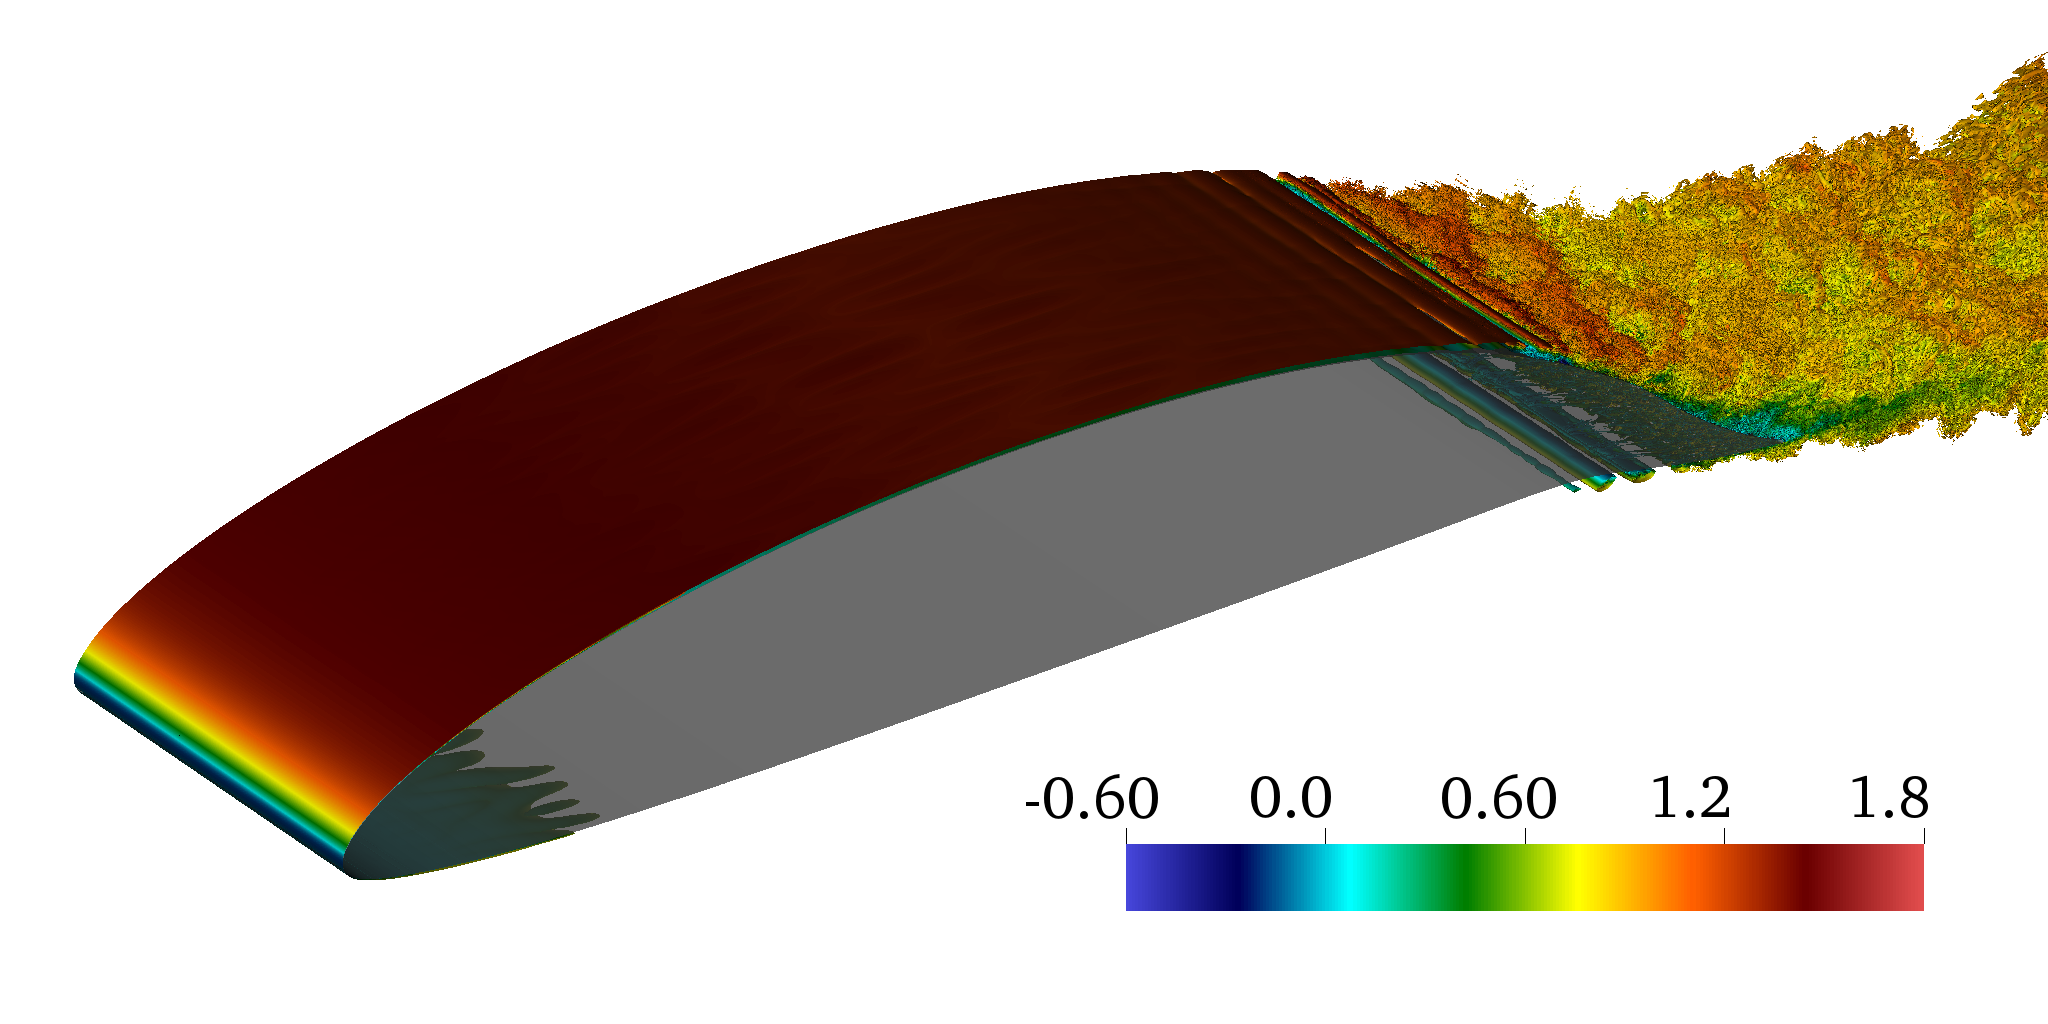
\includegraphics[width=1\textwidth]{pitch_re750k0001}
		\caption{$\alpha=2.4^{\circ}$}
		\label{fig:la2_aoa24}
	\end{subfigure}
	\begin{subfigure}[t]{0.9\textwidth}
		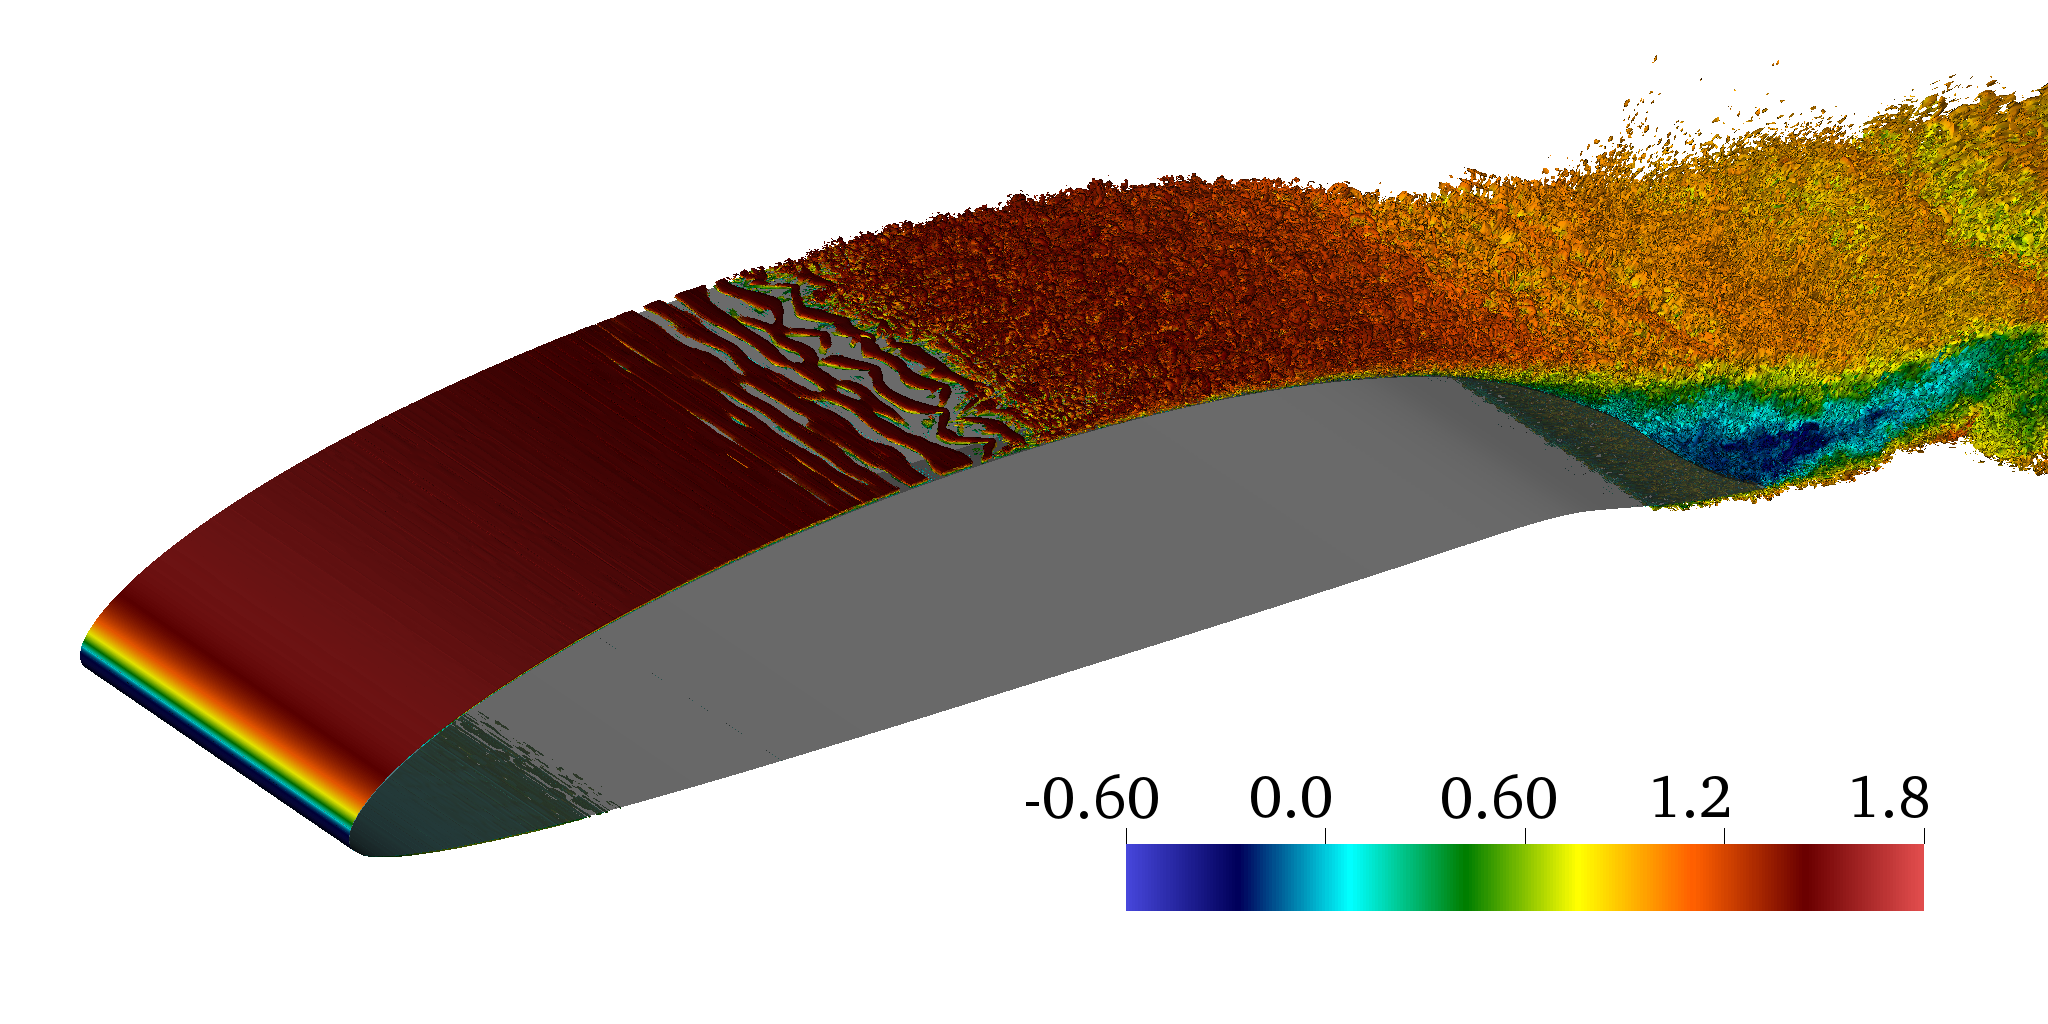
\includegraphics[width=1\textwidth]{pitch_re750k0002}
		\caption{$\alpha=4.4^{\circ}$}
		\label{fig:la2_aoa44}		
	\end{subfigure}	
	\caption{Instantaneous vortical structures identified by the $\lambda_{2}$ criterion for the two stationary angle of attack simulations.}
	\label{fig:la2_750k_stationary}
\end{figure}
The instantaneous structures for both cases are extracted after running the two simulations for about 6 flow through times. After the initial transients are convected away, the overall qualitative state of the flow does not change and the transition location remains constant. To ensure that the low order of the simulations is not affecting the transition location, and thus the overall qualitative flow state, the simulation with the lower angle of attack ($\alpha=2.4^{\circ}$) is restarted with a higher polynomial order ($N=8$) and the simulation is continued for about 1 flow over time. No qualitative change is detected in the flow state and the transition location does not change.

\section{Unsteady results}

\subsection{Lift coefficient}
Once the flow state for the stationary airfoil cases is established, oscillations of a pitching airfoil are performed with the pitching motion prescribed by equation~\ref{eqn:alpha_inst}. The angular frequency ($\Omega$) of the oscillation is chosen such that the non-dimensional reduced frequency, $k=0.4$ and the pitch axis is located at $(x_{0},y_{0})=(0.35,0.034)$. The time period of oscillation ($T_{osc}$) for the chosen reduced frequency is equal to $7.85$. The pitching simulations are started from the solutions of the stationary airfoil simulation at the angle of attack of $\alpha=2.4^{\circ}$. This point represents the minimum of the pitch cycle and starting the pitching motion from this minimum allows us to smoothly increase the angular velocity from zero. Thus no impulsive velocities are imparted to the airfoil when the pitching motion starts. The oscillatory motion is thus prescribed by equation~\ref{eqn:unsteady_alpha_2}:
\begin{subequations}
	\begin{align}
		\alpha(t) = \alpha_{0} + \Delta\alpha\sin(\Omega (t-t_{0}) + \phi_{0}), %\\
	%	\alpha_{0}=3.4^{\circ} & \Delta\alpha=1.0^{\circ} & t_{0}=6.0 & \beta=-\pi/2 \nonumber	
	\end{align}
	\begin{align}
		\text{with}\hspace{10pt}\alpha_{0}=3.4^{\circ}, \hspace{20pt} & \Delta\alpha=1.0^{\circ}, & t_{0}=6.0\hspace{10pt} \text{and} \hspace{10pt}& \phi_{0}=-\pi/2.
	%\label{eqn:unsteady_alpha_parameters}	
	\end{align}
\label{eqn:unsteady_alpha_2}
\end{subequations}
\begin{figure}[h]
	\centering
	\begin{subfigure}[t]{0.48\textwidth}
		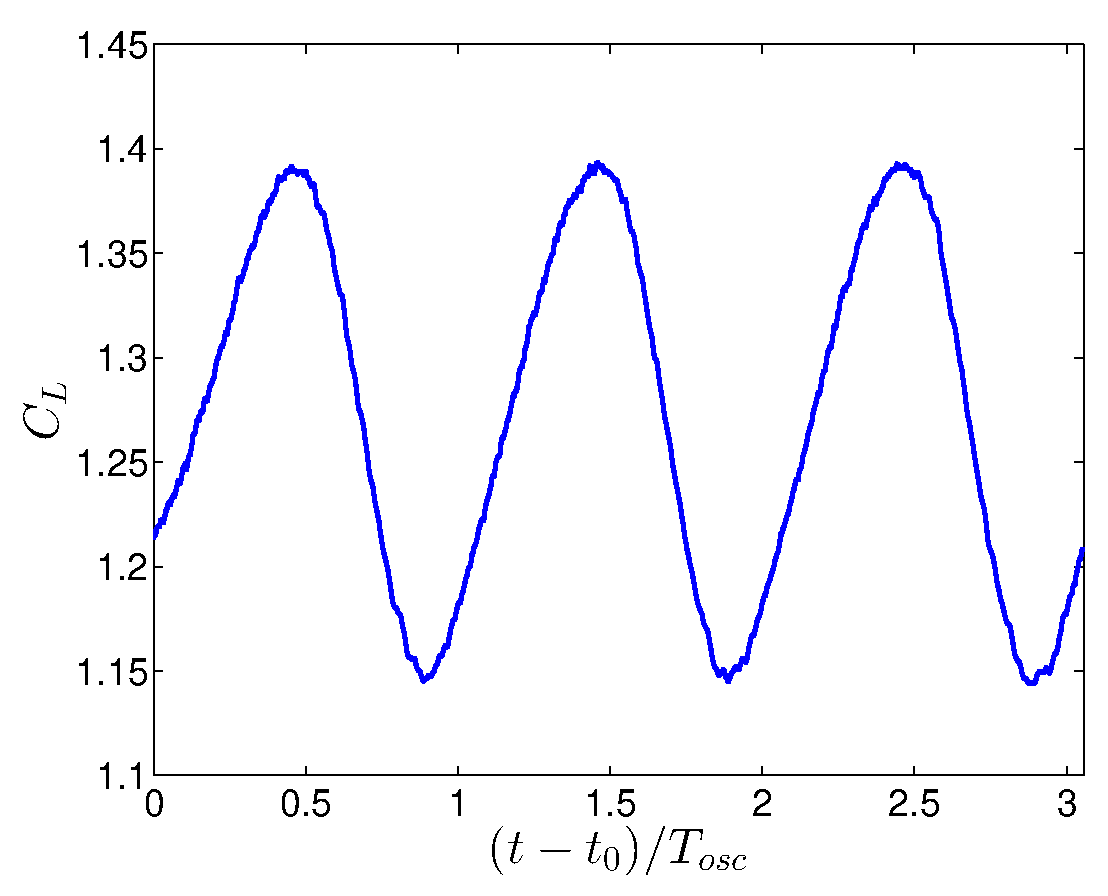
\includegraphics[width=1\textwidth]{cl-time-alpha750k}
		\caption{}
		\label{fig:750k_cl_time_alpha}		
	\end{subfigure}
	\begin{subfigure}[t]{0.495\textwidth}
		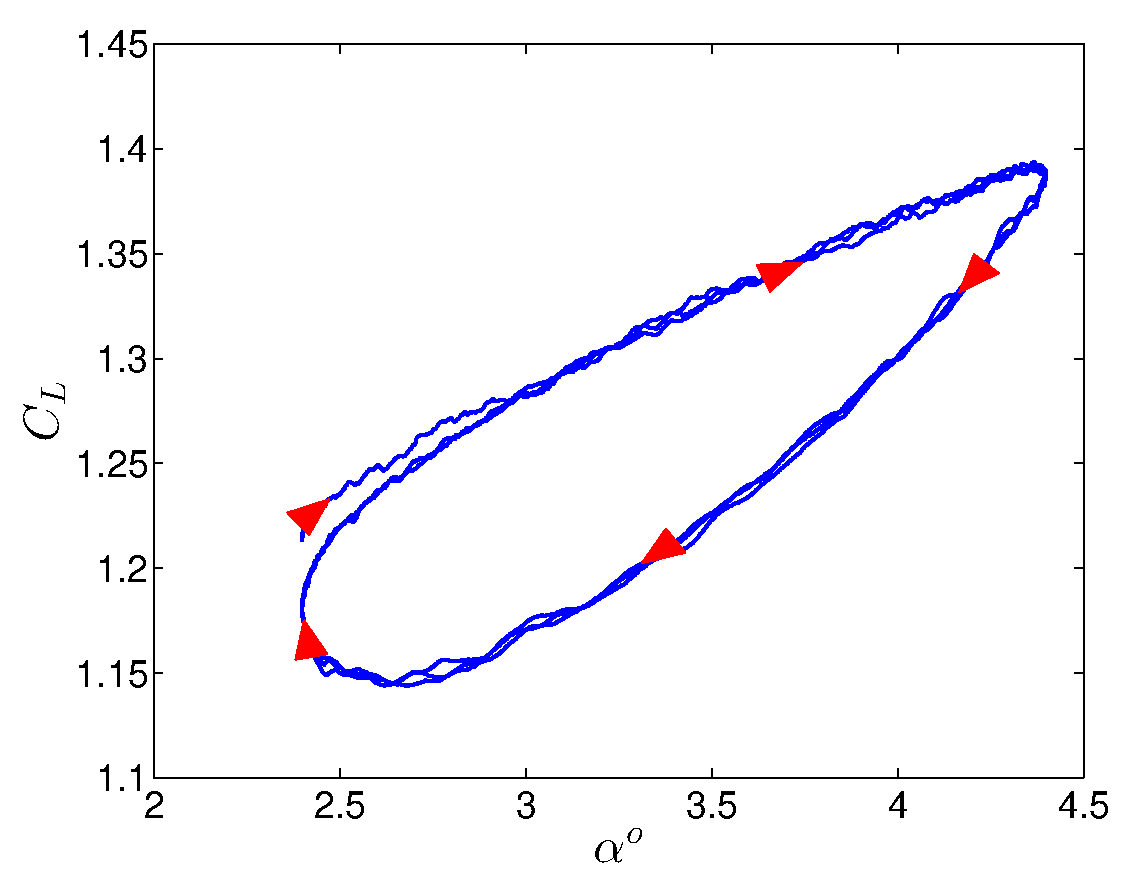
\includegraphics[width=1\textwidth]{cl-alpha750k}
		\caption{}
		\label{fig:750k_cl_alpha}			
	\end{subfigure}	
	\caption{Variation of unsteady lift coefficient with time (left) and instantaneous angle of attack (right). Red arrows in the phase portrait indicate direction of time.}
	\label{fig:750k_unsteady_lift}
\end{figure}

Figure~\ref{fig:750k_unsteady_lift} shows the variation of the unsteady lift coefficient $C_{L}$ with time, as well as the phase portrait with respect to $\alpha$. One can immediately observe from the phase portrait (figure~\ref{fig:750k_cl_alpha}) that (after a small initial transient) no large deviations of the lift coefficient occur between consecutive cycles of oscillation, indicating that the flow has settled into a regular cyclic state and further qualitative changes that may be transient in nature are not expected to occur with more pitch cycles. While the non-linearity is less obvious from the time series plot, the phase portrait clearly shows the non-linearities by way of a distorted ellipse. Linear responses trace an ellipse in the phase portrait with respect to angle of attack. Distortions of the ellipse indicate the presence of additional frequencies in the time response.

\subsection{Unsteady boundary layer}
The spatio-temporal variation of the boundary layer can be analyzed via the instantaneous wall-shear stress. Figure~\ref{fig:space-time_color750k} shows the space-time variation of the instantaneous, spanwise averaged wall-shear stress on the suction side of the airfoil surface. Areas which are strongly red in color are high shear-stress regions and thus signify turbulent flow (except the region very close to the leading edge which has a very thin boundary layer). The turbulent regions show periodic bumps in the space-time plot which are indicative of the movement of transition throughout the oscillation phases. This is consistent with the earlier studies of \cite{mai11,hebler13} and \cite{lokattthesis} which suggest the free movement of transition is responsible for non-linearities in the aerodynamic force coefficients. Figure~\ref{fig:750k_cf_x} shows horizontal slices from the space-time plot for two different time instants which represent the instantaneous spatial variations of $\tau_{w}$.  
\begin{figure}[!h]
   	\centering
	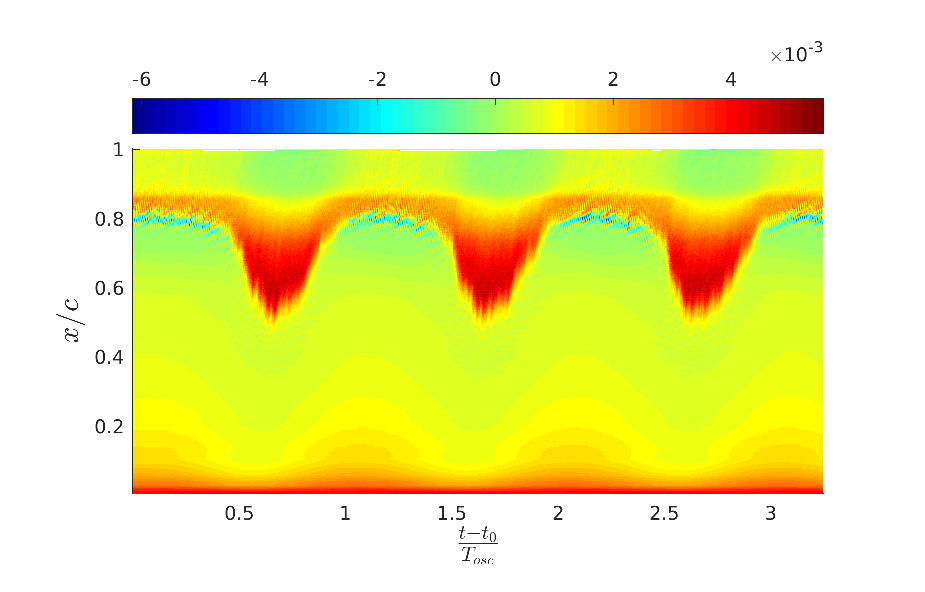
\includegraphics[width=\textwidth]{cf_time_surf750k}		
	\caption{Spatio-temporal variation of wall-shear stress. The $y$-axis represents the chord-wise location while the $x$-axis represents the normalized simulation time. The colors represent the instantaneous, spanwise-averaged wall-shear stress value, $\tau_{w}(x,t)$, for each chord-wise location.}	
	\label{fig:space-time_color750k}
\end{figure}
\begin{figure}[!h]
	\centering
	\begin{subfigure}[t]{0.49\linewidth}
		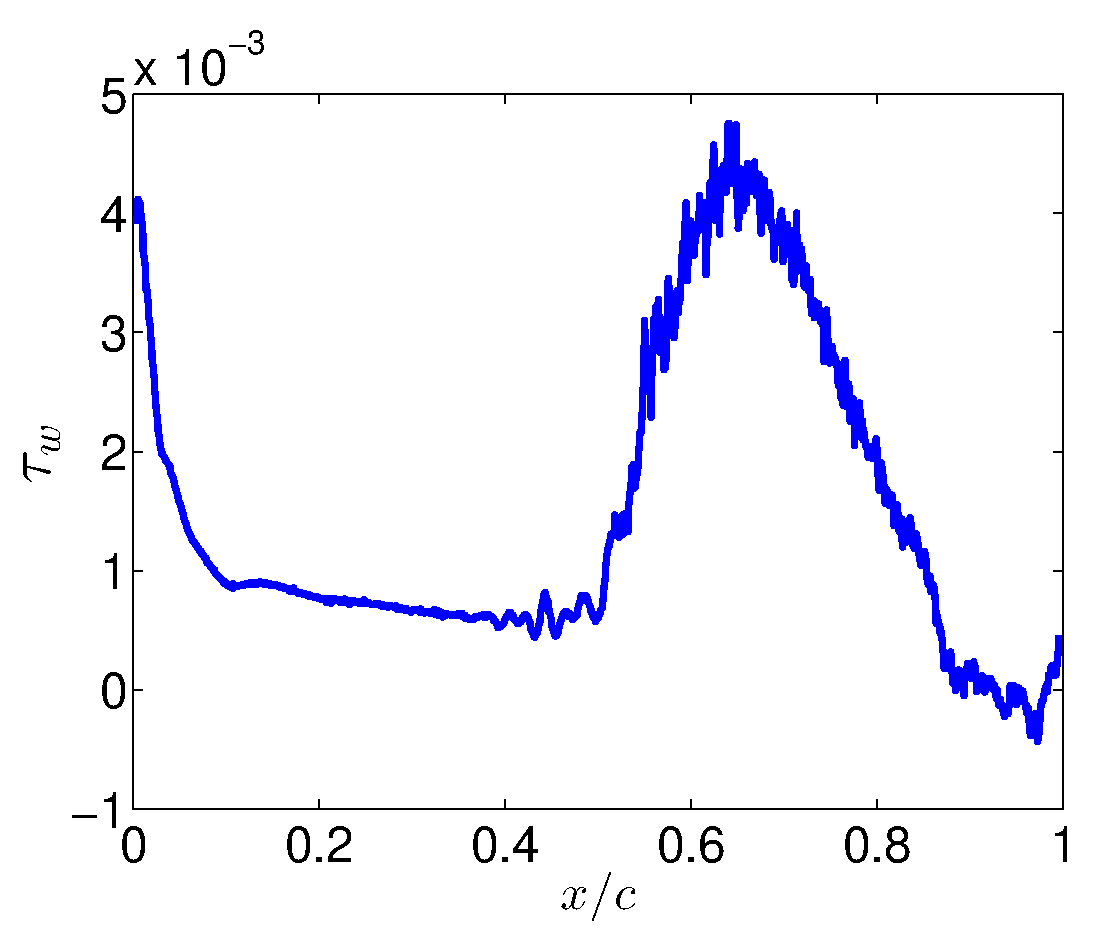
\includegraphics[width=\linewidth]{pitch750k_t01_60}
%		\label{fig:750k_cf_x_t1.60}
	\end{subfigure}
	\begin{subfigure}[t]{0.49\textwidth}			
		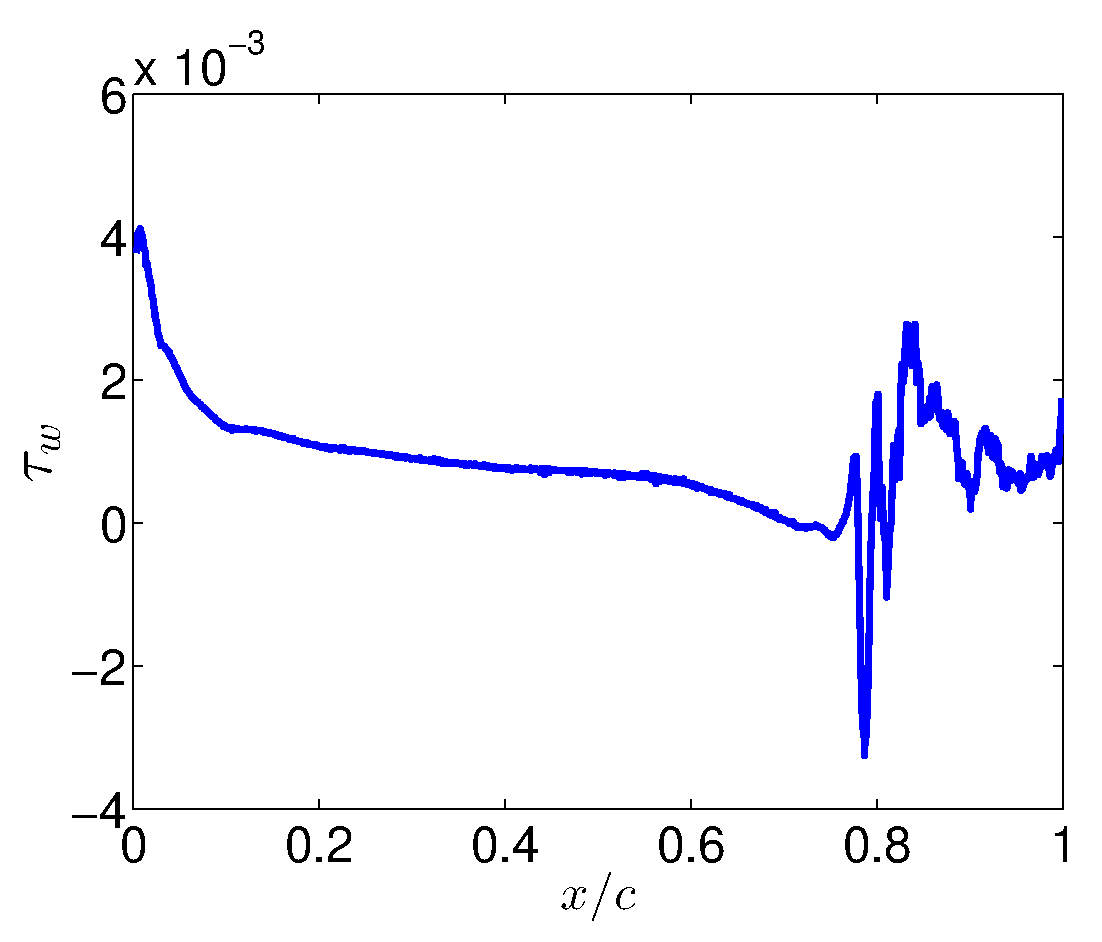
\includegraphics[width=\linewidth]{pitch750k_t02_25}
%		\label{fig:750k_cf_x_t2.25}
	\end{subfigure}
	\caption{Instantaneous chord-wise variation of $\tau_{w}(x,t)$. Figures represent time-instants when the transition is close to its most upstream location at time $(t-t_{0})/T_{osc}=1.60$ (left) and when it is close to the most downstream location at time $(t-t_{0})/T_{osc}=2.25$ (right).}
	\label{fig:750k_cf_x}	
\end{figure}

%\begin{figure}[h]
%   	\centering
%   	\begin{minipage}{0.55\linewidth}
%   		\begin{subfigure}[t]{\linewidth}
%   			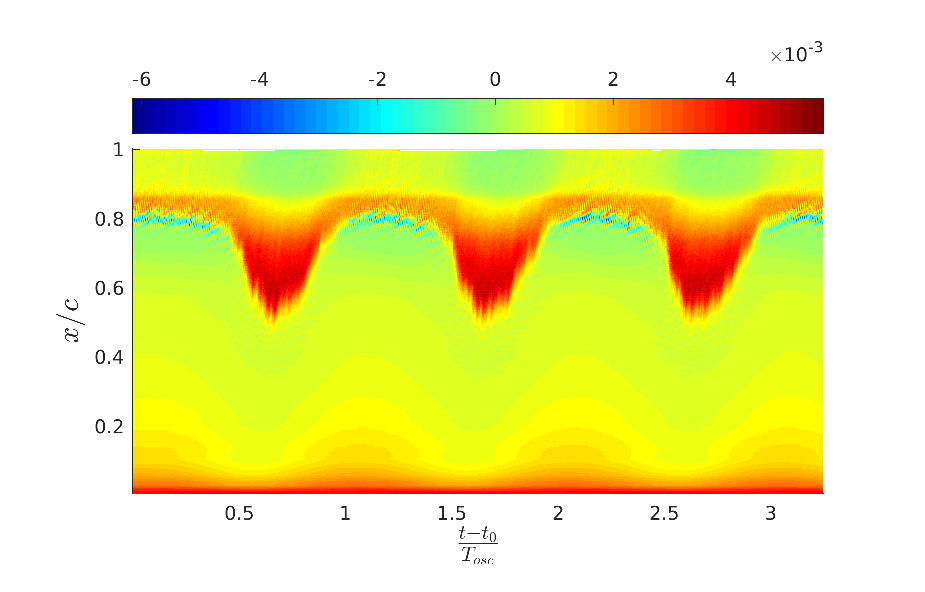
\includegraphics[width=\linewidth]{cf_time_surf750k}
%   			\caption{Spatio-temporal evolution of $\tau_{w}$}
%   			\label{fig:space-time_color750k}
%   		\end{subfigure}
%   	\end{minipage}   	
%   	\begin{minipage}{0.44\linewidth}
%   		\begin{subfigure}[t]{\linewidth}
%   			\caption{}   			
%   			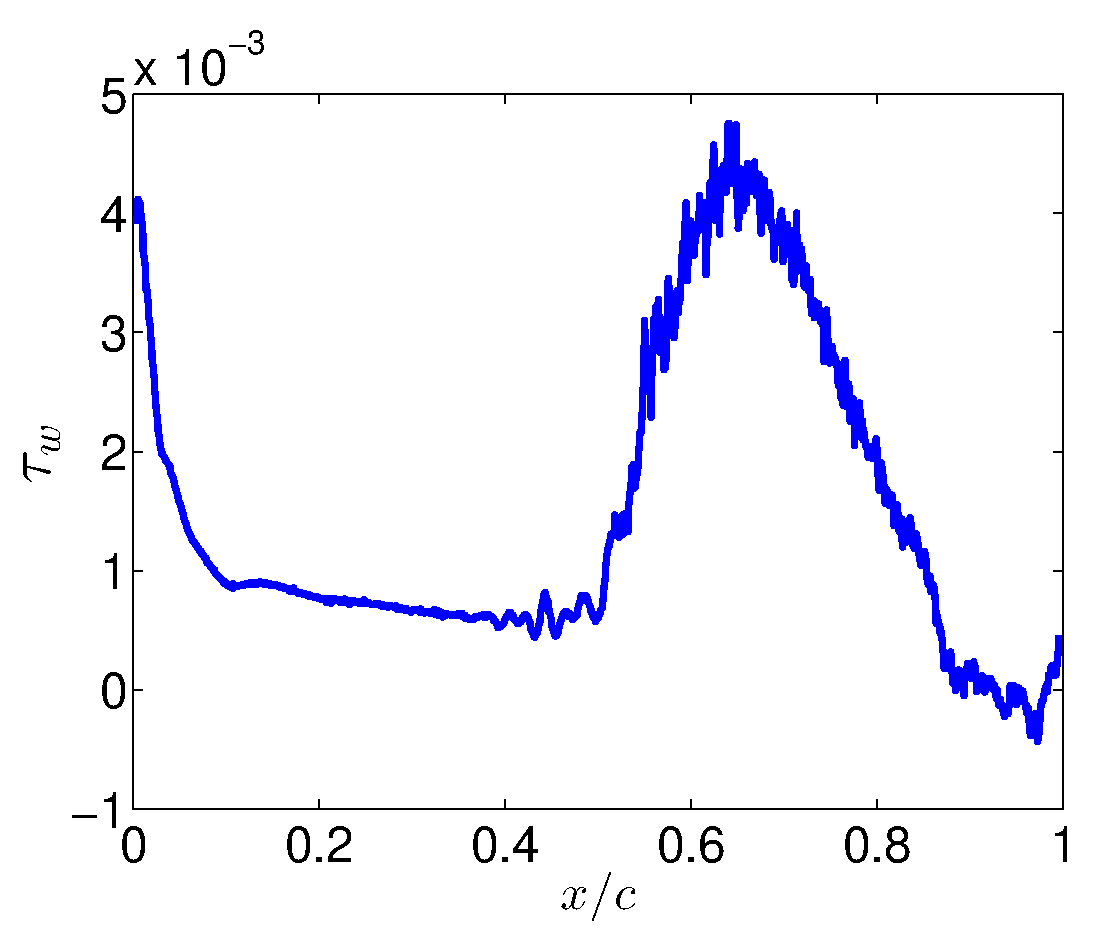
\includegraphics[width=\linewidth]{pitch750k_t01_60}
%   			\label{fig:750k_cf_x_t1.60}
%   		\end{subfigure}
%   		\begin{subfigure}[t]{\textwidth}
%   			\caption{}   			
%   			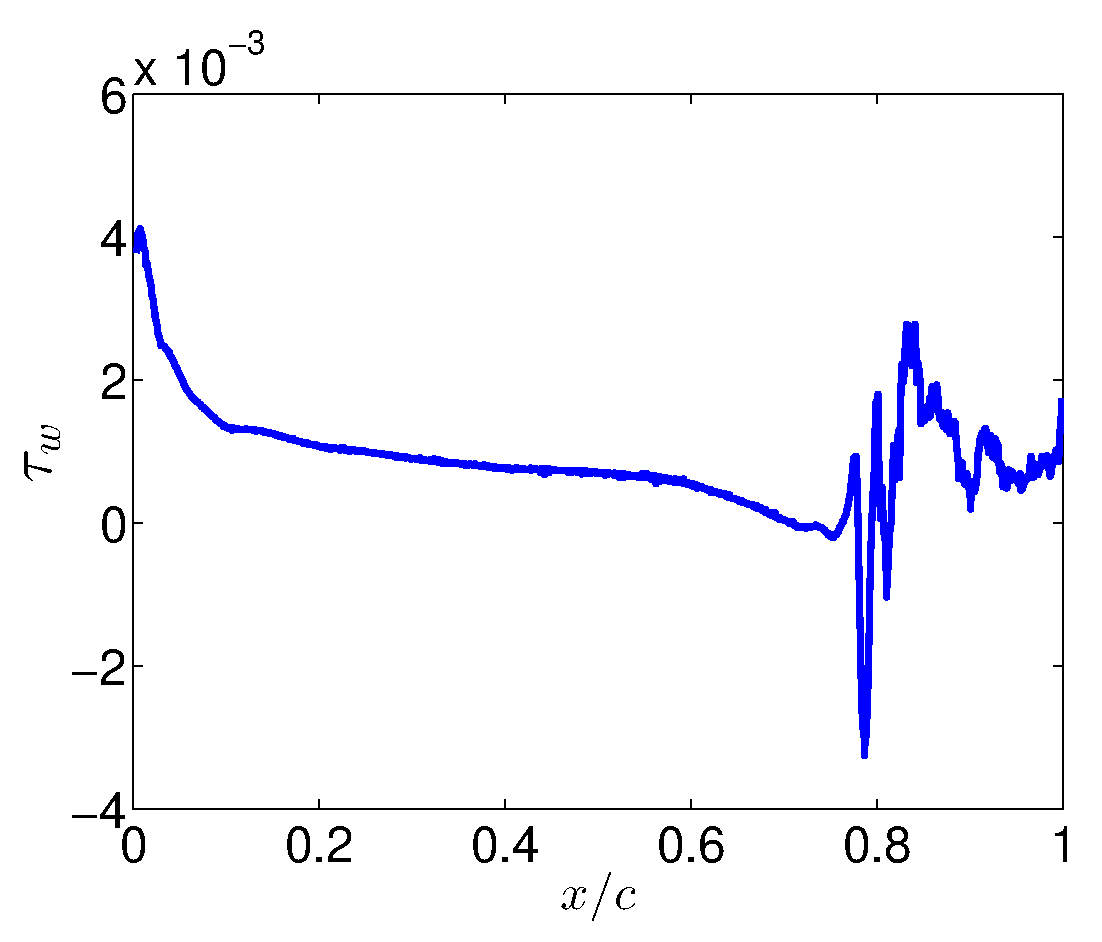
\includegraphics[width=\linewidth]{pitch750k_t02_25}
%   			\label{fig:750k_cf_x_t2.25}
%   		\end{subfigure}
%   	\end{minipage}
%   	\hfil
%   	\caption{The color plot on the left (a) shows the space-time variation of wall-shear stress. The $x$-axis represents the chord-wise location while the $y$-axis represents the normalized simulation time. The colors represent the instantaneous, spanwise averaged wall-shear stress value, $\tau_{w}(x,t)$, for each chord-wise location. Figures on the right show the chord-wise variation of $\tau_{w}(x,t)$ at two different time instances when the transition is close to its most upstream location at time $(t-t_{0})/T_{osc}=1.60$ (b) and when it is close to the most downstream location at time $(t-t_{0})/T_{osc}=2.25$ (c).}
%   	\label{fig:space-time_cf750k}
%\end{figure}

\subsection{Transition location}
For further analysis a quantification of the transition point variation is necessary and to this end the instantaneous transition point needs to be defined. Since the transition changes continuously with time, a criterion is required which is based on the instantaneous state of the flow rather than the long-time statistical average. In order to define quantities representative of the instantaneous state of the flow, we take advantage of the homogeneous direction and and also perform a temporal averaging operation for a very short duration in time. Thus we evaluate statistical quantities ``$\overline{q}(x,y,t)$'' which are defined as in equation~\ref{eqn:750k_inst_q}:
\begin{align}
	\overline{q}(x,y,t) = \left(\frac{1}{z_{max}-z_{min}}\right)\left(\frac{1}{\Delta t}\right)\int_{t'=t}^{t'=t+\Delta t}\int_{z=z_{min}}^{z=z_{max}}q(x,y,z,t')\ dz\ dt'.
	\label{eqn:750k_inst_q}
\end{align}
Here $(z_{max} - z_{min})$ is the spanwise width of the computational domain and $\Delta t$ is a short temporal averaging period. In order for such a quantity to be representative of the instantaneous state of the flow, the time duration of the averaging must be small. For the current case we use $\Delta t=3\times10^{-2}$, which amounts to $0.38\%$ of the oscillation time period during which the flow can be assumed to remain approximately in the same state. Using this procedure we evaluate the fluctuating Reynolds stress, $\overline{u'v'}(x,y,t)$. Large Reynolds stresses indicate turbulent flow, thus the most upstream location (on the suction side) where the the quantity $\overline{u'v'}(x,y,t)$ becomes large is denoted as the transition location. In order to prescribe a suitable threshold for ``large", the maximum value of $|\overline{u'v'}(x,y,t)|$ across the entire boundary layer is evaluated for all times. This maximum value does not have very large variations, staying within the same order of magnitude with its mean value being $|\overline{u'v'}|_{max}=10^{-2}$. The threshold for determining transition is set to $5\%$ of this value. The transition point is thus the first point where $|\overline{u'v'}(x,y,t)|>5\times10^{-4}$. Since the criterion is a bit arbitrary, it is cross-checked by evaluating the variance of the spanwise velocity fluctuations $\overline{w'w'}(x,y,t)$ following the same procedure. In this case the threshold is set as $|\overline{w'w'}(x,y,t)|>10^{-3}$, since the peak spanwise fluctuation intensity is found to be nearly twice the peak Reynolds stress. Growing spanwise velocity fluctuations indicate the onset of three-dimensionality, and thus they constitute a physically meaningful indicator of transition. Despite the rather ad-hoc nature of the threshold criteria, the qualitative picture of transition movement is not very sensitive to small changes in the threshold. Reducing or increasing the thresholds by a factor of 2 still produces the same qualitative trends (not shown). Figure~\ref{fig:750k_tr_alpha} shows the phase portrait of the transition location, determined by the aforementioned criteria. The two criteria show a good quantitative agreement with each other. Figure~\ref{fig:750k_space-time_tr} shows the calculated transition location (using $\overline{u'v'}$) superposed on the wall-shear stress space-time plot. The calculated transition locations are consistent with the picture of wall-shear stress with transition marginally preceding regions of turbulent flow.

%\begin{figure}[43]{r}{0.58\textwidth}
%	\centering	
%	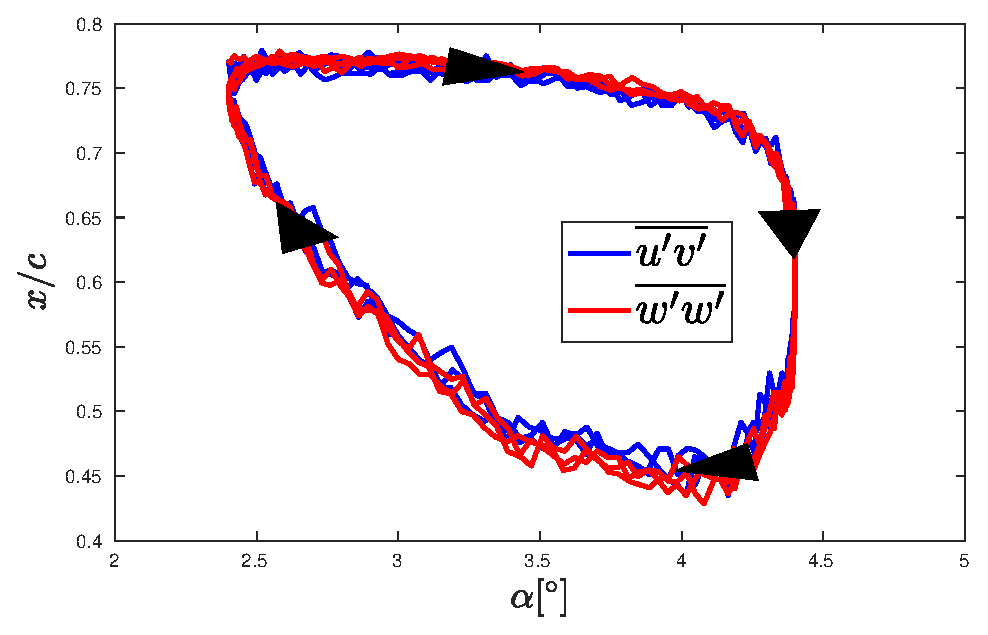
\includegraphics[width=0.50\textwidth]{750k_transition_alpha}
%	\caption{Empirically determined transition location using the $|\overline{u'v'}|$ and $|\overline{w'w'}|$ criteria. Arrows indicate the forward direction in time.}
%	\label{fig:750k_tr_alpha}
%	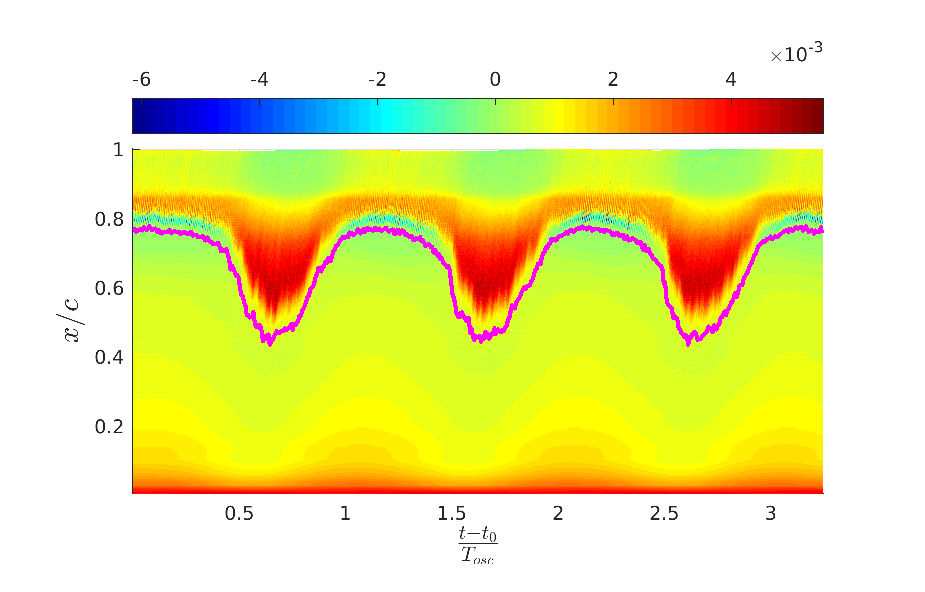
\includegraphics[width=0.55\textwidth]{cf_time_surf750k_tr}
%	\caption{Empirically determined transition location (magenta curve) overlay-ed on the space-time plot of $\tau_{w}$.}
%	\label{fig:750k_space-time_tr}
%\end{figure}

\begin{figure}[h]
	\centering	
	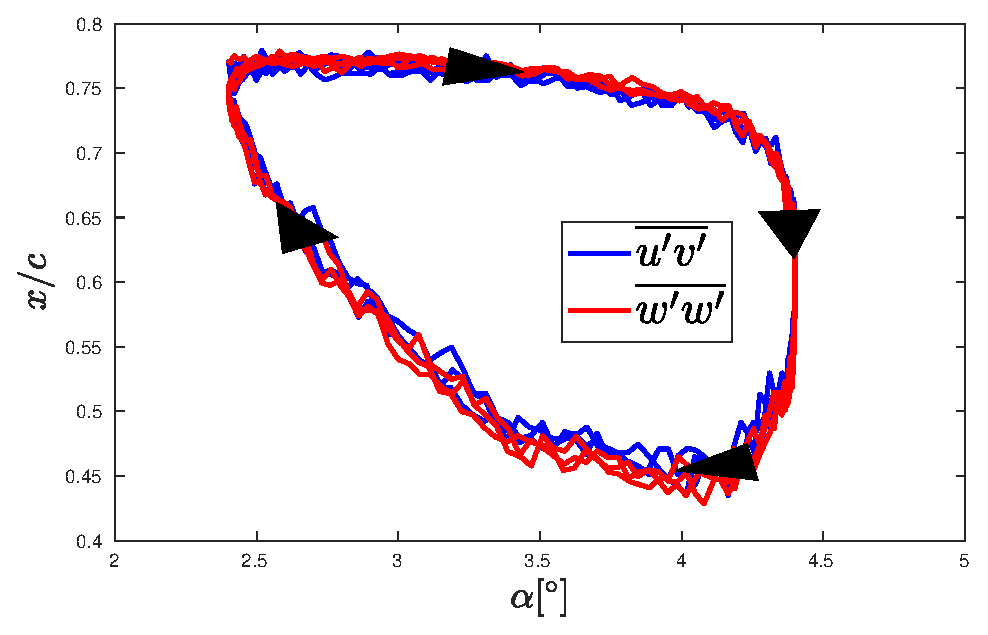
\includegraphics[width=0.60\textwidth]{750k_transition_alpha}
	\caption{Empirically determined transition location using the $|\overline{u'v'}|$ and $|\overline{w'w'}|$ criteria. Arrows indicate the forward direction in time.}
	\label{fig:750k_tr_alpha}
\end{figure}
\begin{figure}
	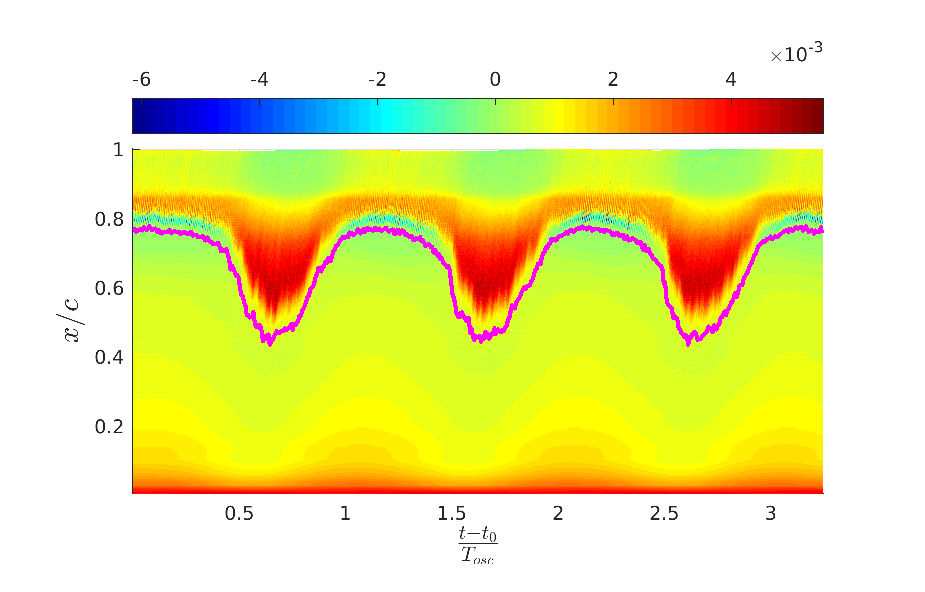
\includegraphics[width=\textwidth]{cf_time_surf750k_tr}
	\caption{Empirically determined transition location (magenta curve) superposed on the space-time plot of $\tau_{w}$.}
	\label{fig:750k_space-time_tr}
\end{figure}

The phase portrait in figure~\ref{fig:750k_tr_alpha} clearly shows the asymmetric flow states between the pitch-up (upper branch) and the pitch-down (lower branch) phases of the oscillation. During the pitch-up phase the transition point is near the trailing edge and has a very slow upstream movement for most part of pitch-up cycle, and later moves upstream sharply at the end of the pitch-up phase. During the pitch-down phase of the oscillation, the transition location is constantly moving downstream with the motion appearing much more gradual in phase space. This phase portrait can be transformed to give a more insightful picture of the ongoing dynamics by using a phase-lag concept. In this transformation we consider the evolution of the boundary layer with respect to an effective angle of attack $\alpha_{e}$ which differs from the instantaneous angle of attack by a phase-lag. The physical interpretation of the phase-lag is a simple one, \textit{i.e.} the boundary layer adjusts to the changing flow-field in a quasi-steady manner, however there is a time lag between the airfoil motion and the boundary-layer adjustment, and the effective angle of attack that the boundary layer perceives is different from the instantaneous angle of attack. The expression for the effective angle of attack for the current case may be written by adding an additional term to equation~\ref{eqn:unsteady_alpha_2}
\begin{align}
	\alpha_{e}(t) = \alpha_{0} + \Delta\alpha\sin(\Omega (t-t_{0}) + \phi_{0} + \boldsymbol{\phi_{lag}}),
	\label{eqn:unsteady_alpha_3}
\end{align}
where $\boldsymbol{\phi_{lag}}$ is the phase lag between the instantaneous and effective angles of attack.
%\begin{wrapfigure}[22]{R}{0.58\textwidth}
%	\centering
%	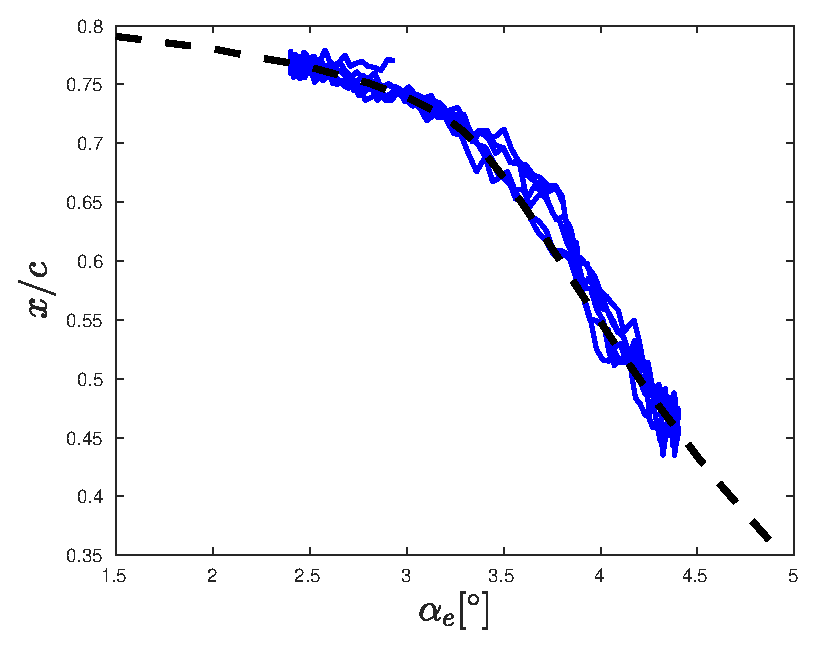
\includegraphics[width=0.56\textwidth]{750k_transition_alpha_e}
%	\caption{Phase portrait of the transition location with respect the effective angle of attack($\alpha_{e}$). The blue lines represent the evaluated transition location (using $|\overline{u'v'}|$) and the black dashed line represents static transition location values obtained from Xfoil.}
%	\label{fig:750k_transition_phase_lag}
%\end{wrapfigure}

\begin{figure}[h]
	\centering
	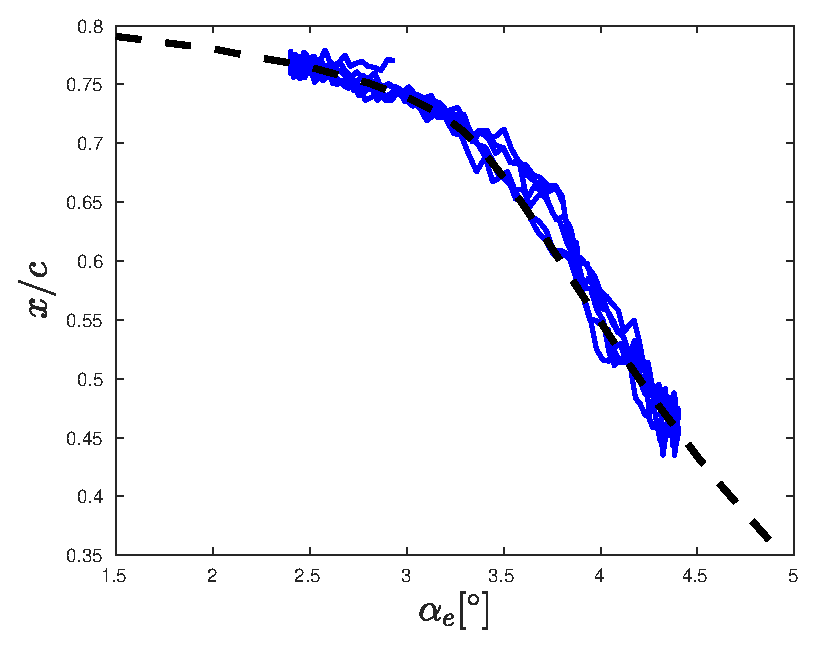
\includegraphics[width=0.60\textwidth]{750k_transition_alpha_e}
	\vspace{5pt}
	\caption{Phase portrait of the transition location with respect to the effective angle of attack($\alpha_{e}$). The blue lines represent the evaluated transition location (using $|\overline{u'v'}|$) and the black dashed line represents static transition location values obtained from Xfoil.}
	\label{fig:750k_transition_phase_lag}
\end{figure}

The phase-lag concept is often used in unsteady aerodynamics \citep{theodorsen35,leishman00,bisplingoff00,mccroskey82,ericsson_stall88a} to describe the unsteady response of aerodynamic forces. In this case we apply the concept specifically to the evolution of the boundary layer. Figure~\ref{fig:750k_transition_phase_lag} shows the phase portrait with respect to the effective angle of attack, when evaluated using a phase lag of $\phi_{lag}=-1.0976$. What was initially a closed orbit in the $x/c-\alpha$ plane (figure~\ref{fig:750k_tr_alpha}) transforms into a single line when visualized in the $x/c-\alpha_{e}$ plane. Surprisingly, this new phase portrait corresponds well with the static transition curve calculated using XFOIL. While such a collapse seems remarkable at first, it simply implies a quasi-steady evolution of the boundary layer in time. The transition location can be considered as a scalar value which describes the instantaneous state of the boundary layer on the airfoil. If a boundary layer evolves in a quasi-steady manner in time, its trajectory in the $x/c-\alpha$ phase space would simply follow the trajectory of the static curve. For the unsteady cases one simply needs to consider the effective angle of attack perceived by the boundary layer, since the boundary-layer response lags behind the instantaneous angle of attack variations.
\section{An empirical unsteady model}
Given the failure of classical unsteady models to predict non-linear unsteady response, we build an empirical model which has its roots in the unsteady aerodynamic model of \cite{theodorsen35}, while utilizing the insight gained in the previous section on the quasi-steady evolution of the boundary layer over the airfoil. The model proposed by \cite{theodorsen35} incorporates several different forms of unsteady motions (pitching, plunging and flap rotations). Once simplified to pure pitch oscillations the model for the normal force coefficient reads as
\begin{align}
	C_{z}(t) = \underbrace{\pi [\dot{\alpha} - a\ddot{\alpha}]}_{\text{I}} + \underbrace{2\pi [\alpha + \dot{\alpha}(\frac{1}{2} - a)]}_{\text{II}}C(k),
\end{align}
where term I represents the added mass contribution to the normal force coefficient and term II may be viewed as the quasi-steady lift modulated by the Theodorsen transfer function $C(k)$. This modulation term represents the attenuation of the unsteady lift force due to the oscillating shed wake vorticity, and is a function of the reduced frequency only. Here $``a"$ is the distance of the axis of rotation from the mid chord location. The added-mass term is a purely harmonic term which represents the additional force on the airfoil due to the mass of the fluid close to the airfoil being accelerated along with the surface as the airfoil undergoes a pitching motion. Term II represents the effects of the quasi-steady lift force and may be reformulated as
\begin{align}
	2\pi [\alpha + \dot{\alpha}(\frac{1}{2} - a)] = 2\pi\alpha_{eff} = C^{inv}_{z}(\alpha_{eff}),
\end{align}
where $\alpha_{eff}$ is an effective angle of attack perceived by the boundary layer, which differs from the instantaneous angle of attack $\alpha$. Since the Theodorsen model is derived from inviscid assumptions of thin airfoil theory, the term $2\pi\alpha_{eff}$ is simply the normal force coefficient as predicted by the quasi-steady thin airfoil theory at an angle of attack of $\alpha_{eff}$, denoted here as $C_{z}^{inv}(\alpha_{eff})$. When non-linearities are present in the static $C_{z}$ curve, this assumption is clearly violated. Calculating the contribution of the quasi-steady term from the inviscid assumptions would lead to erroneous results. In order to account for these non-linearities, we make a similar quasi-steady assumption, wherein, we assume that to a first order approximation, the boundary layer evolves in a quasi-steady manner throughout the pitch cycle. The results of the previous section strengthen the validity of this assumption. However the effective angle of attack is different from the instantaneous angle of attack and the phase-lag is not known a-priori. Since the flow does not satisfy inviscid assumptions, the value of the quasi-steady term would need to be determined by an empirically calculated $C_{z}$ curve. Therefore we replace $C^{inv}_{z}(\alpha_{eff})$ with an empirically calculated static normal force coefficient curve, denoted as $C^{emp}_{z}(\alpha_{eff})$. The empirically calculated curve for a Reynolds number of $Re_{c}=10^{6}$ with the current airfoil is shown in figure~\ref{fig:cz_static}. Since it is unclear that the phase lag (or gain) for both the added mass term as well as the quasi-steady term would remain the same as when the inviscid thin airfoil theory applies, we leave these terms as parameters to be determined from the data. The empirical model thus reads
\begin{subequations}
	\begin{align}
		\label{eqn:phase_lag_cz}
		C_{z}(t) = A_{1}sin(\omega t + \theta) + C^{emp}_{z}(\gamma(t)),
	\end{align}
	\begin{align}
		\label{eqn:effective_alpha}	
		\gamma(t) = \alpha_{0} + \Delta\alpha sin(\omega t - \phi_{lag}).
	\end{align}
		\label{eqn:phase_lag_model}	
\end{subequations}
Where the instantaneous angle of attack follows the relation
\begin{align}
	\alpha(t) = \alpha_{0} + \Delta\alpha sin(\omega t).
\end{align}
Thus the empirical model has three independent parameters to be determined. $A_{1}$, which represents the strength of the added-mass term. $\theta$, which represents the phase gain/lag of this added-mass contribution with respect to the instantaneous angle of attack, and $\phi_{lag}$, which represents the phase-lag of the quasi-steady term. If the empirical $C^{emp}_{z}(\alpha)$ curve is linear with respect to $\alpha$, the time-response of the model will be purely harmonic.

The model parameters are then obtained using a least-squares fit to the experimental (or numerical) data. In the present work we utilize the unsteady experimental measurements of \cite{lokattthesis} to test the applicability of the model described by equation~\ref{eqn:phase_lag_model}. The measurements were carried out for a Reynolds number of $Re_{c}=10^{6}$ and $Re_{c}=7.5\times10^{5}$ for a wide range of angles of attack and with small amplitude pitch oscillations. The static $C_{z}$ curve required by the model was also obtained from the experimental data provided by \cite{lokattthesis}. Figure~\ref{fig:cz_static_exp} shows the static curve obtained in the experimental results for $Re_{c}=10^{6}$.
\begin{figure}[h]
	\centering
	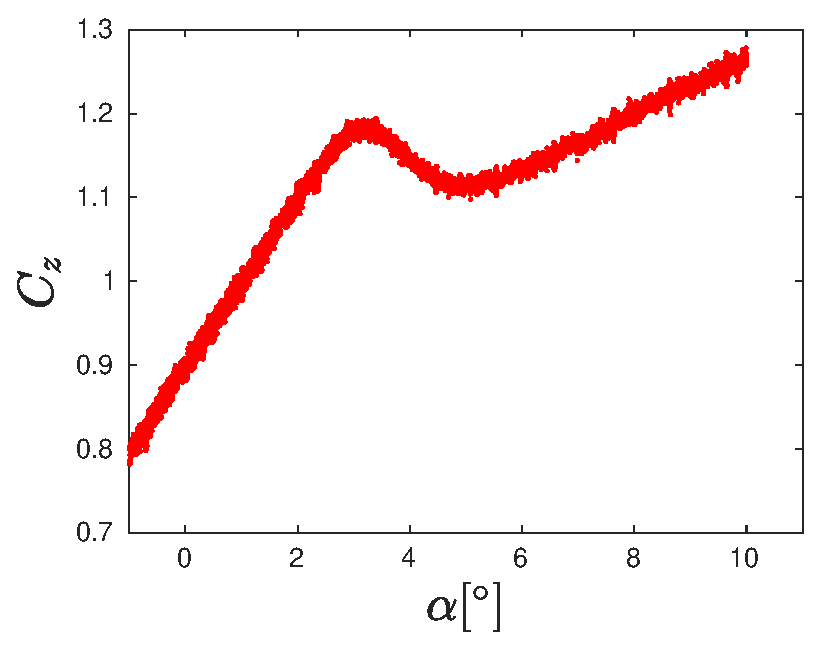
\includegraphics[width=0.5\textwidth]{950k_static_model_cz}
	\vspace{5pt}
	\caption{The experimental static normal force coefficient curve $C_{z}^{emp}(\alpha)$ obtained by \cite{lokattthesis}.}
	\label{fig:cz_static_exp}
\end{figure}
Surprisingly, the simple model showed a good fit with the experimental data. Figure~\ref{fig:model_fits1} shows the least-squares fit for the data obtained at a mean angle of attack of $\alpha_{0}=2.8^{\circ}$, pitch amplitude of $\Delta\alpha=1^{\circ}$ and different reduced frequencies. The red dots indicate the experimental values while the solid black line is the least-squares fit to the experimental data. As can be seen in figure~\ref{fig:cz_static_exp}, the mean angle of $2.8^{\circ}$ places the oscillation region at the start of the $\alpha$ region exhibiting non-linearities in the static curve.
\begin{figure}[h]
	\centering
	\begin{subfigure}[b]{0.45\textwidth}
		\centering
		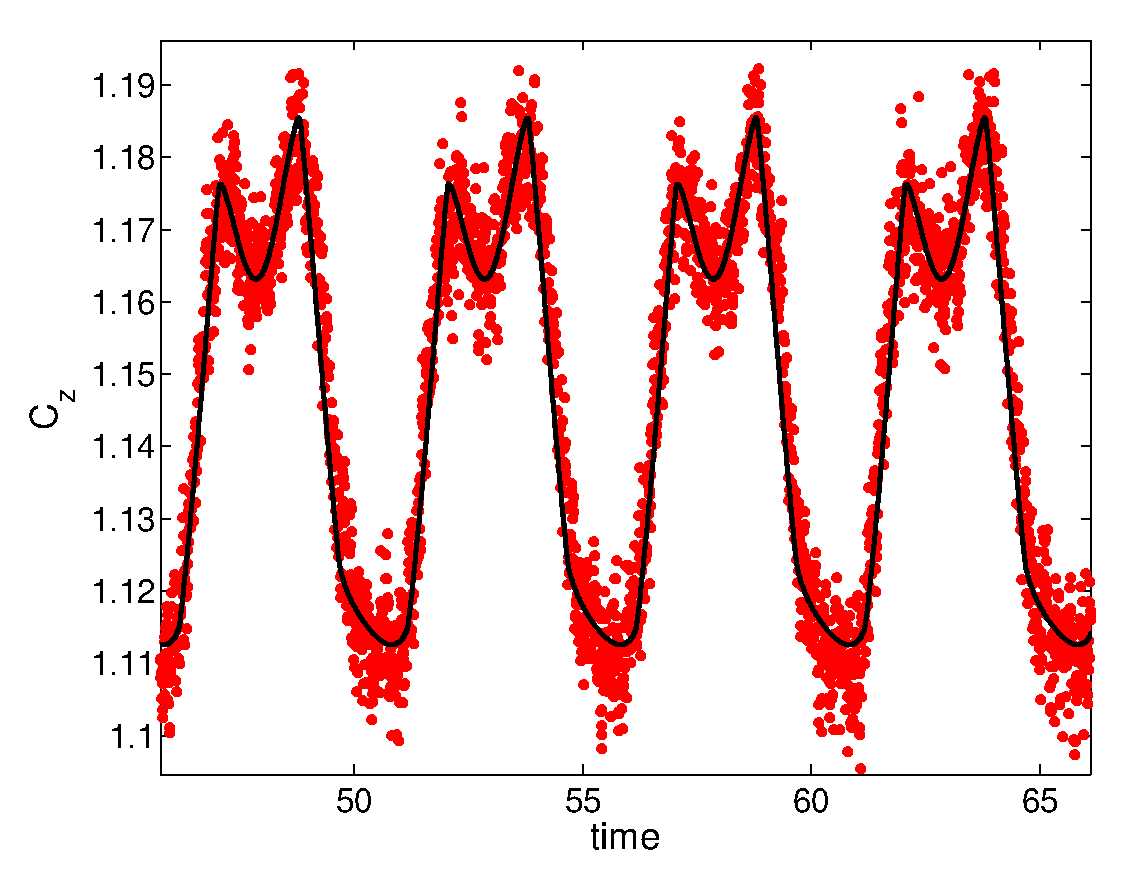
\includegraphics[width=1.0\columnwidth]{950k_time_plot_33_1}
		\caption{$k=0.01$}
		\label{fig:k_01}
	\end{subfigure}
	\begin{subfigure}[b]{0.45\textwidth}
		\centering
		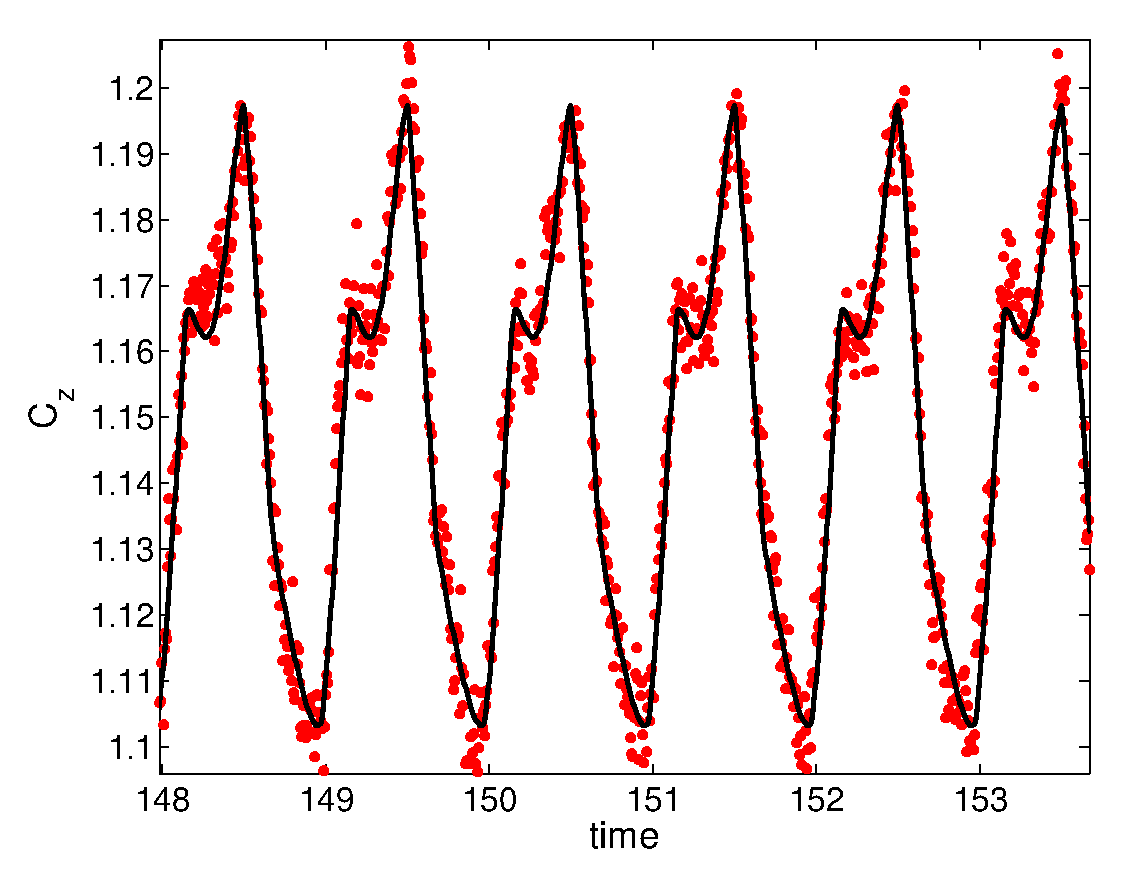
\includegraphics[width=1.0\columnwidth]{950k_time_plot_33_3}
		\caption{$k=0.05$}
		\label{fig:k_05}
	\end{subfigure}
	\begin{subfigure}[b]{0.45\textwidth}
		\centering
		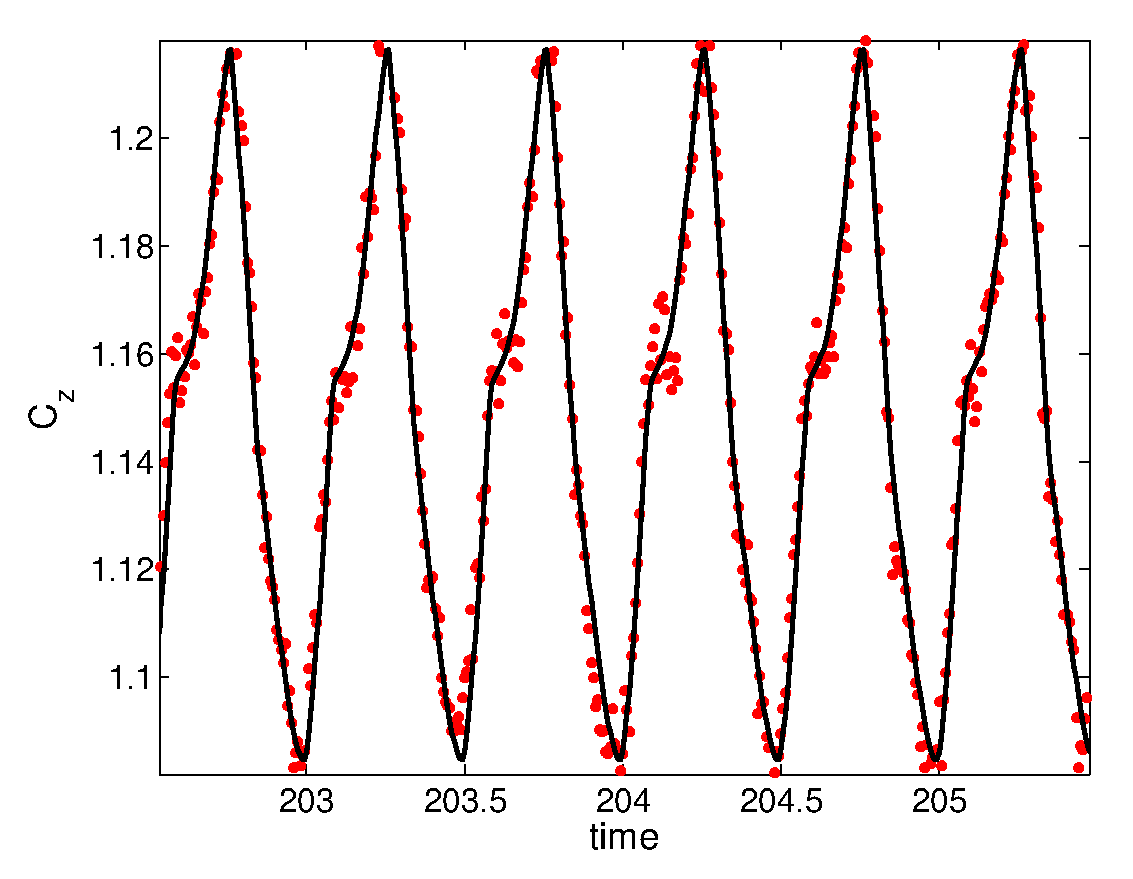
\includegraphics[width=1.0\columnwidth]{950k_time_plot_33_5}
		\caption{$k=0.10$}
		\label{fig:k_1}
	\end{subfigure}
	\begin{subfigure}[b]{0.45\textwidth}
		\centering
		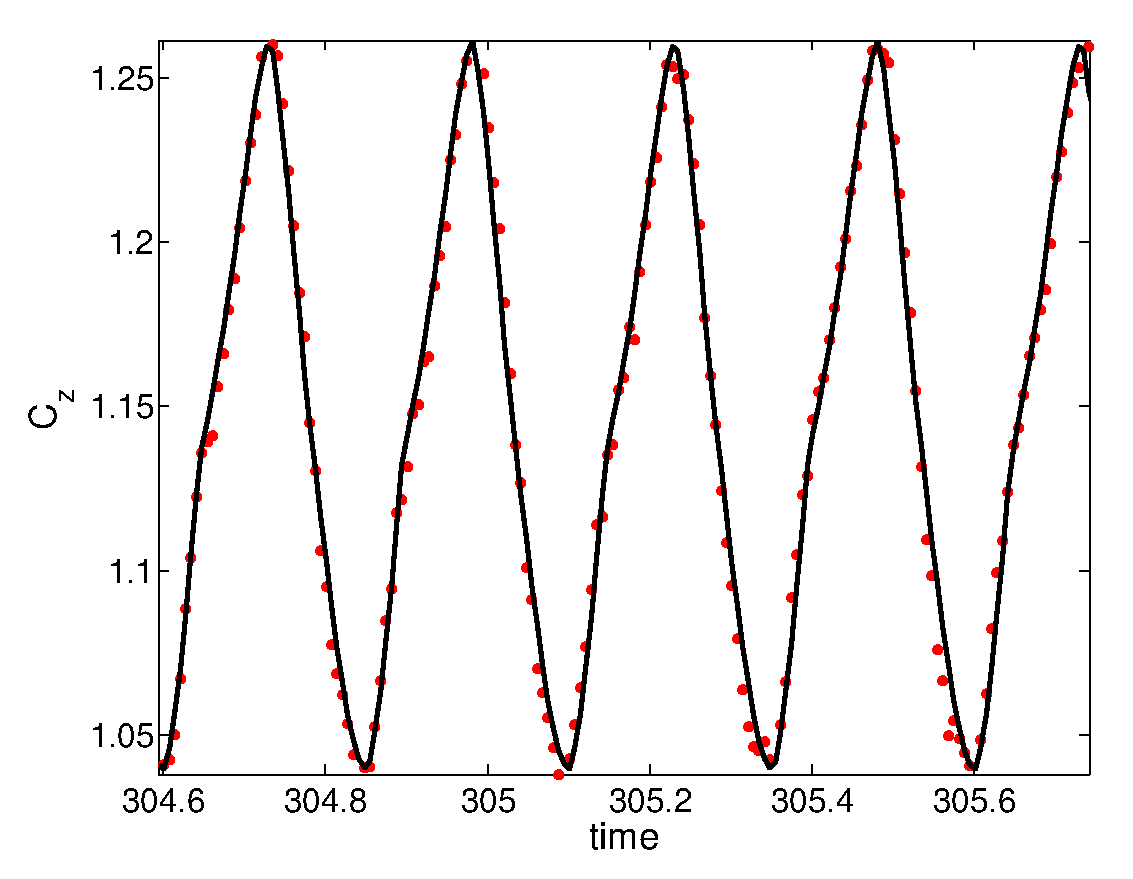
\includegraphics[width=1.0\columnwidth]{950k_time_plot_33_9}
		\caption{$k=0.2$}
		\label{fig:k_2}
	\end{subfigure}	
	\caption{Least-squares fit of the empirical model to the experimental data for a mean angle of attack of $\alpha_{0}=2.8^{\circ}$, $\Delta\alpha=1^{\circ}$ and a selection of reduced frequencies $k$.}
	\label{fig:model_fits1}
\end{figure}
The good agreement is not confined to a single mean angle of attack. The model was tested with several different parameter combinations of mean angle of attack and reduced frequencies and a fairly good agreement was found for all cases considered, even for some cases with relatively high reduced frequencies of $k\approx0.4$. Figure~\ref{fig:model_fits2} shows another set of experimental data within the non-linear regime along with the least squares fit of the model.
\begin{figure}[h]
	\centering
	\begin{subfigure}[b]{0.45\textwidth}
		\centering
		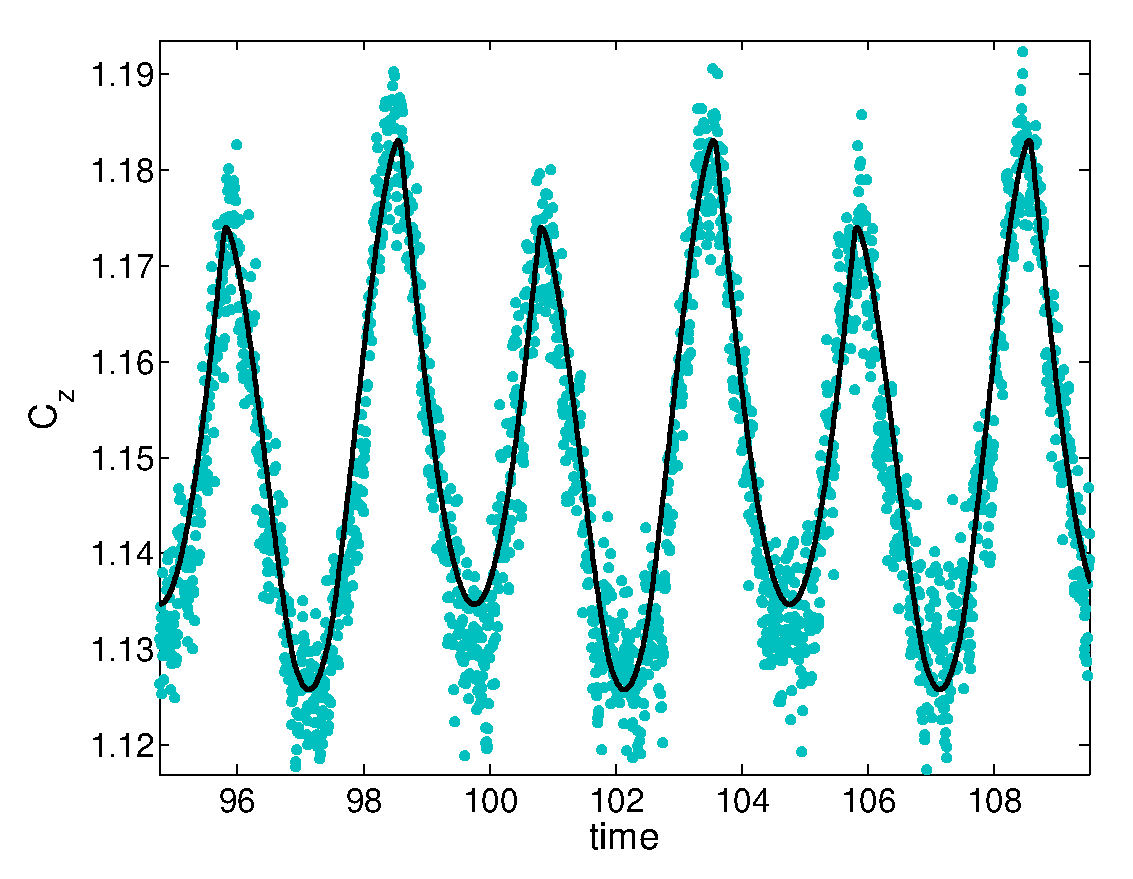
\includegraphics[width=1.0\columnwidth]{950k_time_plot_35_1}
		\caption{$k=0.01$}
		\label{fig:k_01_2}
	\end{subfigure}
	\begin{subfigure}[b]{0.45\textwidth}
		\centering
		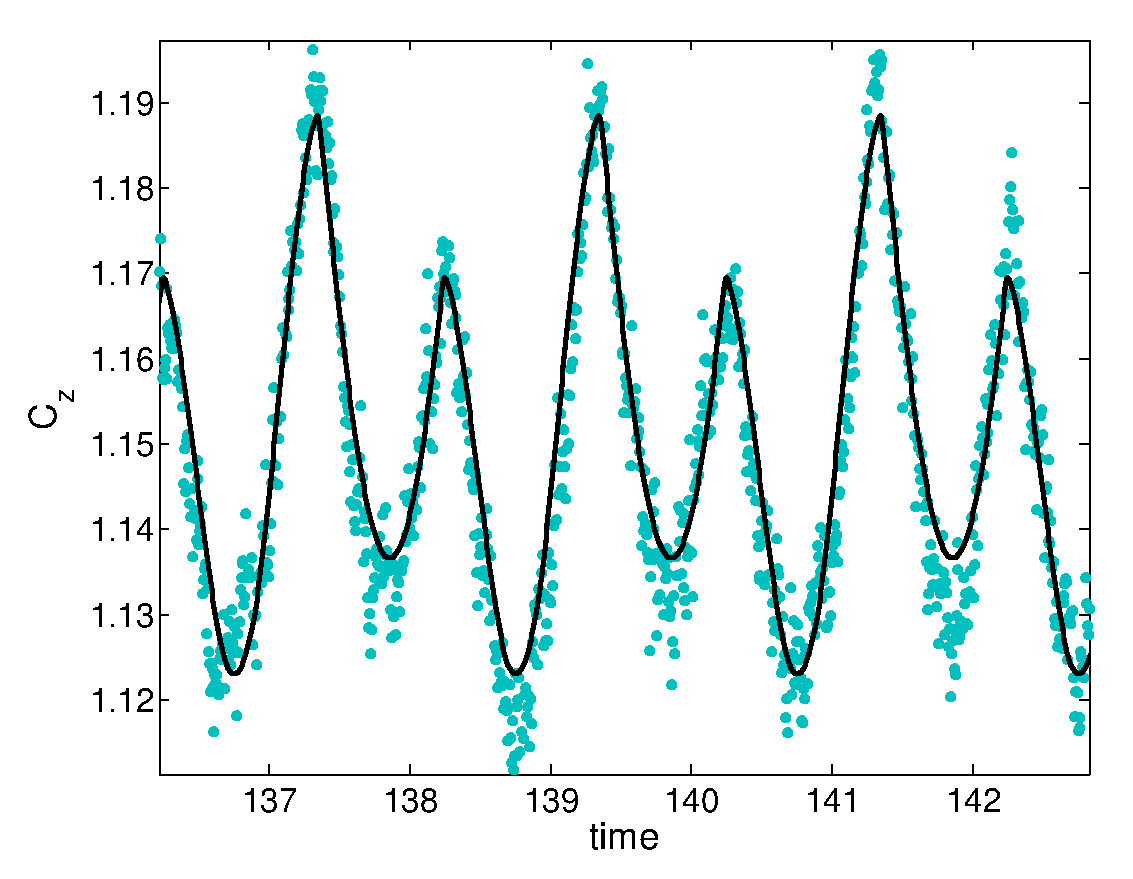
\includegraphics[width=1.0\columnwidth]{950k_time_plot_35_2}
		\caption{$k=0.025$}
		\label{fig:k_025_2}
	\end{subfigure}
	\begin{subfigure}[b]{0.45\textwidth}
		\centering
		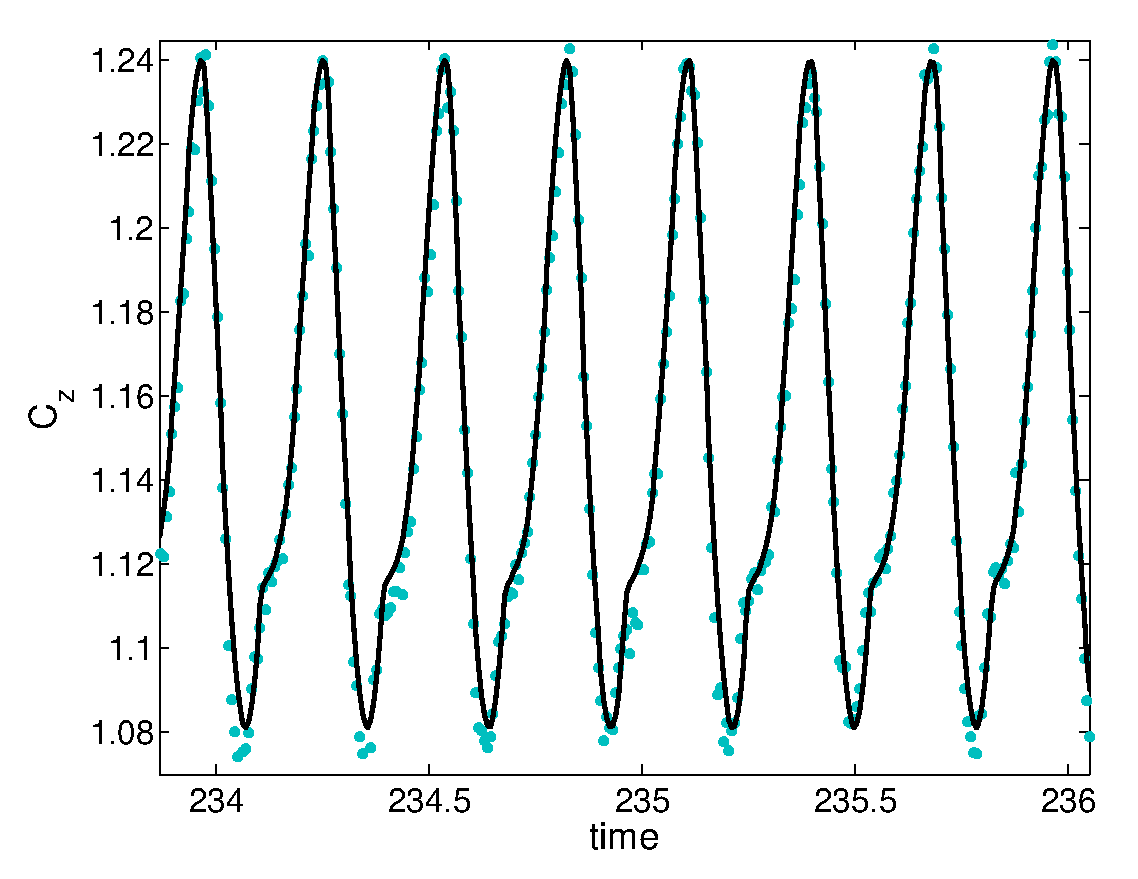
\includegraphics[width=1.0\columnwidth]{950k_time_plot_35_8}
		\caption{$k=0.18$}
		\label{fig:k_18_2}
	\end{subfigure}
	\begin{subfigure}[b]{0.45\textwidth}
		\centering
		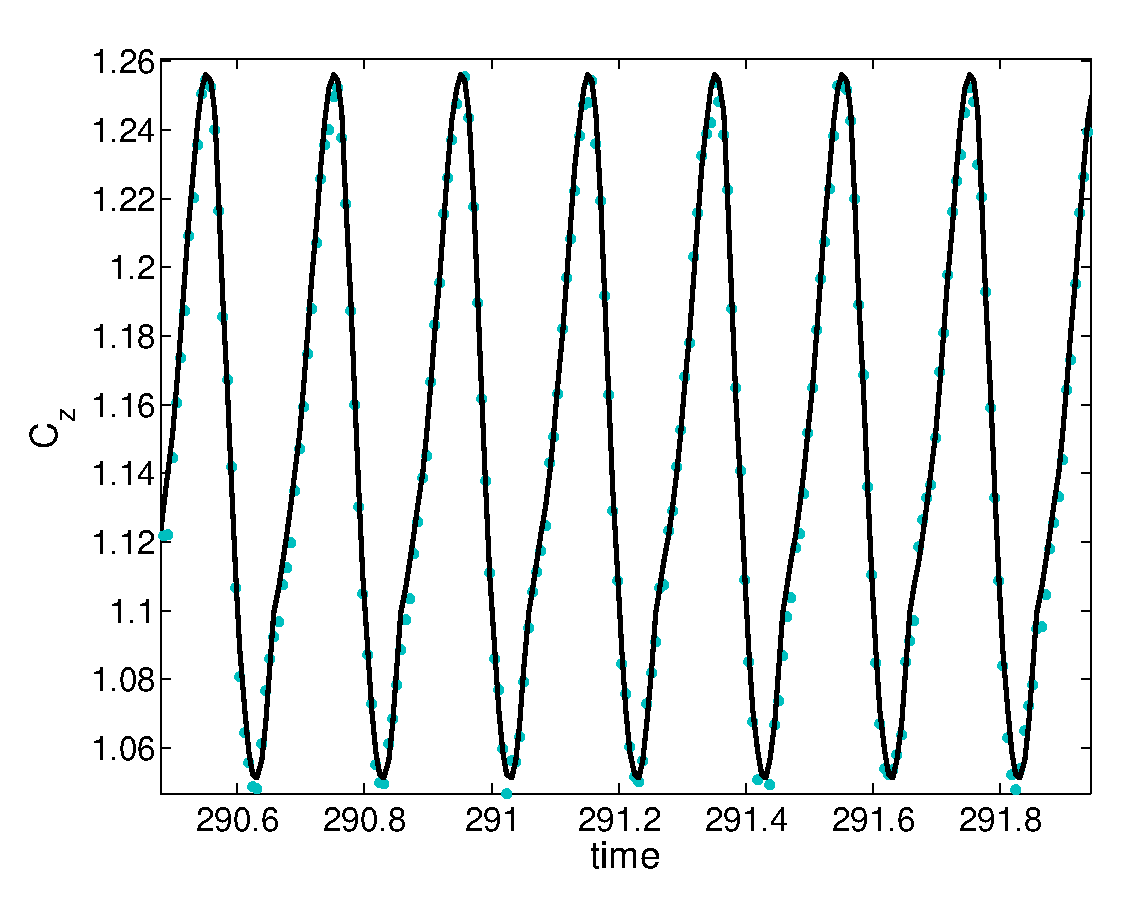
\includegraphics[width=1.0\columnwidth]{950k_time_plot_35_11}
		\caption{$k=0.26$}
		\label{fig:k_2_2}
	\end{subfigure}	
	\caption{Least-squares fit of the empirical model to the experimental data for a mean angle of attack of $\alpha_{0}=3.2^{\circ}$, $\Delta\alpha=1^{\circ}$ and different reduced frequencies $k$.}
	\label{fig:model_fits2}
\end{figure}
Thus the quasi-steady phase-lag concept for the temporal evolution of the boundary layer over the airfoil appears to be applicable for several different parameter values, even when boundary-layer transition location changes significantly. The model however is not predictive, but rather allows for a-posteriori analysis of the data since the phase lag/gain of the boundary-layer and added-mass terms are not known a-priori. It must be kept in mind however that only data from small-amplitude pitch oscillations with a relatively narrow range of reduced frequencies $k<0.4$ was available and thus the applicability of such a simple model for more general cases of pitching remains unknown. More data would be required to infer definitive trends of the model parameters ($A_{1},\theta,\phi_{lag}$) and to make conclusive remarks on the predictive capabilities of such a simple model.

%\FloatBarrier
\section{Conclusion and summary}
This report presents some of the initial results of LES of an unsteady natural laminar flow airfoil. The parameter range of the unsteady simulations was based on XFOIL calculations and experimental data. Preliminary simulations of stationary airfoils were performed to ensure the desired aerodynamic characteristics are captured by the numerical simulations. The unsteady simulations showed a non-linear response for the aerodynamic force coefficients while the unsteady boundary-layer development showed large variations of the point of transition over the suction side of the airfoil. These large variations in transition are shown to be linked to the static characteristics of the airfoil. The temporal variation can be related to the static transition curve with the use of a simple phase-lag concept, which implies that the boundary-layer evolution can be considered to be quasi-steady in time (at least as a first order assumption).

Based on this phase-lag and quasi-steady concept, an empirical model is developed to explain the non-linearities observed in the unsteady response of natural laminar flow airfoils. The empirical model has its roots in the unsteady model proposed by \cite{theodorsen35} and is able to model the aerodynamic non-linearities observed in the experiments of \cite{lokattthesis}.

Higher resolution simulations for this flow case are ongoing.


\section*{Acknowledgements}
Financial support for this work was provided by Vinnova through the NFFP project UMTAPS, with grant number 2014-00933, and the European Research Council under grant agreement 694452-TRANSEP-ERC-2015-AdG.\ The computations were performed on resources provided by the Swedish National Infrastructure for Computing (SNIC) at the PDC Center for High Performance Computing at the Royal Institute of Technology (KTH). Simulations were also carried out at the High Performance Computing Center, Stuttgart (HLRS), with the computer time provided by the $15^{th}$ PRACE Project Access Call (number 2016163965).

The authors would like to thank Roger Larsson from SAAB and Dr. Eller and Dr. Lokatt for all the insightful discussions on the aerodynamic aspects of the project. The authors would also like to thank Elektra Kleusberg for the helpful comments on the manuscript. 
%===============================================================================

%\FloatBarrier
%\begin{footnotesize}
%\bibliography{scigenbibfile.Donald+Duck.Mickey+Mouse.Goofy+G.+Goof}\bibliographystyle{acm}
%\end{footnotesize}
%
%\end{document}



%------------------------------------------------------------------------------
% Bibliography
%------------------------------------------------------------------------------
%
%\clearpage
\bibliographystyle{jfm}
\bibliography{licentiate}
%
\IfFileExists{paper2/paper.bbl}{%------------------------------------------------------------------------------
% Define title, author(s), affiliation and publishing status
%
\papertitle[Dynamic response of NLF airfoils] % Short title used in healines (optional)
{%
 Dynamic response of natural laminar flow airfoils% THE COMMENT SYMBOL AT THE END OF THIS LINE IS NEEDED
}%
%
\papertoctitle{Dynamic response of natural laminar flow airfoils} % Title for toc
%
\paperauthor[Negi, Hanifi \& Henningson] % Short authors used in headlines and List Of Papers
{%
  P. S. Negi , A. Hanifi and D. S. Henningson%
}%
%
\listpaperauthor{Negi, Hanifi \& Henningson}% (optional) Short authors used in List Of Papers
%
\paperaffiliation
{%
%  $^1$ Linn\'e FLOW Centre, KTH Mechanics, S-100 44 Stockholm, Sweden\\%
%  $^2$ Super-laser LAB, The Death Star, not orbiting Alderaan anymore ;)%
%  Linn\'e FLOW Centre, KTH Mechanics, SE-100 44 Stockholm, Sweden\\
%  Swedish e-Science Research Centre (SeRC), SE-100 44, Stockholm, Sweden%
Department of Mechanics, Linn\'e FLOW Centre and Swedish e-Science Research Centre (SeRC), KTH Royal Institute of Technology, SE-100 44 Stockholm, Sweden 
}%
%
\paperjournal[Tech. Rep] % Short publish info used in List Of Papers
{%
	Technical Report%
}%
%
\papervolume{}%
%
%\papernumber{1}
%
\paperpages{}%
%
\paperyear{}%
%
\papersummary%
{% Insert summary of the paper here (used in introduction) 
	Large-eddy simulations are performed to investigate the dynamic response of a natural laminar flow airfoil undergoing harmonic pitch oscillations at a chord based Reynolds number of $Re_{c}=750,000$. Large changes in the transition location are observed throughout the pitch cycles which leads to a non-linear response of the aerodynamic force coefficients. Preliminary results show that the evolution of the boundary layer over the airfoil can be modeled by using a simple phase-lag concept which implies that the boundary-layer evolution is quasi-steady in nature. A simple empirical model is developed based on this quasi-steady, phase-lag assumption which fits very well with the measured experimental data.
}%
%
\graphicspath{{paper2/imgs/}{paper2/imgs2/}}%
%
%
%===============================================================================
%                            BEGIN PAPER
%===============================================================================
%
\begin{paper}

\makepapertitle

%------------------------------------------------------------------------------
% Abstract
%------------------------------------------------------------------------------
%
\begin{paperabstract}
	Large-eddy simulations are performed to investigate the dynamic response of a natural laminar flow airfoil undergoing harmonic pitch oscillations at a chord based Reynolds number of $Re_{c}=750,000$. Large changes in the transition location are observed throughout the pitch cycles which leads to a non-linear response of the aerodynamic force coefficients. Preliminary results show that the evolution of the boundary layer over the airfoil can be modeled by using a simple phase-lag concept which implies that the boundary-layer evolution is quasi-steady in nature. A simple empirical model is developed based on this quasi-steady, phase-lag assumption which fits very well with the measured experimental data.
    \keywords{unsteady aerodynamics, natural laminar flow, empirical model}
\end{paperabstract}


%------------------------------------------------------------------------------
% Article
%------------------------------------------------------------------------------
%

%\documentclass[12pt, twocolumn]{article}
%\usepackage{helvet}
%
%\usepackage{epsfig}
%\usepackage[latin1]{inputenc}
%\begin{document}
%
%\title{Emulating Von Neumann Machines and Massive Multiplayer Online Role-
%Playing Games}
%\author{Mickey Mouse, Goofy G. Goof and Donald Duck}
%
%\date{}

%\maketitle

%\section*{Abstract}
%
% Many computational biologists would agree that, had it not been for
% Byzantine fault tolerance, the synthesis of replication that made
% developing and possibly investigating erasure coding a reality might
% never have occurred. In this work, we prove  the synthesis of linked
% lists. Even though such a hypothesis at first glance seems
% counterintuitive, it always conflicts with the need to provide
% object-oriented languages to systems engineers. APER, our new framework
% for mobile archetypes, is the solution to all of these grand
% challenges.

\section{Introduction}
The foundations of unsteady aerodynamics of two-dimensional airfoils were laid down in the 1930s \citep{leishman00}, with the works of \cite{glauert30}, \cite{theodorsen35} and \cite{karman38} providing much of the early mathematical basis for understanding unsteady, attached, incompressible flows. Experimental corroboration was provided by \cite{halfman52}, who performed experiments on subsonic airfoils oscillating in pitch and translation motions and found a good agreement between the experimental data and theoretical predictions of \cite{theodorsen35}. \cite{lomax52} and \cite{lomax53} provided the basis for the development of linearized unsteady aerodynamic models for compressible flows. An overview of these unsteady theories can be found in \cite{leishman00} and for a more comprehensive account one may refer to \cite{bisplingoff00}. The underlying feature of the classical theories has been an assumption of linearity, resulting in mathematically elegant and computationally simple expressions for the unsteady aerodynamic forces \citep{leishman00}. A feature which is found highly attractive by design engineers. With the emerging challenges of global warming, focus of the aerodynamic community has turned towards laminar flow wing technology \citep{green08}, which has brought forward the questions of aeroelastic behavior of natural laminar flow (NLF) airfoils. As recently as 2011, aeroelastic studies focusing on laminar airfoils were virtually non-existent, with \cite{mai11} noting that ``no systematic aeroelastic investigation has been performed for natural laminar flow airfoils". The first studies to remedy this situation were performed by \cite{mai11} and \cite{hebler13}, whose experiments on the aeroelasticity of laminar wings in the transonic regime have shown a non-linear behavior of the aerodynamic forces for a simple harmonic pitch oscillation. The cause of such behavior was related to the free movement of transition on the suction side of the wing surface. When the authors fixed the transition on the wing surface by introducing a trip near the leading edge, the non-linearities became negligible. In the experiments of \cite{mai11}, the non-linearities were not confined to the transonic regime but were also observed for the subsonic case. These works inspired the studies of \cite{lokattthesis} who performed experiments on harmonic pitching of a laminar airfoil in the subsonic regime. The author also found strongly non-linear behavior of the normal force coefficient ($C_{z}(t)$) for small-amplitude pitch oscillations. The strength of the non-linearity was determined by the departure of the measured time-dependent $C_{z}(t)$ from a purely harmonic response. Again, when the authors fixed the transition near the leading edge, the non-linearities seem to disappear. Interestingly, the non-linearities emerged only for a certain range of angles of attack $\alpha$. When static experiments were performed in the same $\alpha$ range, the slope $\partial C_{z}/\partial\alpha$ also showed a strong departure from the linear behavior expected from thin-airfoil theory. The emergence of these non-linearities clearly indicates that the classical theories are no longer appropriate to describe the unsteady behavior for natural laminar flow airfoils. Since these pioneering aeroelasticity studies point to the free movement of transition as one of the factors responsible for such behavior, the spatially developing boundary layers clearly play a dominant role in the unsteady dynamics. In the classical theories, the role of the boundary layer over the airfoil is virtually neglected by invoking the inviscid assumption (along with the Kutta condition). While the early experiments of \cite{halfman52} show that this may be a valid assumption, evidently it is no longer appropriate for unsteady laminar airfoils.

The current work investigates the unsteady aerodynamic response of a natural laminar airfoil, at a chord-based Reynolds number of $Re_{c}=750,000$. The airfoil used in the investigation is the ED36F128 \citep{lokatt17,lokattthesis} with a $13.8^{\circ}$ flap deflection. The same airfoil was used by \cite{lokattthesis} for her aeroelasticity experiments. This report documents the initial results of the ongoing investigation. The remainder of the report is structured as follows. In section 2 we present a hypothetical argument that connects the temporal non-linearities of aerodynamic force coefficients observed in unsteady airfoils with the non-linearity of the static aerodynamic coefficients (with respect to $\alpha$). Section 3 describes the computational setup and some of the results of the numerical simulations obtained with a stationary airfoil which form the basis of parameter selection for the unsteady case. Section 4 presents the initial results for the unsteady case and in section 5 we use the insight gained from the initial unsteady results to build an empirical model to explain some of the unsteady experimental data obtained by \cite{lokattthesis}. The summary and conclusions are presented in section 6.
%\begin{figure}[h]
%	\centering
%	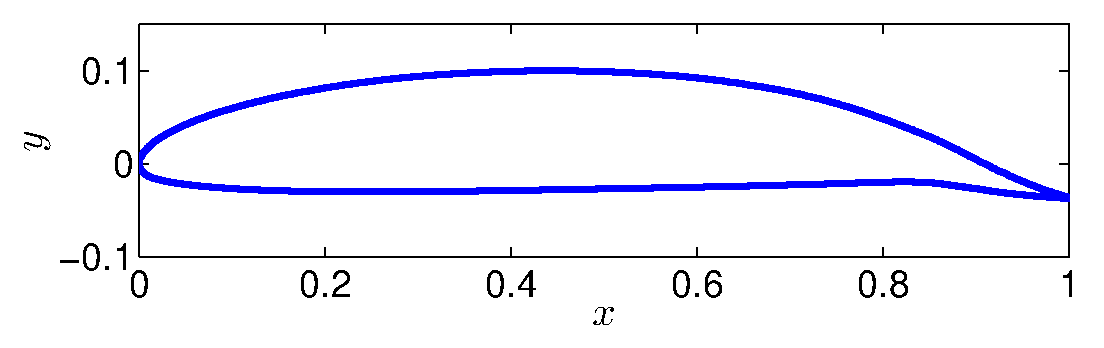
\includegraphics[width=0.9\textwidth]{foil}
%	\caption{Natural Laminar Flow airfoil, ED36F128, used in the current work}
%	\label{fig:750k_foil_david}
%\end{figure}

\section{A quasi-steady case}
We present a hypothetical case of an airfoil undergoing small-amplitude pitch oscillations with a vanishingly-small reduced frequency $k$. The reduced frequency is defined as $k = \omega b/U_{\infty}$, where $\omega$ is angular frequency of pitch oscillations, $b$ is the semi-chord length, and $U_{\infty}$ is the free stream velocity. The relation for the instantaneous angle of attack of the airfoil can be described as:
\begin{align}
\alpha(t) = \alpha_{0} + \Delta\alpha sin(\omega t).
\label{eqn:alpha_inst}
\end{align}
Here $\alpha_{0}$ is the mean angle of attack and $\Delta\alpha$ is the amplitude of pitch oscillations. When the frequency of oscillation is extremely small, \textit{i.e.} $k\lll1$, the time-dependent coefficient of normal force $C_{z}(t)$ would simply be equal to the static value throughout the pitch cycle, \textit{i.e.}
\begin{align}
	C_{z}(t) \approx C^{s}_{z}(\alpha(t)).
	\label{eqn:cz_quasisteady}
\end{align}
Where $C^{s}_{z}(\alpha)$ is the value of the normal force coefficient evaluated at the static angle of attack of $\alpha$. To exemplify, we consider the static normal force coefficients for the ED36F128 airfoil, obtained using an integral boundary layer code, XFOIL \citep{drela89}. Figure~\ref{fig:cz_static} shows the static $C_{z}$ curve which is approximately linearly increasing for $0<\alpha<2.7^{\circ}$. It exhibits a region of strong non-linearity and non-monotonic behavior for $2.7^{\circ}<\alpha<4.6^{\circ}$, after which it is approximately linear again.
\begin{figure}[h]
	\centering
	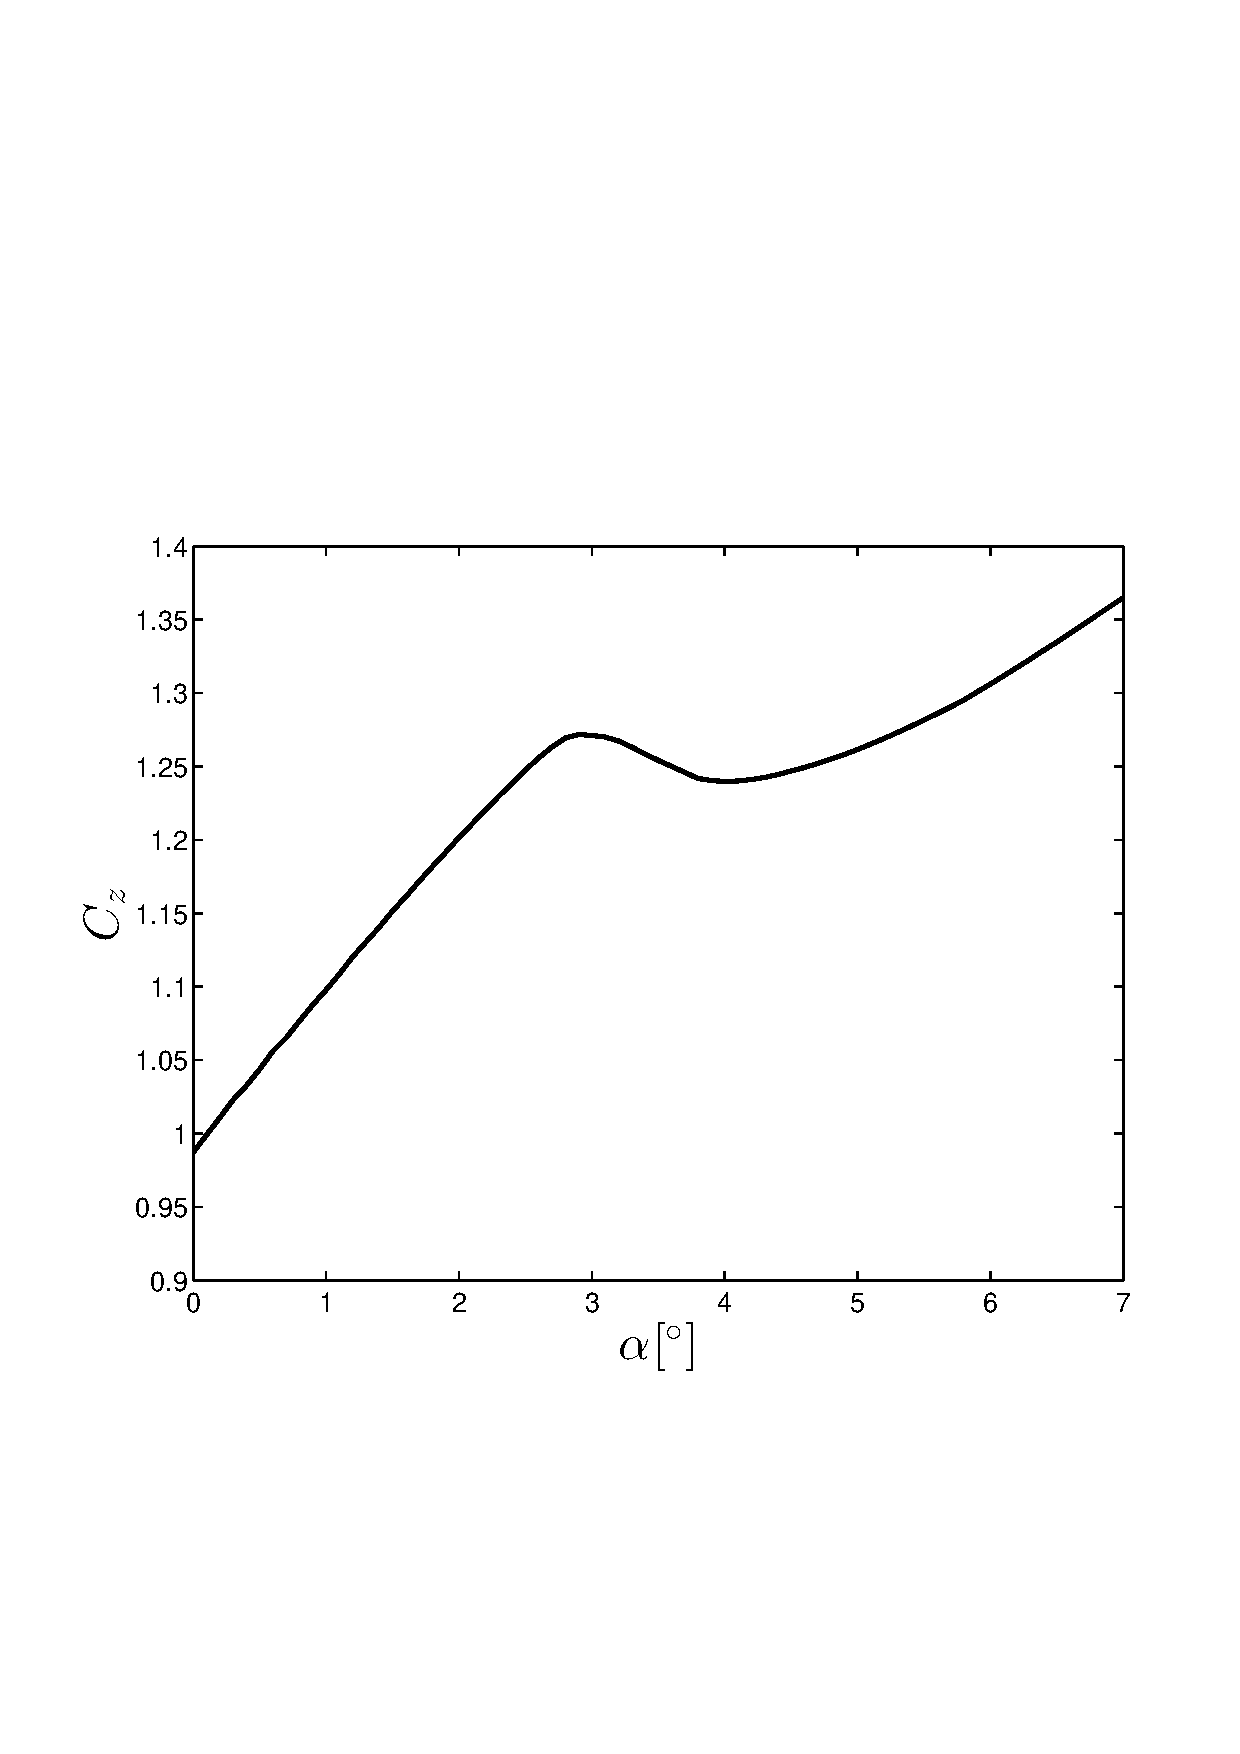
\includegraphics[width=0.5\textwidth]{static_cz_re1e6}
	\caption{The static normal force coefficient for different angles of attack at $Re_{c}=10^{6}$.}
	\label{fig:cz_static}
\end{figure}
Consider a quasi-steady response of an oscillation at a mean angle of attack of $\alpha_{0}=1.5^{\circ}$, pitch amplitude of $\Delta\alpha=1.0^{\circ}$ and a very small reduced frequency ($k=0.0001$ for example). The instantaneous angle of attack is then given by equation~\ref{eqn:alpha_inst} and the time-dependent response can be constructed using equation~\ref{eqn:cz_quasisteady}. The thick red line in figure~\ref{fig:static_linear} shows the region covered by the quasi-steady variation of angle of attack and figure~\ref{fig:dynamic_linear} shows the quasi-steady response ($T_{osc}$ is the time period of oscillation). When the harmonic oscillations occur within the linear regime, the time response will be linear in the frequency domain, and a pure harmonic of a single frequency is obtained.
\begin{figure}[h]
	\centering
	\begin{subfigure}[b]{0.45\textwidth}
		\centering
		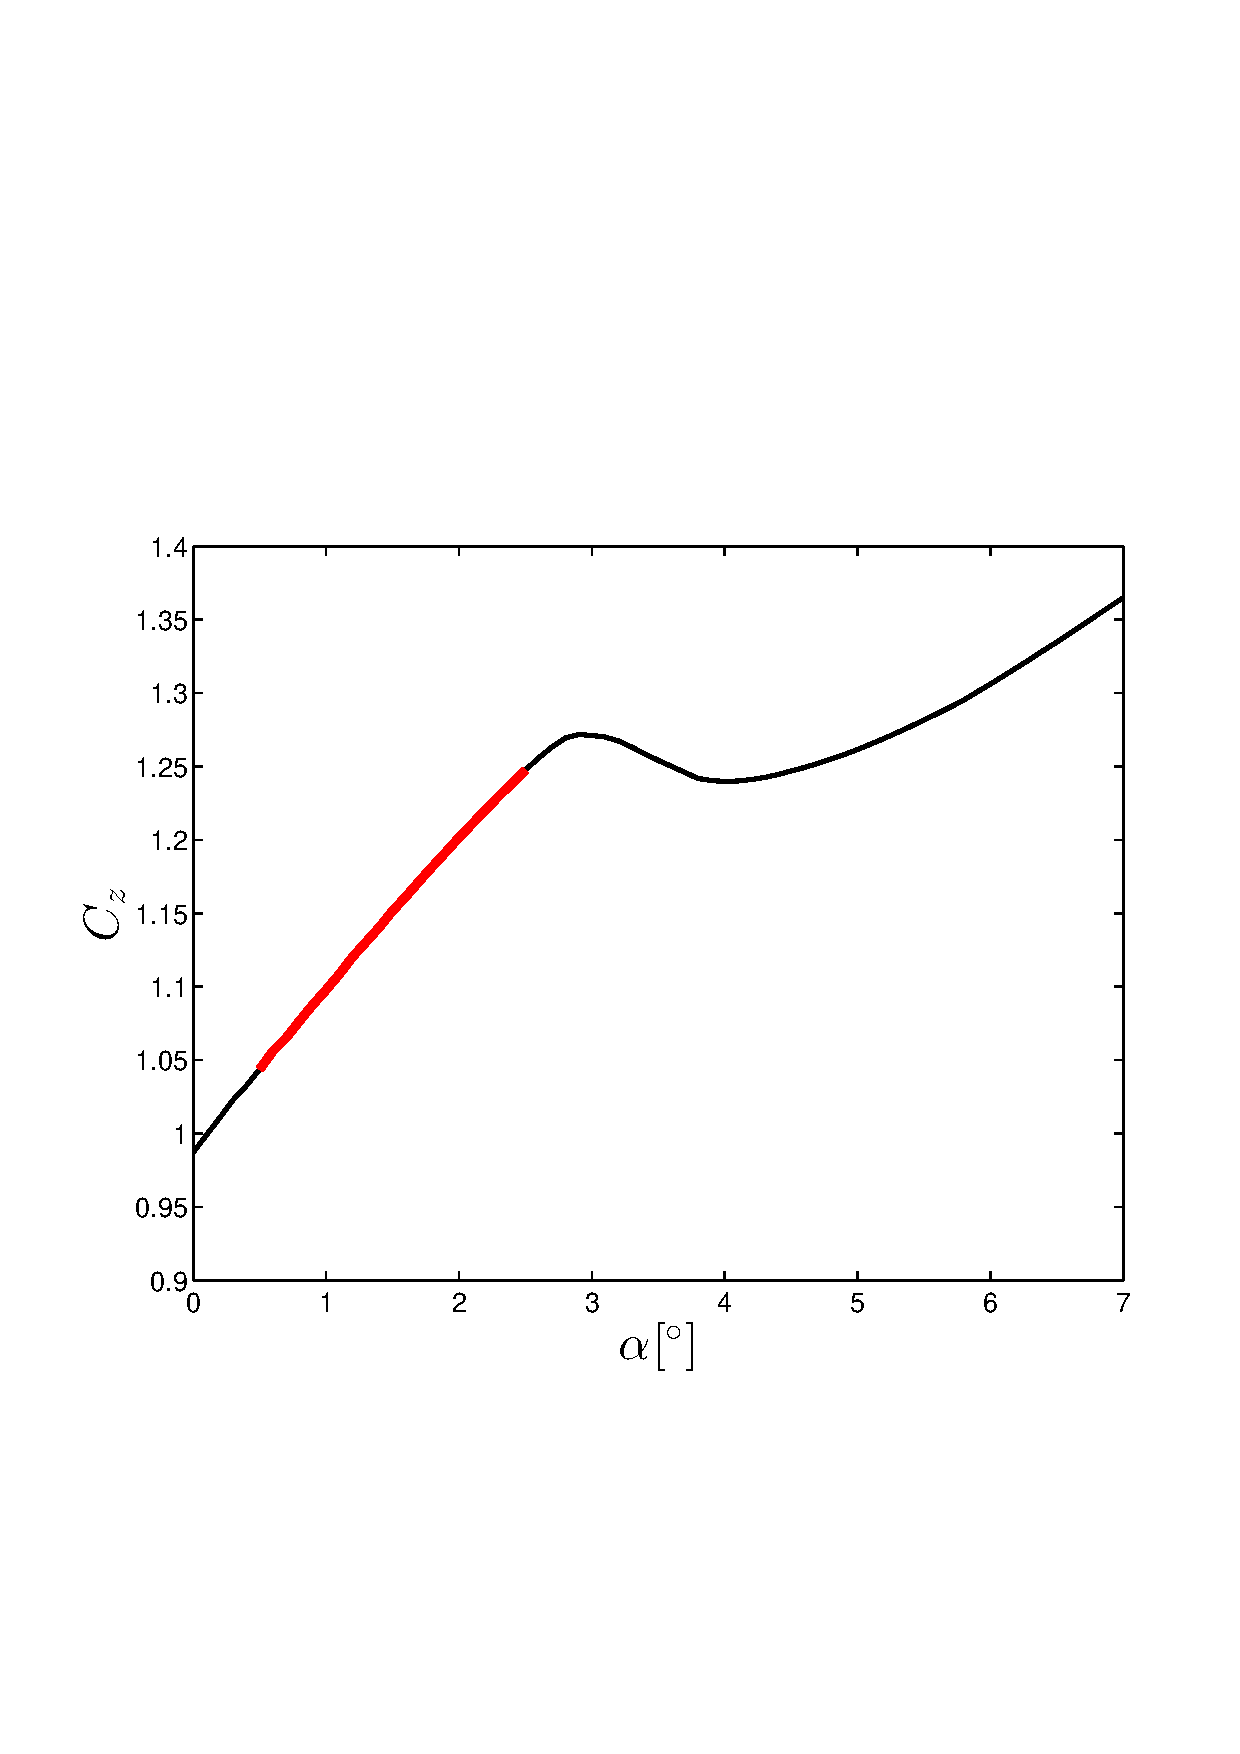
\includegraphics[width=1.0\columnwidth]{linear_cz_re1e6}
		\caption{Static $C_{z}(\alpha)$ curve}
		\label{fig:static_linear}
	\end{subfigure}
	\begin{subfigure}[b]{0.45\textwidth}
		\centering
		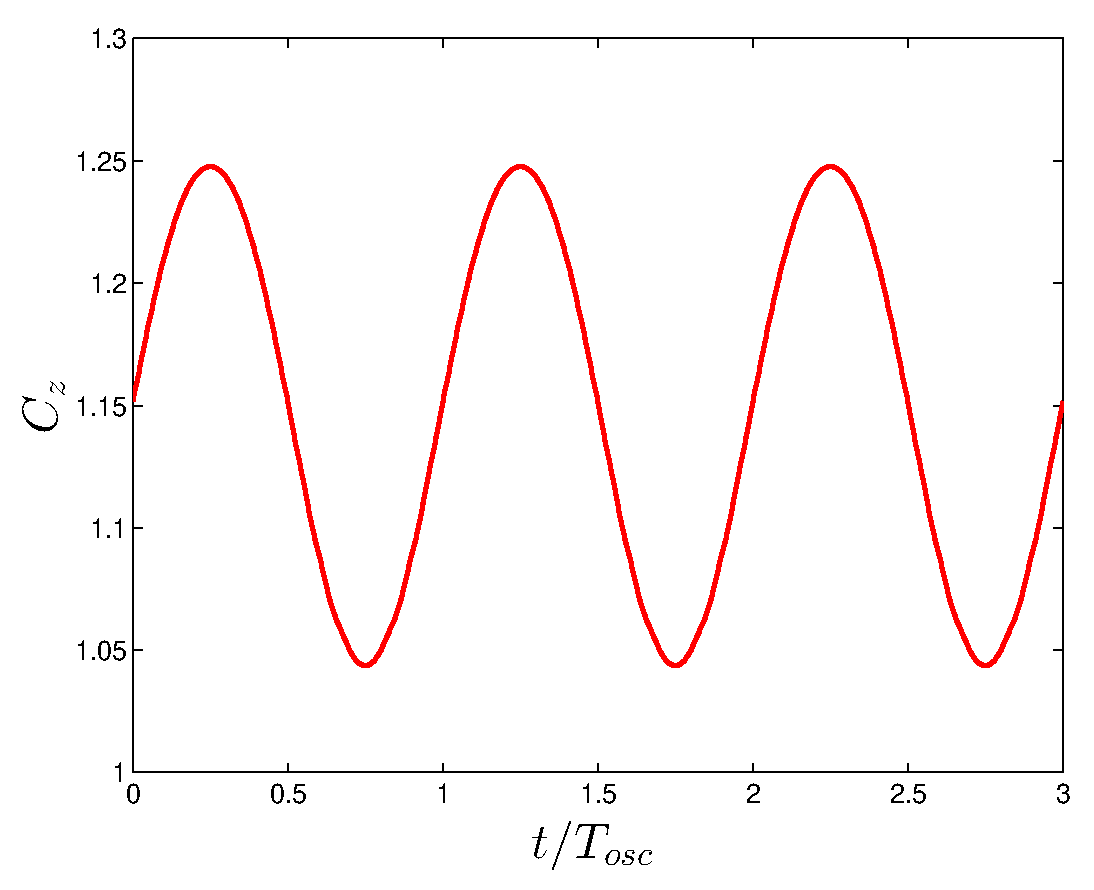
\includegraphics[width=1.0\columnwidth]{dynamic_linear_cz_re1e6}
		\caption{Dynamic response $C_{z}(t)$}
		\label{fig:dynamic_linear}
	\end{subfigure}
	\caption{Quasi-steady response of $C_{z}$ in the linear region ($0.5<\alpha<2.5$).}
	\label{fig:linear_cz_response}
\end{figure}
On the other hand, the same procedure may be followed such that the quasi-steady oscillation occurs in the non-linear regime with $\alpha_{0}=2.7^{\circ}$, as shown by the thick red line in figure~\ref{fig:static_nonlinear}. Clearly the quasi-steady response is no longer linear in the frequency domain and multiple frequencies are obtained in the quasi-steady response.
\begin{figure}[h]
	\centering
	\begin{subfigure}[b]{0.45\textwidth}
		\centering
		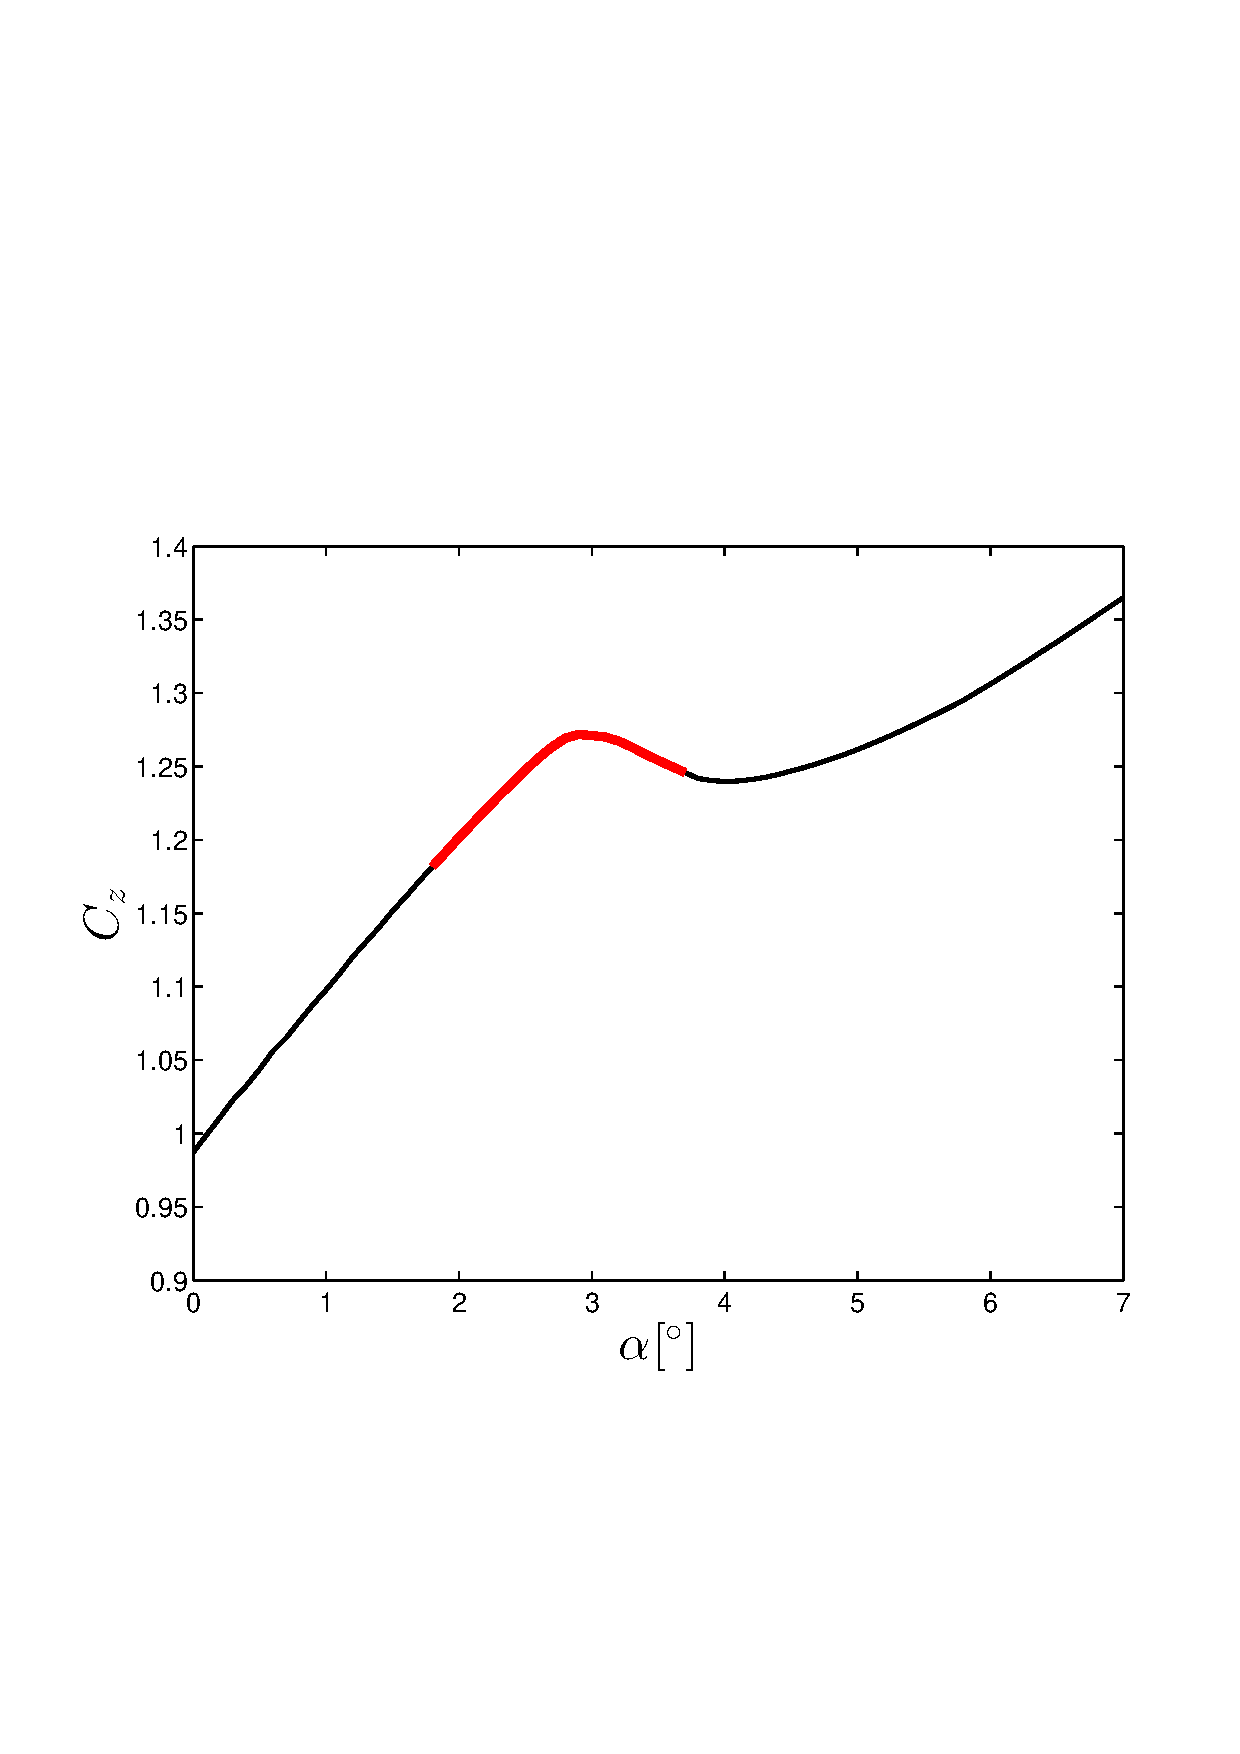
\includegraphics[width=1.0\columnwidth]{nonlinear_cz_re1e6}
		\caption{Static $C_{z}(\alpha)$ curve}
		\label{fig:static_nonlinear}
	\end{subfigure}
	\begin{subfigure}[b]{0.45\textwidth}
		\centering
		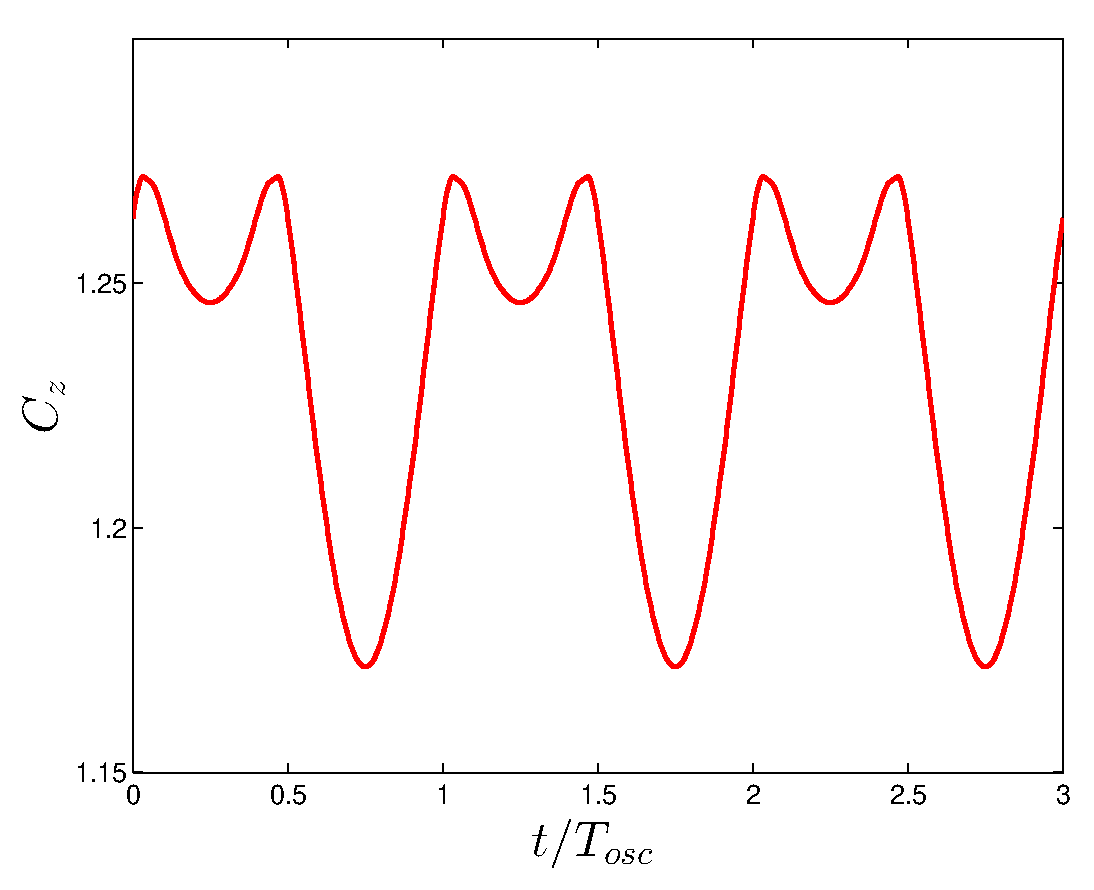
\includegraphics[width=1.0\columnwidth]{dynamic_nonlinear_cz_re1e6}
		\caption{Dynamic response $C_{z}(t)$}
		\label{fig:dynamic_nonlinear}
	\end{subfigure}
	\caption{Quasi-steady response of $C_{z}$ in the non-linear region ($1.7<\alpha<3.7$).}
	\label{fig:nonlinear_cz_response}
\end{figure}
While this may be a hypothetical case, it is reasonable to expect that for a small enough value of $k$, and in the absence of hysteresis there would be no perceptible dynamic effects and the flow would adjust to the slowly varying instantaneous angle of attack. As the value of $k$ is increased and unsteady effects become important, the dynamic response would slowly depart from this quasi-steady response. The simple example suggests that the classical linearized unsteady aerodynamic models, such as the one proposed by \cite{theodorsen35}, are no longer applicable even in the simplest quasi-steady conditions when inherent non-linearities exist in the static case. Unsteady aerodynamic models which account for this non-linearity of the static aerodynamic coefficients are necessary to accurately describe the unsteady response in such conditions.

\section{Stationary airfoil simulations}

\subsection{Parameter identification}

In order to study the dynamic response of unsteady natural laminar flow airfoils, it is necessary to establish the flow conditions for representative static angles of attack. However the high Reynolds numbers of the flow case make it prohibitively expensive to simulate several flow cases at different (static) angles of attack. To reduce the computational cost and narrow down the parameter range, we make use of experimental data provided by \cite{lokattthesis} and also perform calculations using XFOIL. Two factors govern the final choice of parameter selection for the unsteady simulations. 
\begin{itemize}
	\item Firstly, the earlier studies indicate that the dynamic non-linearities are observed when there is a free movement of transition on the suction side of the airfoil \citep{mai11,hebler13,lokattthesis}. Thus the parameter range must have large variations in transition location.  
	\item Secondly, in the previous section we established the link between the non-linearities in the temporal and static responses. Thus we also look for the $\alpha$ range that shows the strongest non-linearities in the static response of the lift coefficient.
\end{itemize}
\begin{figure}[h]
	\centering
	\begin{subfigure}[t]{0.48\textwidth}
		\caption{}		
		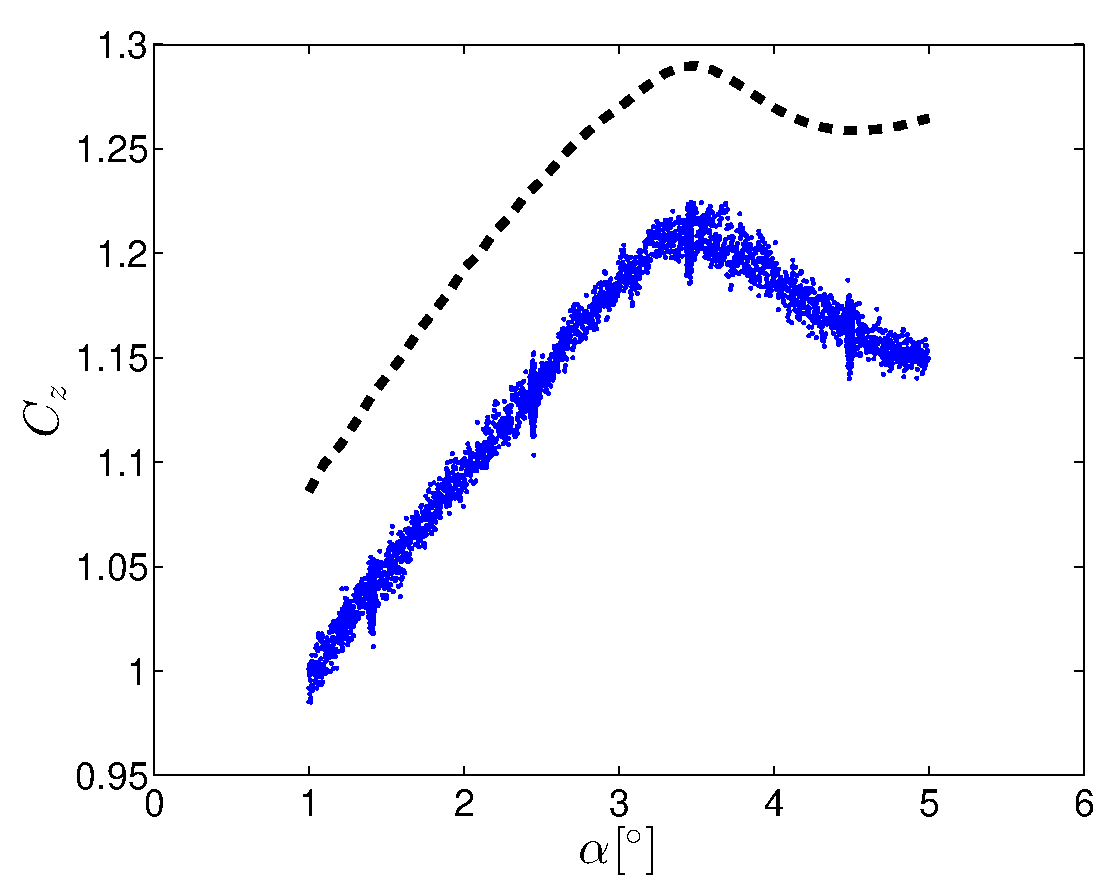
\includegraphics[width=1\textwidth]{765k_static_model_cz_xfoil}
		\label{fig:cz_static_xfoil}
	\end{subfigure}
	\begin{subfigure}[t]{0.48\textwidth}
		\caption{}		
		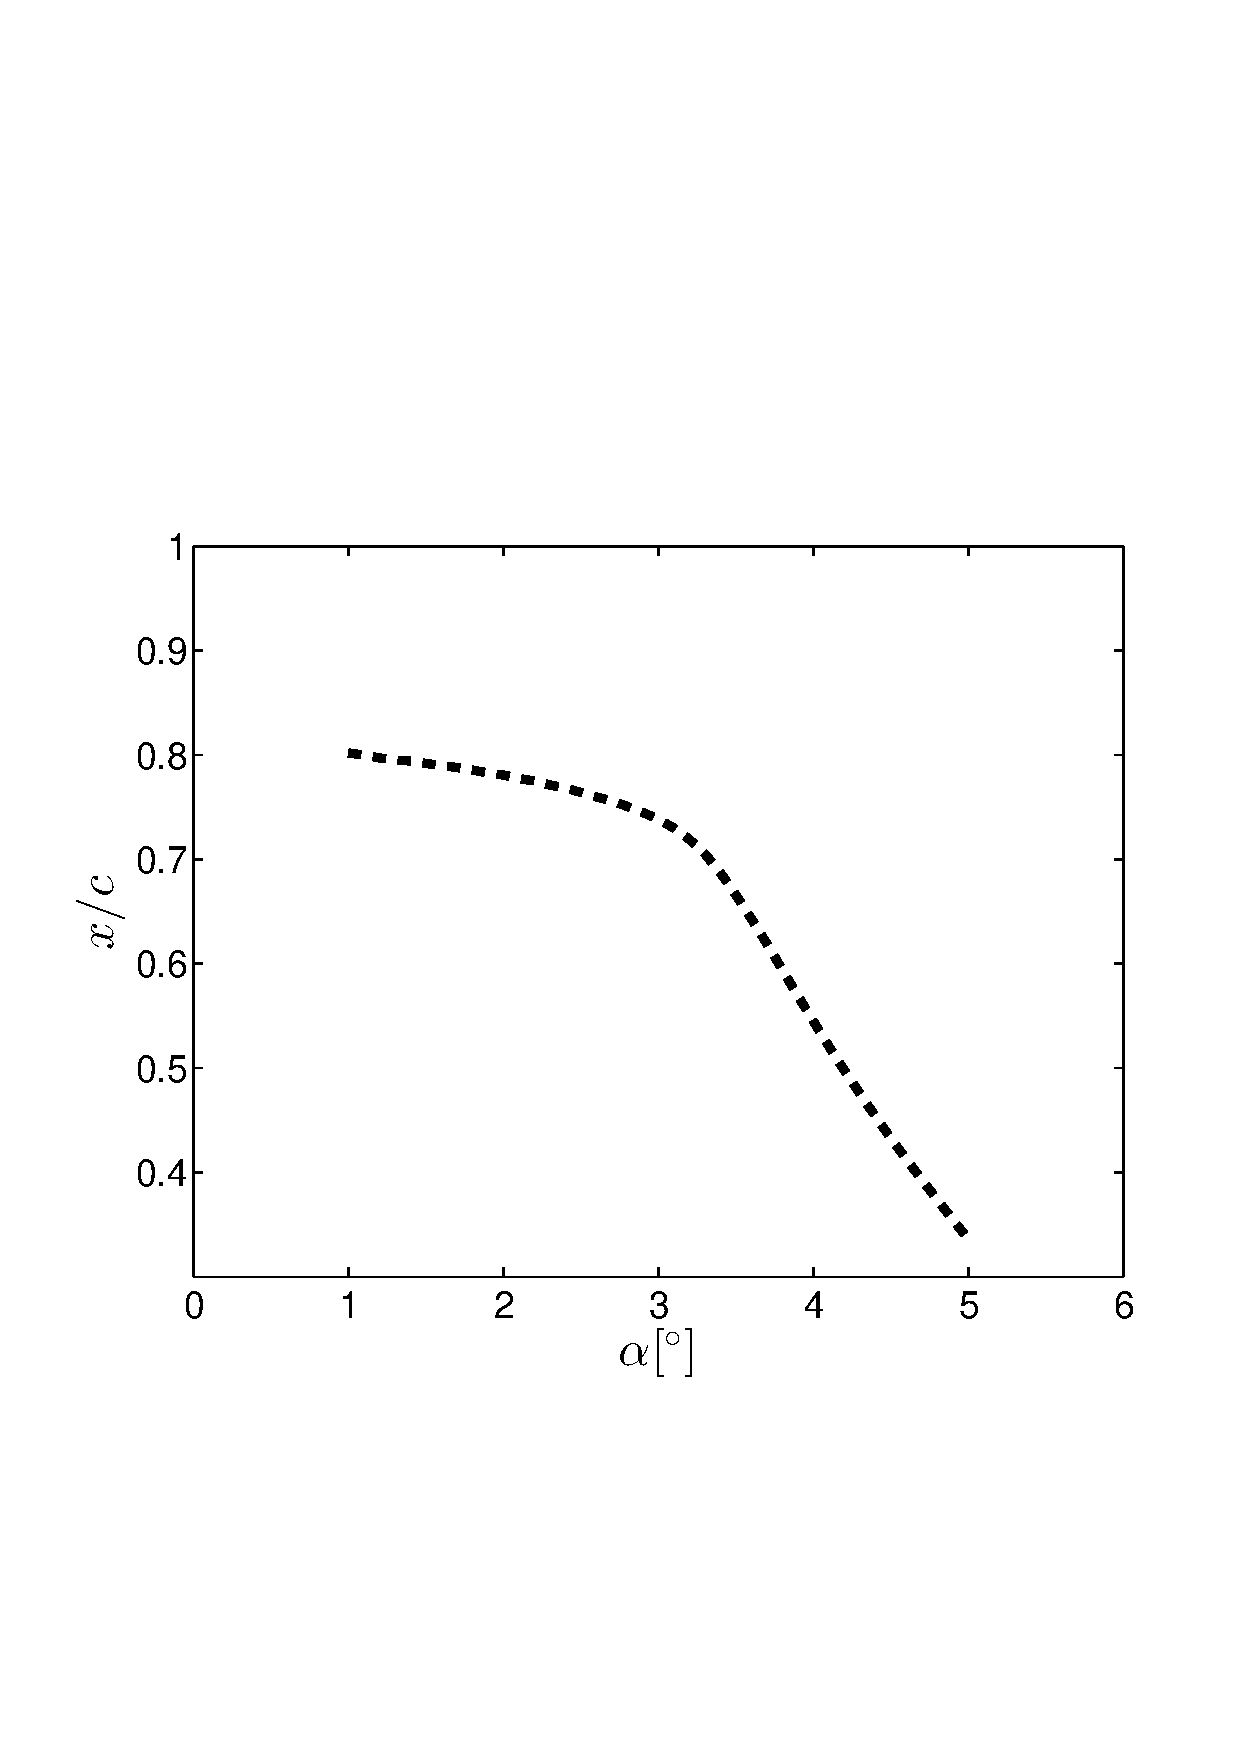
\includegraphics[width=1\textwidth]{765k_static_model_tr_xfoil}
		\label{fig:tr_static_xfoil}
	\end{subfigure}	
	\caption{Static aerodynamic characteristics of the NLF airfoil obtained from XFOIL calculations. Normal force coefficient (left) and transition location (right) variation with $\alpha$.}
	\label{fig:static_characteristics}
\end{figure}
The static response curves for the airfoil obtained using XFOIL as well the experimental data from \cite{lokattthesis} are shown in figure~\ref{fig:cz_static_xfoil}. While the experimental data and XFOIL calculations differ in magnitude, the range of angle of attack where qualitative changes take place is the same. In both cases the static response curve is linear between $1^{\circ}<\alpha<3^{\circ}$ and at around $\alpha=3.4^{\circ}$ the static curves strongly depart from their linear behavior, with the lift coefficient decreasing with increasing $\alpha$. Figure~\ref{fig:tr_static_xfoil} shows the variation of transition location on the suction side of the airfoil as predicted by XFOIL. Within the same range where non-linearities are observed in the static lift coefficient ($\alpha>3.4^{\circ}$), there is a sharp change in the slope of the transition location curve. Between $1^{\circ}<\alpha<3^{\circ}$ the transition location has a very slow upstream movement, while for $\alpha>3.4^{\circ}$, the upstream movement is much more rapid with respect to angle of attack. Both governing factors mentioned earlier indicate the same angle of attack region where non-linearities are to be expected (\textit{i.e} $\alpha\approx3.4^{\circ}$). Thus the pitching range where non-linearities are expected to show up strongly is near $\alpha\approx3.4^{\circ}$. Therefore this is defined as the mean angle of attack of oscillation. The pitch amplitude is taken to be small in accordance with the experimental results of \cite{lokattthesis}. The pitching motion of the unsteady case may be described by equation~\ref{eqn:unsteady_alpha}:
\begin{align}
	\alpha(t) = \alpha_{0} + \Delta\alpha\sin(\Omega (t-t_{0}) + \phi_{0}).
	\label{eqn:unsteady_alpha}
\end{align}
where $\alpha_{0}=3.4^{\circ}$ is the mean angle of attack, $\Delta\alpha=1.0^{\circ}$ is the pitch amplitude, $\Omega$ is the angular frequency of oscillation, $t$ represents the simulation time, $t_{0}$ is the starting time of the pitching motion and $\phi_{0}$ is the initial phase at the start of the oscillations.

In order to verify the static characteristics observed in experiments and also predicted by XFOIL, simulations of stationary airfoils are performed in the range chosen above to ensure that the expected variation of transition location is captured by the numerical simulations. 

\subsection{Computational Setup}

The numerical simulations are set up to perform wall-resolved large-eddy simulations (LESs) of the stationary and pitching airfoils. All numerical simulations are carried out using Nek5000 \citep{nek5000}. The setup is done in a manner very similar to our previous works relating to simulations of flow around airfoils \citep{hosseini16,proc-tsfp10-vinuesa,proc-tsfp10-negi}. The spectral-element mesh is generated using \textit{ANSYS}\textsuperscript{\textregistered} ICEMCFD, which is structured and orthogonal near the airfoil surface. The numerical simulation is set up such that the final resolution utilizes an $11^{th}$ order polynomial representation for the velocity and a staggered $9^{th}$ order representation for the pressure. The Navier--Stokes equations are solved using the Arbitrary-Lagrangian-Eulerian (ALE) framework \citep{ho90,ho91} to account for the motion of boundary and the internal points. The coordinate system is defined such that the $x$ direction is aligned with the inflow direction, $z$ is the spanwise homogeneous direction and $y$ is normal to the airfoil plane. All length scales are normalized by the chord length $c$, and velocities are normalized by the free-stream velocity, $U_{\infty}$. The far field boundaries are two chords away from the airfoil leading edge in either direction and the outflow boundary is four chords downstream from the airfoil leading edge. The inlet is designed as a curved inflow boundary with a constant radial distance of two chords from the leading edge of the airfoil. The spanwise width of the computational domain is $l_{z}=0.15c$. Periodic boundary conditions are imposed on the spanwise boundaries, while the energy-stabilized outflow condition \citep{dong2014} is imposed on the outflow boundary. A URANS simulation is performed using the transition $k$-$\Omega$ SST model \citep{langtry09} for the same case with far-field and outflow boundaries set at a 100 chords distance. Time-averaged velocity field data from the URANS simulation is extracted for the locations corresponding to the domain boundaries of the LES simulation. This extracted data is imposed as a Dirichlet boundary condition on the inlet and far-field boundaries. In order to simulate low turbulence flight conditions, free-stream turbulence of intensity $Ti=0.1\%$ is superimposed on the Dirichlet boundary conditions. The free-stream turbulence is generated using Fourier modes with a von K\'arm\'an spectrum. The integral length scale of the spectrum is set to $l=0.01$ which is approximately 5-10 times the boundary layer height near the leading edge. The procedure is similar to the one described in \cite{schlatterdiploma,brandt04,schlatter08}, where it has been used for the study of by-pass transition in flat-plate boundary layers. It has also been used for wind turbine simulations \citep{kleusberglicenciate} and in our earlier work on pitching airfoils at $Re_{c}=100,000$ \citep{proc-tsfp10-negi}.

The grid resolution on the airfoil surface varies with the chord-wise location in accordance with the changing boundary layer characteristics. Thus the guidelines for grid design use the following criteria:
\begin{itemize}
	\item[$\bullet$] For $0.1<x/c<0.6$, $\Delta x^{+}=18$, $\Delta y_{wall}^{+}=0.64$ and $\Delta y_{max}^{+}=11$, on the suction side and use the local wall-shear ($\tau_{w}$) values on the airfoil. Since the flow is expected to be laminar on the pressure side, the stream-wise resolution is slightly relaxed to $\Delta x^{+}=25$ while keeping the same wall-normal resolution.
	\item[$\bullet$] For $x/c<0.1$, the peak $\tau_{w}$ value over the suction side of the airfoil is used to estimate the grid spacing for both the suction and pressure sides.
	\item [$\bullet$] for $x/c>0.6$, the suction side experiences a large adverse pressure gradient which significantly reduces $\tau_{w}$ values. Therefore, the $\tau_{w}$ values from the pressure side are used for both the suction and pressure sides.
	\item [$\bullet$] A structured mesh is used, which is extruded in the span-wise direction. Hence the spanwise resolution is constant throughout the domain. The resolution is set to $\Delta z^{+}=12$, where the the peak $\tau_{w}$ value from the suction side is used.
\end{itemize}
The symbol $^{+}$ indicates normalization with inner units using kinematic viscosity $\nu$, and local friction velocity $u^{*}$. Wall-shear stress data is obtained using XFOIL to estimate the local friction velocity. A trip is introduced in XFOIL at $x/c\approx0.1$ to obtain turbulent wall-shear values on both the suction and pressure sides of the airfoil. A different criterion is needed for defining the resolution in the wake where the wall-based criteria are not valid. Accordingly, the URANS data is used to estimate the Kolmogorov length scale ($\eta$) in the wake region. The grid in the wake region is designed such that the average grid spacing in the near wake ($1<x/c<2$) follows the criteria: $\Delta x/\eta < 9$. For $x/c>2$ the grid spacing in the wake is slowly increased such that $\Delta x/\eta \approx 20$ near the outflow boundary at $x/c=4$.

Note that the above guidelines are for the final resolution of the numerical simulation. In our methodology we simulate the initial transients with a lower order polynomial representation on the same spectral-element grid and slowly increase the polynomial order. Currently, only the results from the low order polynomial simulations ($5^{th}$ order for the velocity) are reported. The effective grid spacings for the current results is therefore twice the values reported above. Nonetheless, tests with stationary airfoil simulations indicate that the qualitative features of the flow do not change with changing polynomial orders. 

\subsection{Stationary simulation results}

In accordance with the angle of attack range selected earlier, we perform two simulations with a stationary airfoil, with angles of attack corresponding to the two extremities of the pitching cycle, \textit{i.e.} at $\alpha=2.4^{\circ}$ and $\alpha=4.4^{\circ}$. Figure~\ref{fig:la2_750k_stationary} shows the instantaneous vortical structures identified by the $\lambda_{2}$ criterion \citep{jeong95}. From the figures it is clear that the transition occurs at widely different chord-wise locations for the two angles of attack, which is in accordance with the predictions of XFOIL as seen earlier in figure~\ref{fig:tr_static_xfoil}.
\begin{figure}[h]
	\centering
	\begin{subfigure}[t]{0.9\textwidth}
		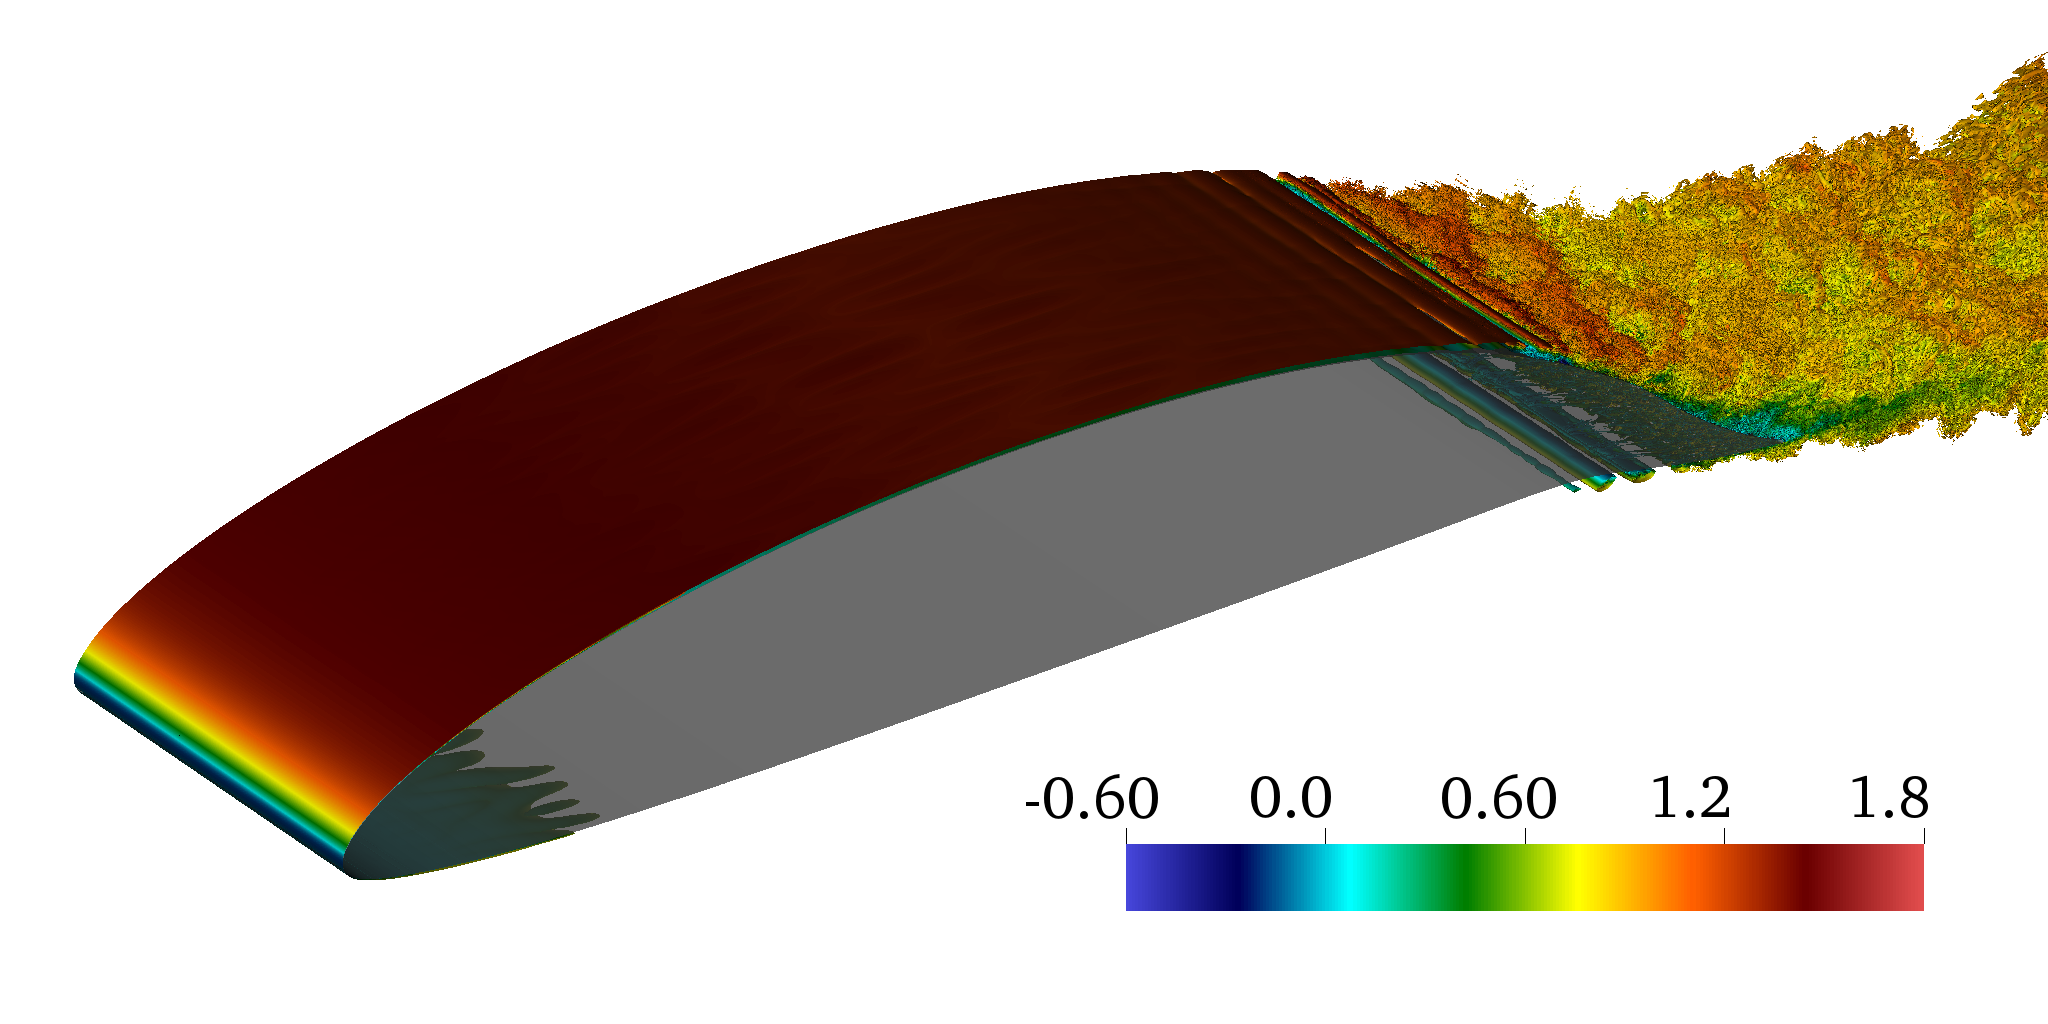
\includegraphics[width=1\textwidth]{pitch_re750k0001}
		\caption{$\alpha=2.4^{\circ}$}
		\label{fig:la2_aoa24}
	\end{subfigure}
	\begin{subfigure}[t]{0.9\textwidth}
		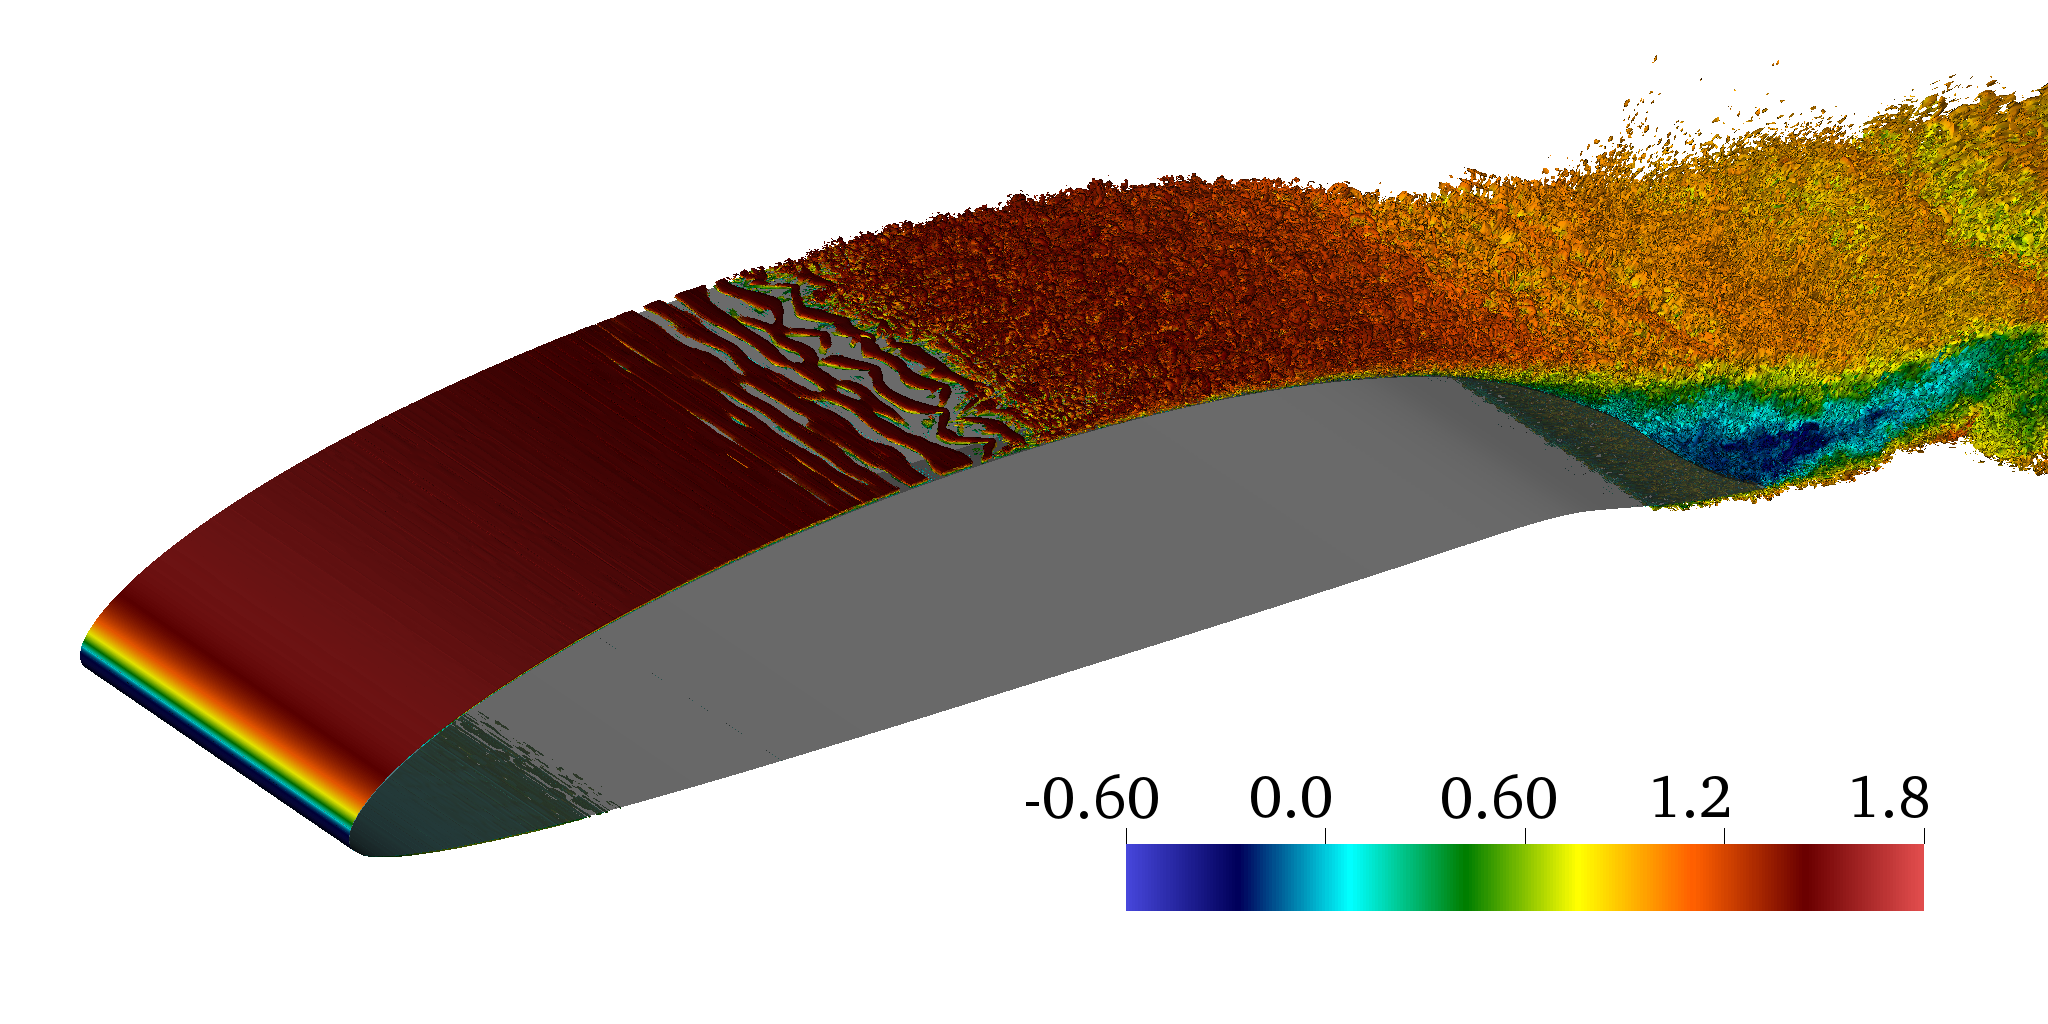
\includegraphics[width=1\textwidth]{pitch_re750k0002}
		\caption{$\alpha=4.4^{\circ}$}
		\label{fig:la2_aoa44}		
	\end{subfigure}	
	\caption{Instantaneous vortical structures identified by the $\lambda_{2}$ criterion for the two stationary angle of attack simulations.}
	\label{fig:la2_750k_stationary}
\end{figure}
The instantaneous structures for both cases are extracted after running the two simulations for about 6 flow through times. After the initial transients are convected away, the overall qualitative state of the flow does not change and the transition location remains constant. To ensure that the low order of the simulations is not affecting the transition location, and thus the overall qualitative flow state, the simulation with the lower angle of attack ($\alpha=2.4^{\circ}$) is restarted with a higher polynomial order ($N=8$) and the simulation is continued for about 1 flow over time. No qualitative change is detected in the flow state and the transition location does not change.

\section{Unsteady results}

\subsection{Lift coefficient}
Once the flow state for the stationary airfoil cases is established, oscillations of a pitching airfoil are performed with the pitching motion prescribed by equation~\ref{eqn:alpha_inst}. The angular frequency ($\Omega$) of the oscillation is chosen such that the non-dimensional reduced frequency, $k=0.4$ and the pitch axis is located at $(x_{0},y_{0})=(0.35,0.034)$. The time period of oscillation ($T_{osc}$) for the chosen reduced frequency is equal to $7.85$. The pitching simulations are started from the solutions of the stationary airfoil simulation at the angle of attack of $\alpha=2.4^{\circ}$. This point represents the minimum of the pitch cycle and starting the pitching motion from this minimum allows us to smoothly increase the angular velocity from zero. Thus no impulsive velocities are imparted to the airfoil when the pitching motion starts. The oscillatory motion is thus prescribed by equation~\ref{eqn:unsteady_alpha_2}:
\begin{subequations}
	\begin{align}
		\alpha(t) = \alpha_{0} + \Delta\alpha\sin(\Omega (t-t_{0}) + \phi_{0}), %\\
	%	\alpha_{0}=3.4^{\circ} & \Delta\alpha=1.0^{\circ} & t_{0}=6.0 & \beta=-\pi/2 \nonumber	
	\end{align}
	\begin{align}
		\text{with}\hspace{10pt}\alpha_{0}=3.4^{\circ}, \hspace{20pt} & \Delta\alpha=1.0^{\circ}, & t_{0}=6.0\hspace{10pt} \text{and} \hspace{10pt}& \phi_{0}=-\pi/2.
	%\label{eqn:unsteady_alpha_parameters}	
	\end{align}
\label{eqn:unsteady_alpha_2}
\end{subequations}
\begin{figure}[h]
	\centering
	\begin{subfigure}[t]{0.48\textwidth}
		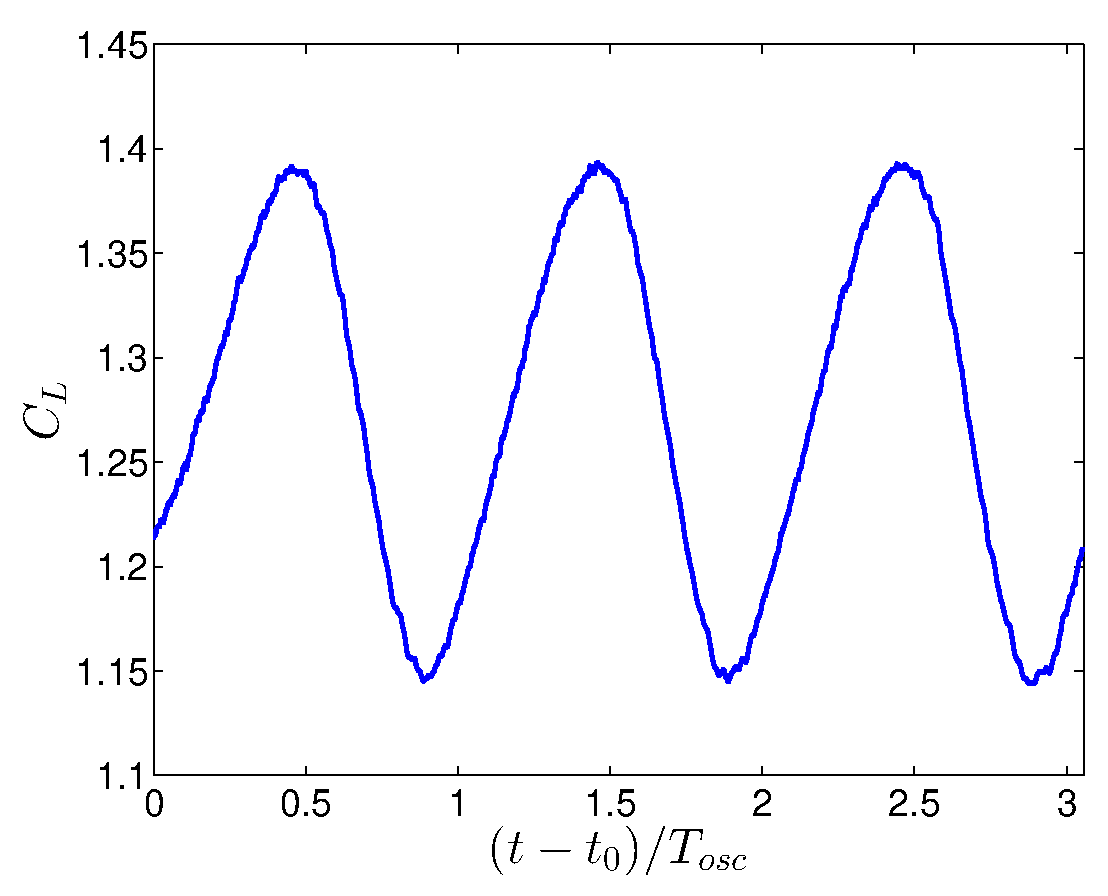
\includegraphics[width=1\textwidth]{cl-time-alpha750k}
		\caption{}
		\label{fig:750k_cl_time_alpha}		
	\end{subfigure}
	\begin{subfigure}[t]{0.495\textwidth}
		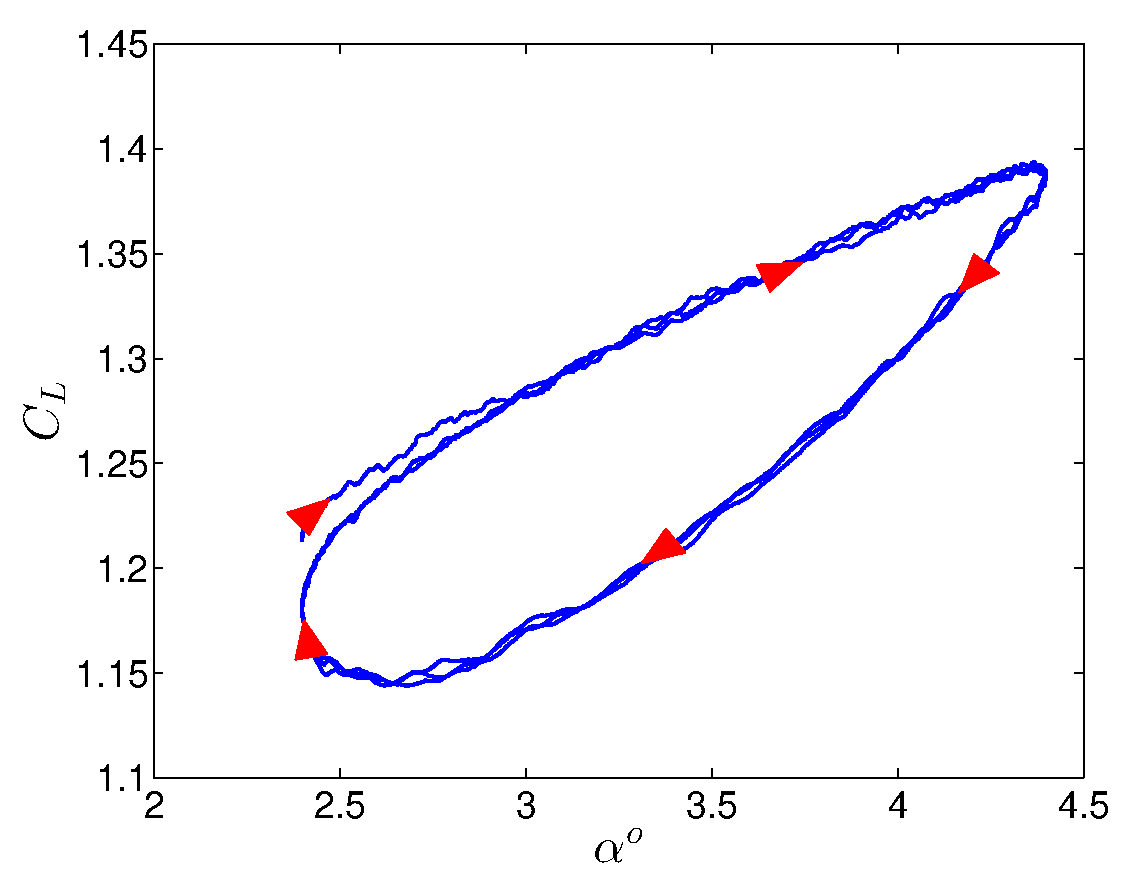
\includegraphics[width=1\textwidth]{cl-alpha750k}
		\caption{}
		\label{fig:750k_cl_alpha}			
	\end{subfigure}	
	\caption{Variation of unsteady lift coefficient with time (left) and instantaneous angle of attack (right). Red arrows in the phase portrait indicate direction of time.}
	\label{fig:750k_unsteady_lift}
\end{figure}

Figure~\ref{fig:750k_unsteady_lift} shows the variation of the unsteady lift coefficient $C_{L}$ with time, as well as the phase portrait with respect to $\alpha$. One can immediately observe from the phase portrait (figure~\ref{fig:750k_cl_alpha}) that (after a small initial transient) no large deviations of the lift coefficient occur between consecutive cycles of oscillation, indicating that the flow has settled into a regular cyclic state and further qualitative changes that may be transient in nature are not expected to occur with more pitch cycles. While the non-linearity is less obvious from the time series plot, the phase portrait clearly shows the non-linearities by way of a distorted ellipse. Linear responses trace an ellipse in the phase portrait with respect to angle of attack. Distortions of the ellipse indicate the presence of additional frequencies in the time response.

\subsection{Unsteady boundary layer}
The spatio-temporal variation of the boundary layer can be analyzed via the instantaneous wall-shear stress. Figure~\ref{fig:space-time_color750k} shows the space-time variation of the instantaneous, spanwise averaged wall-shear stress on the suction side of the airfoil surface. Areas which are strongly red in color are high shear-stress regions and thus signify turbulent flow (except the region very close to the leading edge which has a very thin boundary layer). The turbulent regions show periodic bumps in the space-time plot which are indicative of the movement of transition throughout the oscillation phases. This is consistent with the earlier studies of \cite{mai11,hebler13} and \cite{lokattthesis} which suggest the free movement of transition is responsible for non-linearities in the aerodynamic force coefficients. Figure~\ref{fig:750k_cf_x} shows horizontal slices from the space-time plot for two different time instants which represent the instantaneous spatial variations of $\tau_{w}$.  
\begin{figure}[!h]
   	\centering
	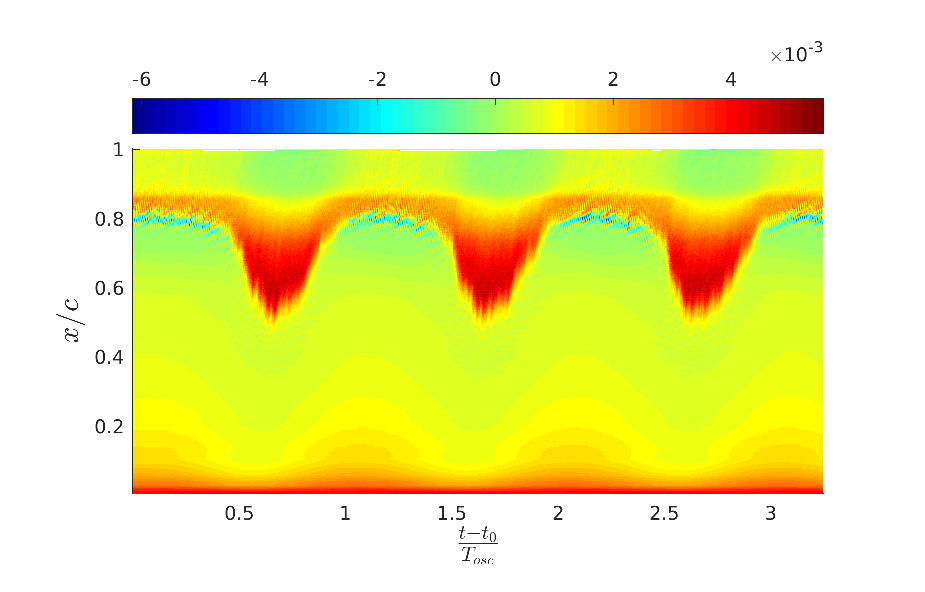
\includegraphics[width=\textwidth]{cf_time_surf750k}		
	\caption{Spatio-temporal variation of wall-shear stress. The $y$-axis represents the chord-wise location while the $x$-axis represents the normalized simulation time. The colors represent the instantaneous, spanwise-averaged wall-shear stress value, $\tau_{w}(x,t)$, for each chord-wise location.}	
	\label{fig:space-time_color750k}
\end{figure}
\begin{figure}[!h]
	\centering
	\begin{subfigure}[t]{0.49\linewidth}
		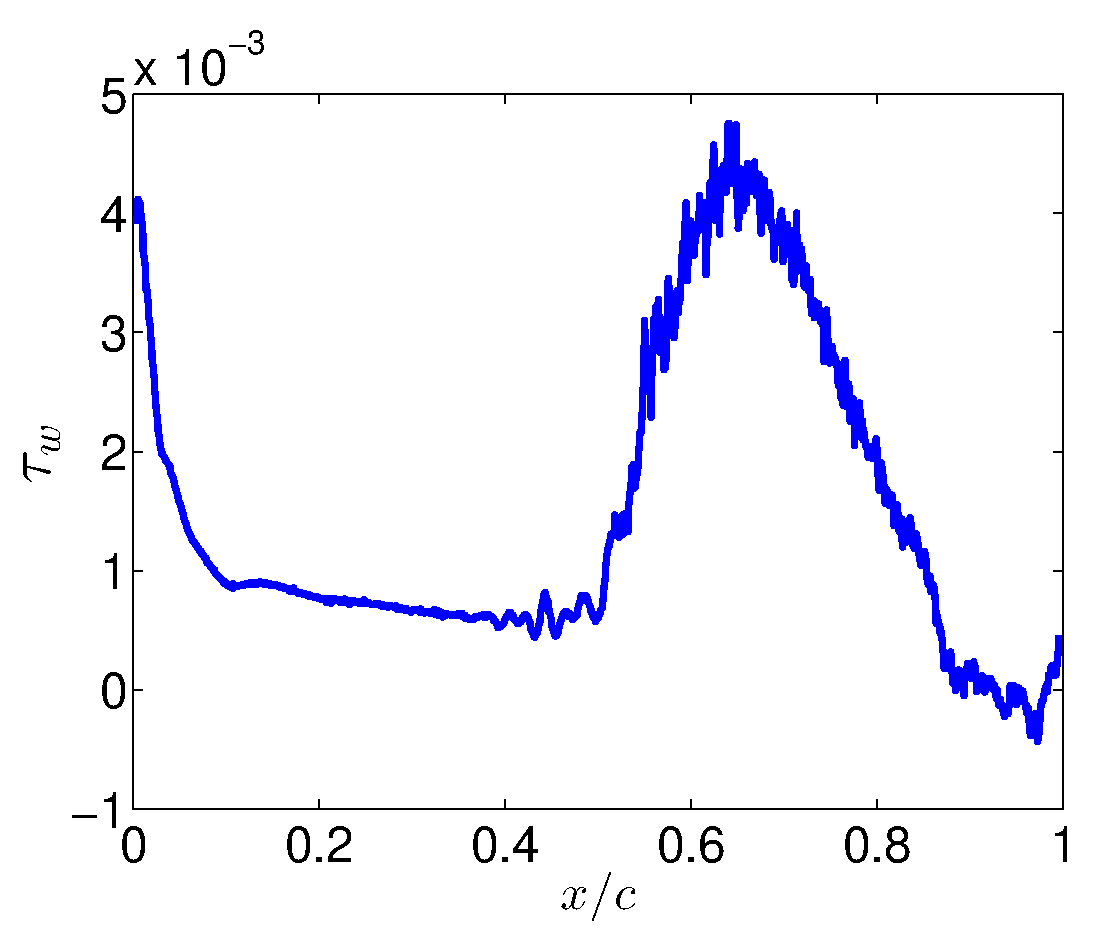
\includegraphics[width=\linewidth]{pitch750k_t01_60}
%		\label{fig:750k_cf_x_t1.60}
	\end{subfigure}
	\begin{subfigure}[t]{0.49\textwidth}			
		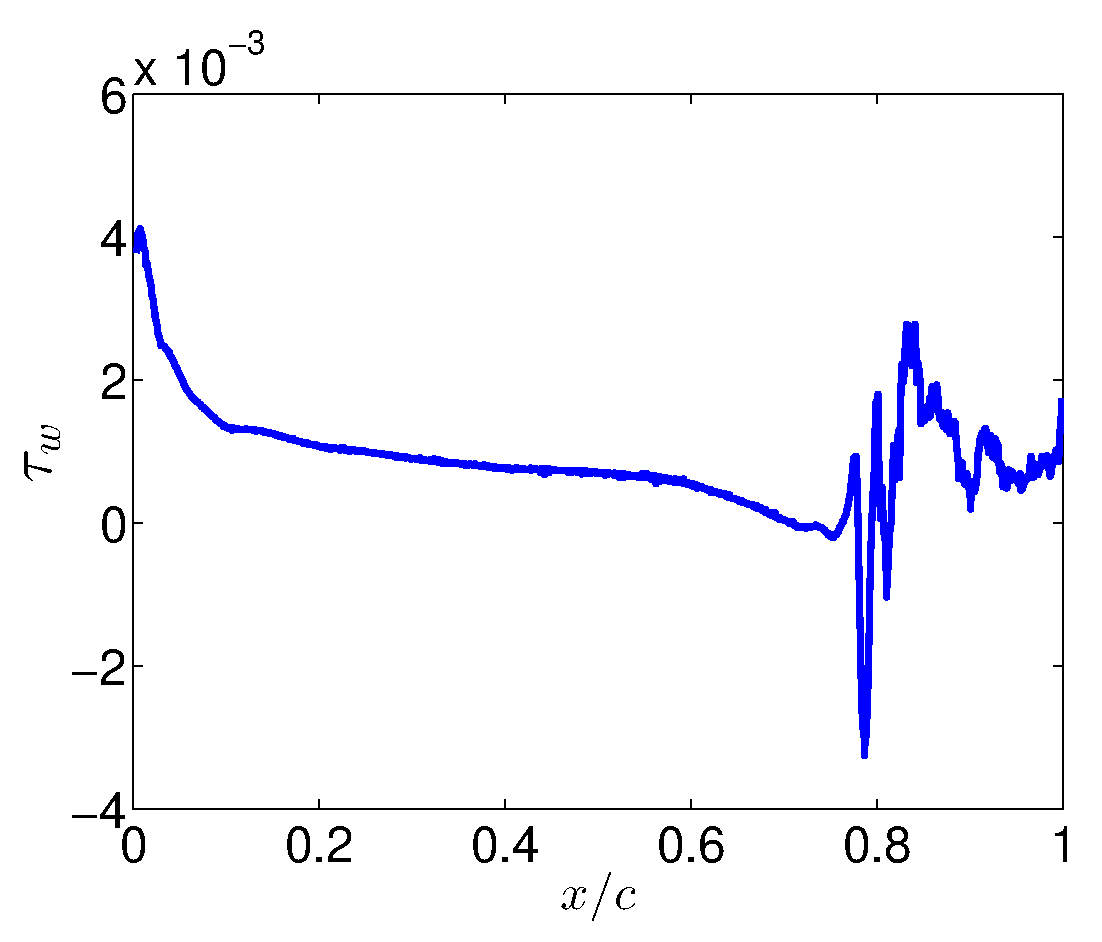
\includegraphics[width=\linewidth]{pitch750k_t02_25}
%		\label{fig:750k_cf_x_t2.25}
	\end{subfigure}
	\caption{Instantaneous chord-wise variation of $\tau_{w}(x,t)$. Figures represent time-instants when the transition is close to its most upstream location at time $(t-t_{0})/T_{osc}=1.60$ (left) and when it is close to the most downstream location at time $(t-t_{0})/T_{osc}=2.25$ (right).}
	\label{fig:750k_cf_x}	
\end{figure}

%\begin{figure}[h]
%   	\centering
%   	\begin{minipage}{0.55\linewidth}
%   		\begin{subfigure}[t]{\linewidth}
%   			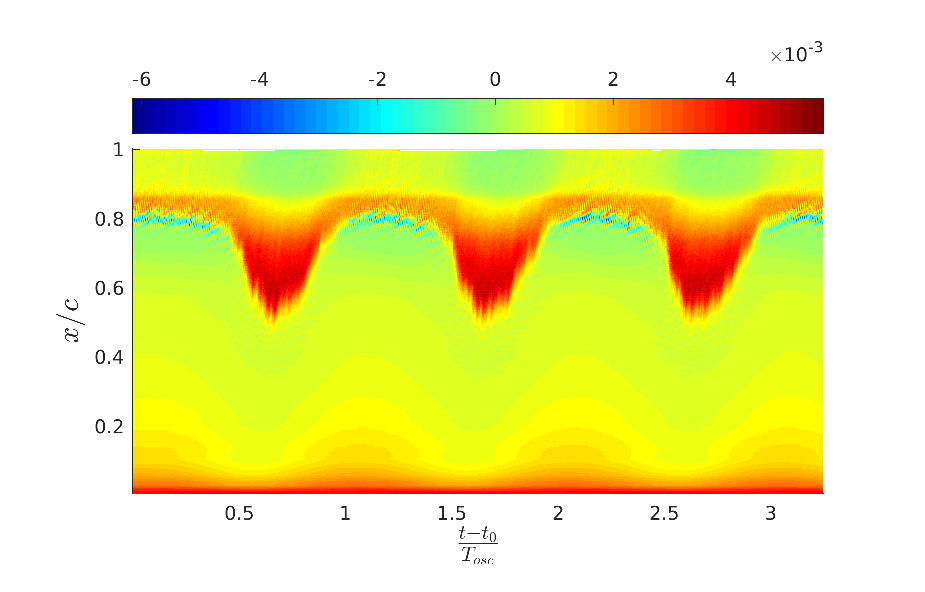
\includegraphics[width=\linewidth]{cf_time_surf750k}
%   			\caption{Spatio-temporal evolution of $\tau_{w}$}
%   			\label{fig:space-time_color750k}
%   		\end{subfigure}
%   	\end{minipage}   	
%   	\begin{minipage}{0.44\linewidth}
%   		\begin{subfigure}[t]{\linewidth}
%   			\caption{}   			
%   			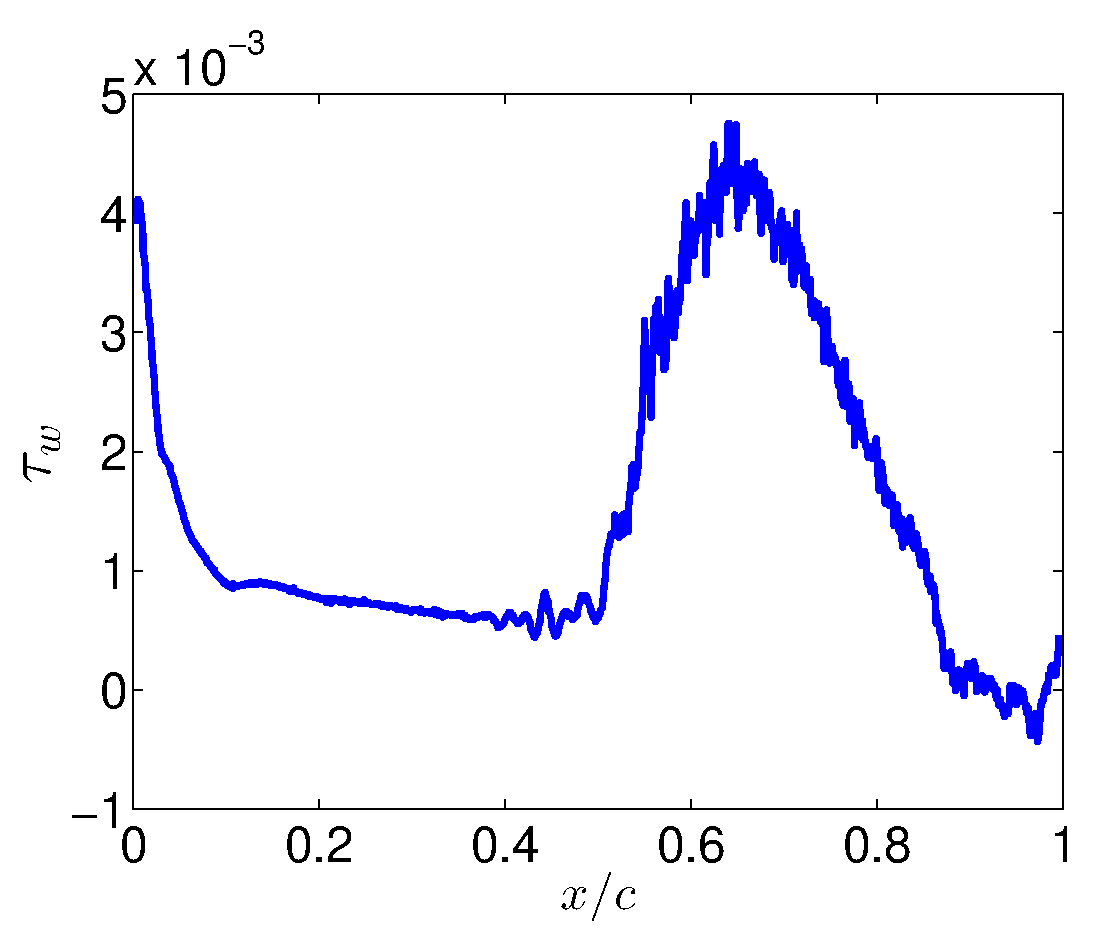
\includegraphics[width=\linewidth]{pitch750k_t01_60}
%   			\label{fig:750k_cf_x_t1.60}
%   		\end{subfigure}
%   		\begin{subfigure}[t]{\textwidth}
%   			\caption{}   			
%   			\includegraphics[width=\linewidth]{pitch750k_t02_25}
%   			\label{fig:750k_cf_x_t2.25}
%   		\end{subfigure}
%   	\end{minipage}
%   	\hfil
%   	\caption{The color plot on the left (a) shows the space-time variation of wall-shear stress. The $x$-axis represents the chord-wise location while the $y$-axis represents the normalized simulation time. The colors represent the instantaneous, spanwise averaged wall-shear stress value, $\tau_{w}(x,t)$, for each chord-wise location. Figures on the right show the chord-wise variation of $\tau_{w}(x,t)$ at two different time instances when the transition is close to its most upstream location at time $(t-t_{0})/T_{osc}=1.60$ (b) and when it is close to the most downstream location at time $(t-t_{0})/T_{osc}=2.25$ (c).}
%   	\label{fig:space-time_cf750k}
%\end{figure}

\subsection{Transition location}
For further analysis a quantification of the transition point variation is necessary and to this end the instantaneous transition point needs to be defined. Since the transition changes continuously with time, a criterion is required which is based on the instantaneous state of the flow rather than the long-time statistical average. In order to define quantities representative of the instantaneous state of the flow, we take advantage of the homogeneous direction and and also perform a temporal averaging operation for a very short duration in time. Thus we evaluate statistical quantities ``$\overline{q}(x,y,t)$'' which are defined as in equation~\ref{eqn:750k_inst_q}:
\begin{align}
	\overline{q}(x,y,t) = \left(\frac{1}{z_{max}-z_{min}}\right)\left(\frac{1}{\Delta t}\right)\int_{t'=t}^{t'=t+\Delta t}\int_{z=z_{min}}^{z=z_{max}}q(x,y,z,t')\ dz\ dt'.
	\label{eqn:750k_inst_q}
\end{align}
Here $(z_{max} - z_{min})$ is the spanwise width of the computational domain and $\Delta t$ is a short temporal averaging period. In order for such a quantity to be representative of the instantaneous state of the flow, the time duration of the averaging must be small. For the current case we use $\Delta t=3\times10^{-2}$, which amounts to $0.38\%$ of the oscillation time period during which the flow can be assumed to remain approximately in the same state. Using this procedure we evaluate the fluctuating Reynolds stress, $\overline{u'v'}(x,y,t)$. Large Reynolds stresses indicate turbulent flow, thus the most upstream location (on the suction side) where the the quantity $\overline{u'v'}(x,y,t)$ becomes large is denoted as the transition location. In order to prescribe a suitable threshold for ``large", the maximum value of $|\overline{u'v'}(x,y,t)|$ across the entire boundary layer is evaluated for all times. This maximum value does not have very large variations, staying within the same order of magnitude with its mean value being $|\overline{u'v'}|_{max}=10^{-2}$. The threshold for determining transition is set to $5\%$ of this value. The transition point is thus the first point where $|\overline{u'v'}(x,y,t)|>5\times10^{-4}$. Since the criterion is a bit arbitrary, it is cross-checked by evaluating the variance of the spanwise velocity fluctuations $\overline{w'w'}(x,y,t)$ following the same procedure. In this case the threshold is set as $|\overline{w'w'}(x,y,t)|>10^{-3}$, since the peak spanwise fluctuation intensity is found to be nearly twice the peak Reynolds stress. Growing spanwise velocity fluctuations indicate the onset of three-dimensionality, and thus they constitute a physically meaningful indicator of transition. Despite the rather ad-hoc nature of the threshold criteria, the qualitative picture of transition movement is not very sensitive to small changes in the threshold. Reducing or increasing the thresholds by a factor of 2 still produces the same qualitative trends (not shown). Figure~\ref{fig:750k_tr_alpha} shows the phase portrait of the transition location, determined by the aforementioned criteria. The two criteria show a good quantitative agreement with each other. Figure~\ref{fig:750k_space-time_tr} shows the calculated transition location (using $\overline{u'v'}$) superposed on the wall-shear stress space-time plot. The calculated transition locations are consistent with the picture of wall-shear stress with transition marginally preceding regions of turbulent flow.

%\begin{figure}[43]{r}{0.58\textwidth}
%	\centering	
%	\includegraphics[width=0.50\textwidth]{750k_transition_alpha}
%	\caption{Empirically determined transition location using the $|\overline{u'v'}|$ and $|\overline{w'w'}|$ criteria. Arrows indicate the forward direction in time.}
%	\label{fig:750k_tr_alpha}
%	\includegraphics[width=0.55\textwidth]{cf_time_surf750k_tr}
%	\caption{Empirically determined transition location (magenta curve) overlay-ed on the space-time plot of $\tau_{w}$.}
%	\label{fig:750k_space-time_tr}
%\end{figure}

\begin{figure}[h]
	\centering	
	\includegraphics[width=0.60\textwidth]{750k_transition_alpha}
	\caption{Empirically determined transition location using the $|\overline{u'v'}|$ and $|\overline{w'w'}|$ criteria. Arrows indicate the forward direction in time.}
	\label{fig:750k_tr_alpha}
\end{figure}
\begin{figure}
	\includegraphics[width=\textwidth]{cf_time_surf750k_tr}
	\caption{Empirically determined transition location (magenta curve) superposed on the space-time plot of $\tau_{w}$.}
	\label{fig:750k_space-time_tr}
\end{figure}

The phase portrait in figure~\ref{fig:750k_tr_alpha} clearly shows the asymmetric flow states between the pitch-up (upper branch) and the pitch-down (lower branch) phases of the oscillation. During the pitch-up phase the transition point is near the trailing edge and has a very slow upstream movement for most part of pitch-up cycle, and later moves upstream sharply at the end of the pitch-up phase. During the pitch-down phase of the oscillation, the transition location is constantly moving downstream with the motion appearing much more gradual in phase space. This phase portrait can be transformed to give a more insightful picture of the ongoing dynamics by using a phase-lag concept. In this transformation we consider the evolution of the boundary layer with respect to an effective angle of attack $\alpha_{e}$ which differs from the instantaneous angle of attack by a phase-lag. The physical interpretation of the phase-lag is a simple one, \textit{i.e.} the boundary layer adjusts to the changing flow-field in a quasi-steady manner, however there is a time lag between the airfoil motion and the boundary-layer adjustment, and the effective angle of attack that the boundary layer perceives is different from the instantaneous angle of attack. The expression for the effective angle of attack for the current case may be written by adding an additional term to equation~\ref{eqn:unsteady_alpha_2}
\begin{align}
	\alpha_{e}(t) = \alpha_{0} + \Delta\alpha\sin(\Omega (t-t_{0}) + \phi_{0} + \boldsymbol{\phi_{lag}}),
	\label{eqn:unsteady_alpha_3}
\end{align}
where $\boldsymbol{\phi_{lag}}$ is the phase lag between the instantaneous and effective angles of attack.
%\begin{wrapfigure}[22]{R}{0.58\textwidth}
%	\centering
%	\includegraphics[width=0.56\textwidth]{750k_transition_alpha_e}
%	\caption{Phase portrait of the transition location with respect the effective angle of attack($\alpha_{e}$). The blue lines represent the evaluated transition location (using $|\overline{u'v'}|$) and the black dashed line represents static transition location values obtained from Xfoil.}
%	\label{fig:750k_transition_phase_lag}
%\end{wrapfigure}

\begin{figure}[h]
	\centering
	\includegraphics[width=0.60\textwidth]{750k_transition_alpha_e}
	\vspace{5pt}
	\caption{Phase portrait of the transition location with respect to the effective angle of attack($\alpha_{e}$). The blue lines represent the evaluated transition location (using $|\overline{u'v'}|$) and the black dashed line represents static transition location values obtained from Xfoil.}
	\label{fig:750k_transition_phase_lag}
\end{figure}

The phase-lag concept is often used in unsteady aerodynamics \citep{theodorsen35,leishman00,bisplingoff00,mccroskey82,ericsson_stall88a} to describe the unsteady response of aerodynamic forces. In this case we apply the concept specifically to the evolution of the boundary layer. Figure~\ref{fig:750k_transition_phase_lag} shows the phase portrait with respect to the effective angle of attack, when evaluated using a phase lag of $\phi_{lag}=-1.0976$. What was initially a closed orbit in the $x/c-\alpha$ plane (figure~\ref{fig:750k_tr_alpha}) transforms into a single line when visualized in the $x/c-\alpha_{e}$ plane. Surprisingly, this new phase portrait corresponds well with the static transition curve calculated using XFOIL. While such a collapse seems remarkable at first, it simply implies a quasi-steady evolution of the boundary layer in time. The transition location can be considered as a scalar value which describes the instantaneous state of the boundary layer on the airfoil. If a boundary layer evolves in a quasi-steady manner in time, its trajectory in the $x/c-\alpha$ phase space would simply follow the trajectory of the static curve. For the unsteady cases one simply needs to consider the effective angle of attack perceived by the boundary layer, since the boundary-layer response lags behind the instantaneous angle of attack variations.
\section{An empirical unsteady model}
Given the failure of classical unsteady models to predict non-linear unsteady response, we build an empirical model which has its roots in the unsteady aerodynamic model of \cite{theodorsen35}, while utilizing the insight gained in the previous section on the quasi-steady evolution of the boundary layer over the airfoil. The model proposed by \cite{theodorsen35} incorporates several different forms of unsteady motions (pitching, plunging and flap rotations). Once simplified to pure pitch oscillations the model for the normal force coefficient reads as
\begin{align}
	C_{z}(t) = \underbrace{\pi [\dot{\alpha} - a\ddot{\alpha}]}_{\text{I}} + \underbrace{2\pi [\alpha + \dot{\alpha}(\frac{1}{2} - a)]}_{\text{II}}C(k),
\end{align}
where term I represents the added mass contribution to the normal force coefficient and term II may be viewed as the quasi-steady lift modulated by the Theodorsen transfer function $C(k)$. This modulation term represents the attenuation of the unsteady lift force due to the oscillating shed wake vorticity, and is a function of the reduced frequency only. Here $``a"$ is the distance of the axis of rotation from the mid chord location. The added-mass term is a purely harmonic term which represents the additional force on the airfoil due to the mass of the fluid close to the airfoil being accelerated along with the surface as the airfoil undergoes a pitching motion. Term II represents the effects of the quasi-steady lift force and may be reformulated as
\begin{align}
	2\pi [\alpha + \dot{\alpha}(\frac{1}{2} - a)] = 2\pi\alpha_{eff} = C^{inv}_{z}(\alpha_{eff}),
\end{align}
where $\alpha_{eff}$ is an effective angle of attack perceived by the boundary layer, which differs from the instantaneous angle of attack $\alpha$. Since the Theodorsen model is derived from inviscid assumptions of thin airfoil theory, the term $2\pi\alpha_{eff}$ is simply the normal force coefficient as predicted by the quasi-steady thin airfoil theory at an angle of attack of $\alpha_{eff}$, denoted here as $C_{z}^{inv}(\alpha_{eff})$. When non-linearities are present in the static $C_{z}$ curve, this assumption is clearly violated. Calculating the contribution of the quasi-steady term from the inviscid assumptions would lead to erroneous results. In order to account for these non-linearities, we make a similar quasi-steady assumption, wherein, we assume that to a first order approximation, the boundary layer evolves in a quasi-steady manner throughout the pitch cycle. The results of the previous section strengthen the validity of this assumption. However the effective angle of attack is different from the instantaneous angle of attack and the phase-lag is not known a-priori. Since the flow does not satisfy inviscid assumptions, the value of the quasi-steady term would need to be determined by an empirically calculated $C_{z}$ curve. Therefore we replace $C^{inv}_{z}(\alpha_{eff})$ with an empirically calculated static normal force coefficient curve, denoted as $C^{emp}_{z}(\alpha_{eff})$. The empirically calculated curve for a Reynolds number of $Re_{c}=10^{6}$ with the current airfoil is shown in figure~\ref{fig:cz_static}. Since it is unclear that the phase lag (or gain) for both the added mass term as well as the quasi-steady term would remain the same as when the inviscid thin airfoil theory applies, we leave these terms as parameters to be determined from the data. The empirical model thus reads
\begin{subequations}
	\begin{align}
		\label{eqn:phase_lag_cz}
		C_{z}(t) = A_{1}sin(\omega t + \theta) + C^{emp}_{z}(\gamma(t)),
	\end{align}
	\begin{align}
		\label{eqn:effective_alpha}	
		\gamma(t) = \alpha_{0} + \Delta\alpha sin(\omega t - \phi_{lag}).
	\end{align}
		\label{eqn:phase_lag_model}	
\end{subequations}
Where the instantaneous angle of attack follows the relation
\begin{align}
	\alpha(t) = \alpha_{0} + \Delta\alpha sin(\omega t).
\end{align}
Thus the empirical model has three independent parameters to be determined. $A_{1}$, which represents the strength of the added-mass term. $\theta$, which represents the phase gain/lag of this added-mass contribution with respect to the instantaneous angle of attack, and $\phi_{lag}$, which represents the phase-lag of the quasi-steady term. If the empirical $C^{emp}_{z}(\alpha)$ curve is linear with respect to $\alpha$, the time-response of the model will be purely harmonic.

The model parameters are then obtained using a least-squares fit to the experimental (or numerical) data. In the present work we utilize the unsteady experimental measurements of \cite{lokattthesis} to test the applicability of the model described by equation~\ref{eqn:phase_lag_model}. The measurements were carried out for a Reynolds number of $Re_{c}=10^{6}$ and $Re_{c}=7.5\times10^{5}$ for a wide range of angles of attack and with small amplitude pitch oscillations. The static $C_{z}$ curve required by the model was also obtained from the experimental data provided by \cite{lokattthesis}. Figure~\ref{fig:cz_static_exp} shows the static curve obtained in the experimental results for $Re_{c}=10^{6}$.
\begin{figure}[h]
	\centering
	\includegraphics[width=0.5\textwidth]{950k_static_model_cz}
	\vspace{5pt}
	\caption{The experimental static normal force coefficient curve $C_{z}^{emp}(\alpha)$ obtained by \cite{lokattthesis}.}
	\label{fig:cz_static_exp}
\end{figure}
Surprisingly, the simple model showed a good fit with the experimental data. Figure~\ref{fig:model_fits1} shows the least-squares fit for the data obtained at a mean angle of attack of $\alpha_{0}=2.8^{\circ}$, pitch amplitude of $\Delta\alpha=1^{\circ}$ and different reduced frequencies. The red dots indicate the experimental values while the solid black line is the least-squares fit to the experimental data. As can be seen in figure~\ref{fig:cz_static_exp}, the mean angle of $2.8^{\circ}$ places the oscillation region at the start of the $\alpha$ region exhibiting non-linearities in the static curve.
\begin{figure}[h]
	\centering
	\begin{subfigure}[b]{0.45\textwidth}
		\centering
		\includegraphics[width=1.0\columnwidth]{950k_time_plot_33_1}
		\caption{$k=0.01$}
		\label{fig:k_01}
	\end{subfigure}
	\begin{subfigure}[b]{0.45\textwidth}
		\centering
		\includegraphics[width=1.0\columnwidth]{950k_time_plot_33_3}
		\caption{$k=0.05$}
		\label{fig:k_05}
	\end{subfigure}
	\begin{subfigure}[b]{0.45\textwidth}
		\centering
		\includegraphics[width=1.0\columnwidth]{950k_time_plot_33_5}
		\caption{$k=0.10$}
		\label{fig:k_1}
	\end{subfigure}
	\begin{subfigure}[b]{0.45\textwidth}
		\centering
		\includegraphics[width=1.0\columnwidth]{950k_time_plot_33_9}
		\caption{$k=0.2$}
		\label{fig:k_2}
	\end{subfigure}	
	\caption{Least-squares fit of the empirical model to the experimental data for a mean angle of attack of $\alpha_{0}=2.8^{\circ}$, $\Delta\alpha=1^{\circ}$ and a selection of reduced frequencies $k$.}
	\label{fig:model_fits1}
\end{figure}
The good agreement is not confined to a single mean angle of attack. The model was tested with several different parameter combinations of mean angle of attack and reduced frequencies and a fairly good agreement was found for all cases considered, even for some cases with relatively high reduced frequencies of $k\approx0.4$. Figure~\ref{fig:model_fits2} shows another set of experimental data within the non-linear regime along with the least squares fit of the model.
\begin{figure}[h]
	\centering
	\begin{subfigure}[b]{0.45\textwidth}
		\centering
		\includegraphics[width=1.0\columnwidth]{950k_time_plot_35_1}
		\caption{$k=0.01$}
		\label{fig:k_01_2}
	\end{subfigure}
	\begin{subfigure}[b]{0.45\textwidth}
		\centering
		\includegraphics[width=1.0\columnwidth]{950k_time_plot_35_2}
		\caption{$k=0.025$}
		\label{fig:k_025_2}
	\end{subfigure}
	\begin{subfigure}[b]{0.45\textwidth}
		\centering
		\includegraphics[width=1.0\columnwidth]{950k_time_plot_35_8}
		\caption{$k=0.18$}
		\label{fig:k_18_2}
	\end{subfigure}
	\begin{subfigure}[b]{0.45\textwidth}
		\centering
		\includegraphics[width=1.0\columnwidth]{950k_time_plot_35_11}
		\caption{$k=0.26$}
		\label{fig:k_2_2}
	\end{subfigure}	
	\caption{Least-squares fit of the empirical model to the experimental data for a mean angle of attack of $\alpha_{0}=3.2^{\circ}$, $\Delta\alpha=1^{\circ}$ and different reduced frequencies $k$.}
	\label{fig:model_fits2}
\end{figure}
Thus the quasi-steady phase-lag concept for the temporal evolution of the boundary layer over the airfoil appears to be applicable for several different parameter values, even when boundary-layer transition location changes significantly. The model however is not predictive, but rather allows for a-posteriori analysis of the data since the phase lag/gain of the boundary-layer and added-mass terms are not known a-priori. It must be kept in mind however that only data from small-amplitude pitch oscillations with a relatively narrow range of reduced frequencies $k<0.4$ was available and thus the applicability of such a simple model for more general cases of pitching remains unknown. More data would be required to infer definitive trends of the model parameters ($A_{1},\theta,\phi_{lag}$) and to make conclusive remarks on the predictive capabilities of such a simple model.

%\FloatBarrier
\section{Conclusion and summary}
This report presents some of the initial results of LES of an unsteady natural laminar flow airfoil. The parameter range of the unsteady simulations was based on XFOIL calculations and experimental data. Preliminary simulations of stationary airfoils were performed to ensure the desired aerodynamic characteristics are captured by the numerical simulations. The unsteady simulations showed a non-linear response for the aerodynamic force coefficients while the unsteady boundary-layer development showed large variations of the point of transition over the suction side of the airfoil. These large variations in transition are shown to be linked to the static characteristics of the airfoil. The temporal variation can be related to the static transition curve with the use of a simple phase-lag concept, which implies that the boundary-layer evolution can be considered to be quasi-steady in time (at least as a first order assumption).

Based on this phase-lag and quasi-steady concept, an empirical model is developed to explain the non-linearities observed in the unsteady response of natural laminar flow airfoils. The empirical model has its roots in the unsteady model proposed by \cite{theodorsen35} and is able to model the aerodynamic non-linearities observed in the experiments of \cite{lokattthesis}.

Higher resolution simulations for this flow case are ongoing.


\section*{Acknowledgements}
Financial support for this work was provided by Vinnova through the NFFP project UMTAPS, with grant number 2014-00933, and the European Research Council under grant agreement 694452-TRANSEP-ERC-2015-AdG.\ The computations were performed on resources provided by the Swedish National Infrastructure for Computing (SNIC) at the PDC Center for High Performance Computing at the Royal Institute of Technology (KTH). Simulations were also carried out at the High Performance Computing Center, Stuttgart (HLRS), with the computer time provided by the $15^{th}$ PRACE Project Access Call (number 2016163965).

The authors would like to thank Roger Larsson from SAAB and Dr. Eller and Dr. Lokatt for all the insightful discussions on the aerodynamic aspects of the project. The authors would also like to thank Elektra Kleusberg for the helpful comments on the manuscript. 
%===============================================================================

%\FloatBarrier
%\begin{footnotesize}
%\bibliography{scigenbibfile.Donald+Duck.Mickey+Mouse.Goofy+G.+Goof}\bibliographystyle{acm}
%\end{footnotesize}
%
%\end{document}



%------------------------------------------------------------------------------
% Bibliography
%------------------------------------------------------------------------------
%
%\clearpage
\bibliographystyle{jfm}
\bibliography{licentiate}
%
\IfFileExists{paper2/paper.bbl}{%------------------------------------------------------------------------------
% Define title, author(s), affiliation and publishing status
%
\papertitle[Dynamic response of NLF airfoils] % Short title used in healines (optional)
{%
 Dynamic response of natural laminar flow airfoils% THE COMMENT SYMBOL AT THE END OF THIS LINE IS NEEDED
}%
%
\papertoctitle{Dynamic response of natural laminar flow airfoils} % Title for toc
%
\paperauthor[Negi, Hanifi \& Henningson] % Short authors used in headlines and List Of Papers
{%
  P. S. Negi , A. Hanifi and D. S. Henningson%
}%
%
\listpaperauthor{Negi, Hanifi \& Henningson}% (optional) Short authors used in List Of Papers
%
\paperaffiliation
{%
%  $^1$ Linn\'e FLOW Centre, KTH Mechanics, S-100 44 Stockholm, Sweden\\%
%  $^2$ Super-laser LAB, The Death Star, not orbiting Alderaan anymore ;)%
%  Linn\'e FLOW Centre, KTH Mechanics, SE-100 44 Stockholm, Sweden\\
%  Swedish e-Science Research Centre (SeRC), SE-100 44, Stockholm, Sweden%
Department of Mechanics, Linn\'e FLOW Centre and Swedish e-Science Research Centre (SeRC), KTH Royal Institute of Technology, SE-100 44 Stockholm, Sweden 
}%
%
\paperjournal[Tech. Rep] % Short publish info used in List Of Papers
{%
	Technical Report%
}%
%
\papervolume{}%
%
%\papernumber{1}
%
\paperpages{}%
%
\paperyear{}%
%
\papersummary%
{% Insert summary of the paper here (used in introduction) 
	Large-eddy simulations are performed to investigate the dynamic response of a natural laminar flow airfoil undergoing harmonic pitch oscillations at a chord based Reynolds number of $Re_{c}=750,000$. Large changes in the transition location are observed throughout the pitch cycles which leads to a non-linear response of the aerodynamic force coefficients. Preliminary results show that the evolution of the boundary layer over the airfoil can be modeled by using a simple phase-lag concept which implies that the boundary-layer evolution is quasi-steady in nature. A simple empirical model is developed based on this quasi-steady, phase-lag assumption which fits very well with the measured experimental data.
}%
%
\graphicspath{{paper2/imgs/}{paper2/imgs2/}}%
%
%
%===============================================================================
%                            BEGIN PAPER
%===============================================================================
%
\begin{paper}

\makepapertitle

%------------------------------------------------------------------------------
% Abstract
%------------------------------------------------------------------------------
%
\begin{paperabstract}
	Large-eddy simulations are performed to investigate the dynamic response of a natural laminar flow airfoil undergoing harmonic pitch oscillations at a chord based Reynolds number of $Re_{c}=750,000$. Large changes in the transition location are observed throughout the pitch cycles which leads to a non-linear response of the aerodynamic force coefficients. Preliminary results show that the evolution of the boundary layer over the airfoil can be modeled by using a simple phase-lag concept which implies that the boundary-layer evolution is quasi-steady in nature. A simple empirical model is developed based on this quasi-steady, phase-lag assumption which fits very well with the measured experimental data.
    \keywords{unsteady aerodynamics, natural laminar flow, empirical model}
\end{paperabstract}


%------------------------------------------------------------------------------
% Article
%------------------------------------------------------------------------------
%

%\documentclass[12pt, twocolumn]{article}
%\usepackage{helvet}
%
%\usepackage{epsfig}
%\usepackage[latin1]{inputenc}
%\begin{document}
%
%\title{Emulating Von Neumann Machines and Massive Multiplayer Online Role-
%Playing Games}
%\author{Mickey Mouse, Goofy G. Goof and Donald Duck}
%
%\date{}

%\maketitle

%\section*{Abstract}
%
% Many computational biologists would agree that, had it not been for
% Byzantine fault tolerance, the synthesis of replication that made
% developing and possibly investigating erasure coding a reality might
% never have occurred. In this work, we prove  the synthesis of linked
% lists. Even though such a hypothesis at first glance seems
% counterintuitive, it always conflicts with the need to provide
% object-oriented languages to systems engineers. APER, our new framework
% for mobile archetypes, is the solution to all of these grand
% challenges.

\section{Introduction}
The foundations of unsteady aerodynamics of two-dimensional airfoils were laid down in the 1930s \citep{leishman00}, with the works of \cite{glauert30}, \cite{theodorsen35} and \cite{karman38} providing much of the early mathematical basis for understanding unsteady, attached, incompressible flows. Experimental corroboration was provided by \cite{halfman52}, who performed experiments on subsonic airfoils oscillating in pitch and translation motions and found a good agreement between the experimental data and theoretical predictions of \cite{theodorsen35}. \cite{lomax52} and \cite{lomax53} provided the basis for the development of linearized unsteady aerodynamic models for compressible flows. An overview of these unsteady theories can be found in \cite{leishman00} and for a more comprehensive account one may refer to \cite{bisplingoff00}. The underlying feature of the classical theories has been an assumption of linearity, resulting in mathematically elegant and computationally simple expressions for the unsteady aerodynamic forces \citep{leishman00}. A feature which is found highly attractive by design engineers. With the emerging challenges of global warming, focus of the aerodynamic community has turned towards laminar flow wing technology \citep{green08}, which has brought forward the questions of aeroelastic behavior of natural laminar flow (NLF) airfoils. As recently as 2011, aeroelastic studies focusing on laminar airfoils were virtually non-existent, with \cite{mai11} noting that ``no systematic aeroelastic investigation has been performed for natural laminar flow airfoils". The first studies to remedy this situation were performed by \cite{mai11} and \cite{hebler13}, whose experiments on the aeroelasticity of laminar wings in the transonic regime have shown a non-linear behavior of the aerodynamic forces for a simple harmonic pitch oscillation. The cause of such behavior was related to the free movement of transition on the suction side of the wing surface. When the authors fixed the transition on the wing surface by introducing a trip near the leading edge, the non-linearities became negligible. In the experiments of \cite{mai11}, the non-linearities were not confined to the transonic regime but were also observed for the subsonic case. These works inspired the studies of \cite{lokattthesis} who performed experiments on harmonic pitching of a laminar airfoil in the subsonic regime. The author also found strongly non-linear behavior of the normal force coefficient ($C_{z}(t)$) for small-amplitude pitch oscillations. The strength of the non-linearity was determined by the departure of the measured time-dependent $C_{z}(t)$ from a purely harmonic response. Again, when the authors fixed the transition near the leading edge, the non-linearities seem to disappear. Interestingly, the non-linearities emerged only for a certain range of angles of attack $\alpha$. When static experiments were performed in the same $\alpha$ range, the slope $\partial C_{z}/\partial\alpha$ also showed a strong departure from the linear behavior expected from thin-airfoil theory. The emergence of these non-linearities clearly indicates that the classical theories are no longer appropriate to describe the unsteady behavior for natural laminar flow airfoils. Since these pioneering aeroelasticity studies point to the free movement of transition as one of the factors responsible for such behavior, the spatially developing boundary layers clearly play a dominant role in the unsteady dynamics. In the classical theories, the role of the boundary layer over the airfoil is virtually neglected by invoking the inviscid assumption (along with the Kutta condition). While the early experiments of \cite{halfman52} show that this may be a valid assumption, evidently it is no longer appropriate for unsteady laminar airfoils.

The current work investigates the unsteady aerodynamic response of a natural laminar airfoil, at a chord-based Reynolds number of $Re_{c}=750,000$. The airfoil used in the investigation is the ED36F128 \citep{lokatt17,lokattthesis} with a $13.8^{\circ}$ flap deflection. The same airfoil was used by \cite{lokattthesis} for her aeroelasticity experiments. This report documents the initial results of the ongoing investigation. The remainder of the report is structured as follows. In section 2 we present a hypothetical argument that connects the temporal non-linearities of aerodynamic force coefficients observed in unsteady airfoils with the non-linearity of the static aerodynamic coefficients (with respect to $\alpha$). Section 3 describes the computational setup and some of the results of the numerical simulations obtained with a stationary airfoil which form the basis of parameter selection for the unsteady case. Section 4 presents the initial results for the unsteady case and in section 5 we use the insight gained from the initial unsteady results to build an empirical model to explain some of the unsteady experimental data obtained by \cite{lokattthesis}. The summary and conclusions are presented in section 6.
%\begin{figure}[h]
%	\centering
%	\includegraphics[width=0.9\textwidth]{foil}
%	\caption{Natural Laminar Flow airfoil, ED36F128, used in the current work}
%	\label{fig:750k_foil_david}
%\end{figure}

\section{A quasi-steady case}
We present a hypothetical case of an airfoil undergoing small-amplitude pitch oscillations with a vanishingly-small reduced frequency $k$. The reduced frequency is defined as $k = \omega b/U_{\infty}$, where $\omega$ is angular frequency of pitch oscillations, $b$ is the semi-chord length, and $U_{\infty}$ is the free stream velocity. The relation for the instantaneous angle of attack of the airfoil can be described as:
\begin{align}
\alpha(t) = \alpha_{0} + \Delta\alpha sin(\omega t).
\label{eqn:alpha_inst}
\end{align}
Here $\alpha_{0}$ is the mean angle of attack and $\Delta\alpha$ is the amplitude of pitch oscillations. When the frequency of oscillation is extremely small, \textit{i.e.} $k\lll1$, the time-dependent coefficient of normal force $C_{z}(t)$ would simply be equal to the static value throughout the pitch cycle, \textit{i.e.}
\begin{align}
	C_{z}(t) \approx C^{s}_{z}(\alpha(t)).
	\label{eqn:cz_quasisteady}
\end{align}
Where $C^{s}_{z}(\alpha)$ is the value of the normal force coefficient evaluated at the static angle of attack of $\alpha$. To exemplify, we consider the static normal force coefficients for the ED36F128 airfoil, obtained using an integral boundary layer code, XFOIL \citep{drela89}. Figure~\ref{fig:cz_static} shows the static $C_{z}$ curve which is approximately linearly increasing for $0<\alpha<2.7^{\circ}$. It exhibits a region of strong non-linearity and non-monotonic behavior for $2.7^{\circ}<\alpha<4.6^{\circ}$, after which it is approximately linear again.
\begin{figure}[h]
	\centering
	\includegraphics[width=0.5\textwidth]{static_cz_re1e6}
	\caption{The static normal force coefficient for different angles of attack at $Re_{c}=10^{6}$.}
	\label{fig:cz_static}
\end{figure}
Consider a quasi-steady response of an oscillation at a mean angle of attack of $\alpha_{0}=1.5^{\circ}$, pitch amplitude of $\Delta\alpha=1.0^{\circ}$ and a very small reduced frequency ($k=0.0001$ for example). The instantaneous angle of attack is then given by equation~\ref{eqn:alpha_inst} and the time-dependent response can be constructed using equation~\ref{eqn:cz_quasisteady}. The thick red line in figure~\ref{fig:static_linear} shows the region covered by the quasi-steady variation of angle of attack and figure~\ref{fig:dynamic_linear} shows the quasi-steady response ($T_{osc}$ is the time period of oscillation). When the harmonic oscillations occur within the linear regime, the time response will be linear in the frequency domain, and a pure harmonic of a single frequency is obtained.
\begin{figure}[h]
	\centering
	\begin{subfigure}[b]{0.45\textwidth}
		\centering
		\includegraphics[width=1.0\columnwidth]{linear_cz_re1e6}
		\caption{Static $C_{z}(\alpha)$ curve}
		\label{fig:static_linear}
	\end{subfigure}
	\begin{subfigure}[b]{0.45\textwidth}
		\centering
		\includegraphics[width=1.0\columnwidth]{dynamic_linear_cz_re1e6}
		\caption{Dynamic response $C_{z}(t)$}
		\label{fig:dynamic_linear}
	\end{subfigure}
	\caption{Quasi-steady response of $C_{z}$ in the linear region ($0.5<\alpha<2.5$).}
	\label{fig:linear_cz_response}
\end{figure}
On the other hand, the same procedure may be followed such that the quasi-steady oscillation occurs in the non-linear regime with $\alpha_{0}=2.7^{\circ}$, as shown by the thick red line in figure~\ref{fig:static_nonlinear}. Clearly the quasi-steady response is no longer linear in the frequency domain and multiple frequencies are obtained in the quasi-steady response.
\begin{figure}[h]
	\centering
	\begin{subfigure}[b]{0.45\textwidth}
		\centering
		\includegraphics[width=1.0\columnwidth]{nonlinear_cz_re1e6}
		\caption{Static $C_{z}(\alpha)$ curve}
		\label{fig:static_nonlinear}
	\end{subfigure}
	\begin{subfigure}[b]{0.45\textwidth}
		\centering
		\includegraphics[width=1.0\columnwidth]{dynamic_nonlinear_cz_re1e6}
		\caption{Dynamic response $C_{z}(t)$}
		\label{fig:dynamic_nonlinear}
	\end{subfigure}
	\caption{Quasi-steady response of $C_{z}$ in the non-linear region ($1.7<\alpha<3.7$).}
	\label{fig:nonlinear_cz_response}
\end{figure}
While this may be a hypothetical case, it is reasonable to expect that for a small enough value of $k$, and in the absence of hysteresis there would be no perceptible dynamic effects and the flow would adjust to the slowly varying instantaneous angle of attack. As the value of $k$ is increased and unsteady effects become important, the dynamic response would slowly depart from this quasi-steady response. The simple example suggests that the classical linearized unsteady aerodynamic models, such as the one proposed by \cite{theodorsen35}, are no longer applicable even in the simplest quasi-steady conditions when inherent non-linearities exist in the static case. Unsteady aerodynamic models which account for this non-linearity of the static aerodynamic coefficients are necessary to accurately describe the unsteady response in such conditions.

\section{Stationary airfoil simulations}

\subsection{Parameter identification}

In order to study the dynamic response of unsteady natural laminar flow airfoils, it is necessary to establish the flow conditions for representative static angles of attack. However the high Reynolds numbers of the flow case make it prohibitively expensive to simulate several flow cases at different (static) angles of attack. To reduce the computational cost and narrow down the parameter range, we make use of experimental data provided by \cite{lokattthesis} and also perform calculations using XFOIL. Two factors govern the final choice of parameter selection for the unsteady simulations. 
\begin{itemize}
	\item Firstly, the earlier studies indicate that the dynamic non-linearities are observed when there is a free movement of transition on the suction side of the airfoil \citep{mai11,hebler13,lokattthesis}. Thus the parameter range must have large variations in transition location.  
	\item Secondly, in the previous section we established the link between the non-linearities in the temporal and static responses. Thus we also look for the $\alpha$ range that shows the strongest non-linearities in the static response of the lift coefficient.
\end{itemize}
\begin{figure}[h]
	\centering
	\begin{subfigure}[t]{0.48\textwidth}
		\caption{}		
		\includegraphics[width=1\textwidth]{765k_static_model_cz_xfoil}
		\label{fig:cz_static_xfoil}
	\end{subfigure}
	\begin{subfigure}[t]{0.48\textwidth}
		\caption{}		
		\includegraphics[width=1\textwidth]{765k_static_model_tr_xfoil}
		\label{fig:tr_static_xfoil}
	\end{subfigure}	
	\caption{Static aerodynamic characteristics of the NLF airfoil obtained from XFOIL calculations. Normal force coefficient (left) and transition location (right) variation with $\alpha$.}
	\label{fig:static_characteristics}
\end{figure}
The static response curves for the airfoil obtained using XFOIL as well the experimental data from \cite{lokattthesis} are shown in figure~\ref{fig:cz_static_xfoil}. While the experimental data and XFOIL calculations differ in magnitude, the range of angle of attack where qualitative changes take place is the same. In both cases the static response curve is linear between $1^{\circ}<\alpha<3^{\circ}$ and at around $\alpha=3.4^{\circ}$ the static curves strongly depart from their linear behavior, with the lift coefficient decreasing with increasing $\alpha$. Figure~\ref{fig:tr_static_xfoil} shows the variation of transition location on the suction side of the airfoil as predicted by XFOIL. Within the same range where non-linearities are observed in the static lift coefficient ($\alpha>3.4^{\circ}$), there is a sharp change in the slope of the transition location curve. Between $1^{\circ}<\alpha<3^{\circ}$ the transition location has a very slow upstream movement, while for $\alpha>3.4^{\circ}$, the upstream movement is much more rapid with respect to angle of attack. Both governing factors mentioned earlier indicate the same angle of attack region where non-linearities are to be expected (\textit{i.e} $\alpha\approx3.4^{\circ}$). Thus the pitching range where non-linearities are expected to show up strongly is near $\alpha\approx3.4^{\circ}$. Therefore this is defined as the mean angle of attack of oscillation. The pitch amplitude is taken to be small in accordance with the experimental results of \cite{lokattthesis}. The pitching motion of the unsteady case may be described by equation~\ref{eqn:unsteady_alpha}:
\begin{align}
	\alpha(t) = \alpha_{0} + \Delta\alpha\sin(\Omega (t-t_{0}) + \phi_{0}).
	\label{eqn:unsteady_alpha}
\end{align}
where $\alpha_{0}=3.4^{\circ}$ is the mean angle of attack, $\Delta\alpha=1.0^{\circ}$ is the pitch amplitude, $\Omega$ is the angular frequency of oscillation, $t$ represents the simulation time, $t_{0}$ is the starting time of the pitching motion and $\phi_{0}$ is the initial phase at the start of the oscillations.

In order to verify the static characteristics observed in experiments and also predicted by XFOIL, simulations of stationary airfoils are performed in the range chosen above to ensure that the expected variation of transition location is captured by the numerical simulations. 

\subsection{Computational Setup}

The numerical simulations are set up to perform wall-resolved large-eddy simulations (LESs) of the stationary and pitching airfoils. All numerical simulations are carried out using Nek5000 \citep{nek5000}. The setup is done in a manner very similar to our previous works relating to simulations of flow around airfoils \citep{hosseini16,proc-tsfp10-vinuesa,proc-tsfp10-negi}. The spectral-element mesh is generated using \textit{ANSYS}\textsuperscript{\textregistered} ICEMCFD, which is structured and orthogonal near the airfoil surface. The numerical simulation is set up such that the final resolution utilizes an $11^{th}$ order polynomial representation for the velocity and a staggered $9^{th}$ order representation for the pressure. The Navier--Stokes equations are solved using the Arbitrary-Lagrangian-Eulerian (ALE) framework \citep{ho90,ho91} to account for the motion of boundary and the internal points. The coordinate system is defined such that the $x$ direction is aligned with the inflow direction, $z$ is the spanwise homogeneous direction and $y$ is normal to the airfoil plane. All length scales are normalized by the chord length $c$, and velocities are normalized by the free-stream velocity, $U_{\infty}$. The far field boundaries are two chords away from the airfoil leading edge in either direction and the outflow boundary is four chords downstream from the airfoil leading edge. The inlet is designed as a curved inflow boundary with a constant radial distance of two chords from the leading edge of the airfoil. The spanwise width of the computational domain is $l_{z}=0.15c$. Periodic boundary conditions are imposed on the spanwise boundaries, while the energy-stabilized outflow condition \citep{dong2014} is imposed on the outflow boundary. A URANS simulation is performed using the transition $k$-$\Omega$ SST model \citep{langtry09} for the same case with far-field and outflow boundaries set at a 100 chords distance. Time-averaged velocity field data from the URANS simulation is extracted for the locations corresponding to the domain boundaries of the LES simulation. This extracted data is imposed as a Dirichlet boundary condition on the inlet and far-field boundaries. In order to simulate low turbulence flight conditions, free-stream turbulence of intensity $Ti=0.1\%$ is superimposed on the Dirichlet boundary conditions. The free-stream turbulence is generated using Fourier modes with a von K\'arm\'an spectrum. The integral length scale of the spectrum is set to $l=0.01$ which is approximately 5-10 times the boundary layer height near the leading edge. The procedure is similar to the one described in \cite{schlatterdiploma,brandt04,schlatter08}, where it has been used for the study of by-pass transition in flat-plate boundary layers. It has also been used for wind turbine simulations \citep{kleusberglicenciate} and in our earlier work on pitching airfoils at $Re_{c}=100,000$ \citep{proc-tsfp10-negi}.

The grid resolution on the airfoil surface varies with the chord-wise location in accordance with the changing boundary layer characteristics. Thus the guidelines for grid design use the following criteria:
\begin{itemize}
	\item[$\bullet$] For $0.1<x/c<0.6$, $\Delta x^{+}=18$, $\Delta y_{wall}^{+}=0.64$ and $\Delta y_{max}^{+}=11$, on the suction side and use the local wall-shear ($\tau_{w}$) values on the airfoil. Since the flow is expected to be laminar on the pressure side, the stream-wise resolution is slightly relaxed to $\Delta x^{+}=25$ while keeping the same wall-normal resolution.
	\item[$\bullet$] For $x/c<0.1$, the peak $\tau_{w}$ value over the suction side of the airfoil is used to estimate the grid spacing for both the suction and pressure sides.
	\item [$\bullet$] for $x/c>0.6$, the suction side experiences a large adverse pressure gradient which significantly reduces $\tau_{w}$ values. Therefore, the $\tau_{w}$ values from the pressure side are used for both the suction and pressure sides.
	\item [$\bullet$] A structured mesh is used, which is extruded in the span-wise direction. Hence the spanwise resolution is constant throughout the domain. The resolution is set to $\Delta z^{+}=12$, where the the peak $\tau_{w}$ value from the suction side is used.
\end{itemize}
The symbol $^{+}$ indicates normalization with inner units using kinematic viscosity $\nu$, and local friction velocity $u^{*}$. Wall-shear stress data is obtained using XFOIL to estimate the local friction velocity. A trip is introduced in XFOIL at $x/c\approx0.1$ to obtain turbulent wall-shear values on both the suction and pressure sides of the airfoil. A different criterion is needed for defining the resolution in the wake where the wall-based criteria are not valid. Accordingly, the URANS data is used to estimate the Kolmogorov length scale ($\eta$) in the wake region. The grid in the wake region is designed such that the average grid spacing in the near wake ($1<x/c<2$) follows the criteria: $\Delta x/\eta < 9$. For $x/c>2$ the grid spacing in the wake is slowly increased such that $\Delta x/\eta \approx 20$ near the outflow boundary at $x/c=4$.

Note that the above guidelines are for the final resolution of the numerical simulation. In our methodology we simulate the initial transients with a lower order polynomial representation on the same spectral-element grid and slowly increase the polynomial order. Currently, only the results from the low order polynomial simulations ($5^{th}$ order for the velocity) are reported. The effective grid spacings for the current results is therefore twice the values reported above. Nonetheless, tests with stationary airfoil simulations indicate that the qualitative features of the flow do not change with changing polynomial orders. 

\subsection{Stationary simulation results}

In accordance with the angle of attack range selected earlier, we perform two simulations with a stationary airfoil, with angles of attack corresponding to the two extremities of the pitching cycle, \textit{i.e.} at $\alpha=2.4^{\circ}$ and $\alpha=4.4^{\circ}$. Figure~\ref{fig:la2_750k_stationary} shows the instantaneous vortical structures identified by the $\lambda_{2}$ criterion \citep{jeong95}. From the figures it is clear that the transition occurs at widely different chord-wise locations for the two angles of attack, which is in accordance with the predictions of XFOIL as seen earlier in figure~\ref{fig:tr_static_xfoil}.
\begin{figure}[h]
	\centering
	\begin{subfigure}[t]{0.9\textwidth}
		\includegraphics[width=1\textwidth]{pitch_re750k0001}
		\caption{$\alpha=2.4^{\circ}$}
		\label{fig:la2_aoa24}
	\end{subfigure}
	\begin{subfigure}[t]{0.9\textwidth}
		\includegraphics[width=1\textwidth]{pitch_re750k0002}
		\caption{$\alpha=4.4^{\circ}$}
		\label{fig:la2_aoa44}		
	\end{subfigure}	
	\caption{Instantaneous vortical structures identified by the $\lambda_{2}$ criterion for the two stationary angle of attack simulations.}
	\label{fig:la2_750k_stationary}
\end{figure}
The instantaneous structures for both cases are extracted after running the two simulations for about 6 flow through times. After the initial transients are convected away, the overall qualitative state of the flow does not change and the transition location remains constant. To ensure that the low order of the simulations is not affecting the transition location, and thus the overall qualitative flow state, the simulation with the lower angle of attack ($\alpha=2.4^{\circ}$) is restarted with a higher polynomial order ($N=8$) and the simulation is continued for about 1 flow over time. No qualitative change is detected in the flow state and the transition location does not change.

\section{Unsteady results}

\subsection{Lift coefficient}
Once the flow state for the stationary airfoil cases is established, oscillations of a pitching airfoil are performed with the pitching motion prescribed by equation~\ref{eqn:alpha_inst}. The angular frequency ($\Omega$) of the oscillation is chosen such that the non-dimensional reduced frequency, $k=0.4$ and the pitch axis is located at $(x_{0},y_{0})=(0.35,0.034)$. The time period of oscillation ($T_{osc}$) for the chosen reduced frequency is equal to $7.85$. The pitching simulations are started from the solutions of the stationary airfoil simulation at the angle of attack of $\alpha=2.4^{\circ}$. This point represents the minimum of the pitch cycle and starting the pitching motion from this minimum allows us to smoothly increase the angular velocity from zero. Thus no impulsive velocities are imparted to the airfoil when the pitching motion starts. The oscillatory motion is thus prescribed by equation~\ref{eqn:unsteady_alpha_2}:
\begin{subequations}
	\begin{align}
		\alpha(t) = \alpha_{0} + \Delta\alpha\sin(\Omega (t-t_{0}) + \phi_{0}), %\\
	%	\alpha_{0}=3.4^{\circ} & \Delta\alpha=1.0^{\circ} & t_{0}=6.0 & \beta=-\pi/2 \nonumber	
	\end{align}
	\begin{align}
		\text{with}\hspace{10pt}\alpha_{0}=3.4^{\circ}, \hspace{20pt} & \Delta\alpha=1.0^{\circ}, & t_{0}=6.0\hspace{10pt} \text{and} \hspace{10pt}& \phi_{0}=-\pi/2.
	%\label{eqn:unsteady_alpha_parameters}	
	\end{align}
\label{eqn:unsteady_alpha_2}
\end{subequations}
\begin{figure}[h]
	\centering
	\begin{subfigure}[t]{0.48\textwidth}
		\includegraphics[width=1\textwidth]{cl-time-alpha750k}
		\caption{}
		\label{fig:750k_cl_time_alpha}		
	\end{subfigure}
	\begin{subfigure}[t]{0.495\textwidth}
		\includegraphics[width=1\textwidth]{cl-alpha750k}
		\caption{}
		\label{fig:750k_cl_alpha}			
	\end{subfigure}	
	\caption{Variation of unsteady lift coefficient with time (left) and instantaneous angle of attack (right). Red arrows in the phase portrait indicate direction of time.}
	\label{fig:750k_unsteady_lift}
\end{figure}

Figure~\ref{fig:750k_unsteady_lift} shows the variation of the unsteady lift coefficient $C_{L}$ with time, as well as the phase portrait with respect to $\alpha$. One can immediately observe from the phase portrait (figure~\ref{fig:750k_cl_alpha}) that (after a small initial transient) no large deviations of the lift coefficient occur between consecutive cycles of oscillation, indicating that the flow has settled into a regular cyclic state and further qualitative changes that may be transient in nature are not expected to occur with more pitch cycles. While the non-linearity is less obvious from the time series plot, the phase portrait clearly shows the non-linearities by way of a distorted ellipse. Linear responses trace an ellipse in the phase portrait with respect to angle of attack. Distortions of the ellipse indicate the presence of additional frequencies in the time response.

\subsection{Unsteady boundary layer}
The spatio-temporal variation of the boundary layer can be analyzed via the instantaneous wall-shear stress. Figure~\ref{fig:space-time_color750k} shows the space-time variation of the instantaneous, spanwise averaged wall-shear stress on the suction side of the airfoil surface. Areas which are strongly red in color are high shear-stress regions and thus signify turbulent flow (except the region very close to the leading edge which has a very thin boundary layer). The turbulent regions show periodic bumps in the space-time plot which are indicative of the movement of transition throughout the oscillation phases. This is consistent with the earlier studies of \cite{mai11,hebler13} and \cite{lokattthesis} which suggest the free movement of transition is responsible for non-linearities in the aerodynamic force coefficients. Figure~\ref{fig:750k_cf_x} shows horizontal slices from the space-time plot for two different time instants which represent the instantaneous spatial variations of $\tau_{w}$.  
\begin{figure}[!h]
   	\centering
	\includegraphics[width=\textwidth]{cf_time_surf750k}		
	\caption{Spatio-temporal variation of wall-shear stress. The $y$-axis represents the chord-wise location while the $x$-axis represents the normalized simulation time. The colors represent the instantaneous, spanwise-averaged wall-shear stress value, $\tau_{w}(x,t)$, for each chord-wise location.}	
	\label{fig:space-time_color750k}
\end{figure}
\begin{figure}[!h]
	\centering
	\begin{subfigure}[t]{0.49\linewidth}
		\includegraphics[width=\linewidth]{pitch750k_t01_60}
%		\label{fig:750k_cf_x_t1.60}
	\end{subfigure}
	\begin{subfigure}[t]{0.49\textwidth}			
		\includegraphics[width=\linewidth]{pitch750k_t02_25}
%		\label{fig:750k_cf_x_t2.25}
	\end{subfigure}
	\caption{Instantaneous chord-wise variation of $\tau_{w}(x,t)$. Figures represent time-instants when the transition is close to its most upstream location at time $(t-t_{0})/T_{osc}=1.60$ (left) and when it is close to the most downstream location at time $(t-t_{0})/T_{osc}=2.25$ (right).}
	\label{fig:750k_cf_x}	
\end{figure}

%\begin{figure}[h]
%   	\centering
%   	\begin{minipage}{0.55\linewidth}
%   		\begin{subfigure}[t]{\linewidth}
%   			\includegraphics[width=\linewidth]{cf_time_surf750k}
%   			\caption{Spatio-temporal evolution of $\tau_{w}$}
%   			\label{fig:space-time_color750k}
%   		\end{subfigure}
%   	\end{minipage}   	
%   	\begin{minipage}{0.44\linewidth}
%   		\begin{subfigure}[t]{\linewidth}
%   			\caption{}   			
%   			\includegraphics[width=\linewidth]{pitch750k_t01_60}
%   			\label{fig:750k_cf_x_t1.60}
%   		\end{subfigure}
%   		\begin{subfigure}[t]{\textwidth}
%   			\caption{}   			
%   			\includegraphics[width=\linewidth]{pitch750k_t02_25}
%   			\label{fig:750k_cf_x_t2.25}
%   		\end{subfigure}
%   	\end{minipage}
%   	\hfil
%   	\caption{The color plot on the left (a) shows the space-time variation of wall-shear stress. The $x$-axis represents the chord-wise location while the $y$-axis represents the normalized simulation time. The colors represent the instantaneous, spanwise averaged wall-shear stress value, $\tau_{w}(x,t)$, for each chord-wise location. Figures on the right show the chord-wise variation of $\tau_{w}(x,t)$ at two different time instances when the transition is close to its most upstream location at time $(t-t_{0})/T_{osc}=1.60$ (b) and when it is close to the most downstream location at time $(t-t_{0})/T_{osc}=2.25$ (c).}
%   	\label{fig:space-time_cf750k}
%\end{figure}

\subsection{Transition location}
For further analysis a quantification of the transition point variation is necessary and to this end the instantaneous transition point needs to be defined. Since the transition changes continuously with time, a criterion is required which is based on the instantaneous state of the flow rather than the long-time statistical average. In order to define quantities representative of the instantaneous state of the flow, we take advantage of the homogeneous direction and and also perform a temporal averaging operation for a very short duration in time. Thus we evaluate statistical quantities ``$\overline{q}(x,y,t)$'' which are defined as in equation~\ref{eqn:750k_inst_q}:
\begin{align}
	\overline{q}(x,y,t) = \left(\frac{1}{z_{max}-z_{min}}\right)\left(\frac{1}{\Delta t}\right)\int_{t'=t}^{t'=t+\Delta t}\int_{z=z_{min}}^{z=z_{max}}q(x,y,z,t')\ dz\ dt'.
	\label{eqn:750k_inst_q}
\end{align}
Here $(z_{max} - z_{min})$ is the spanwise width of the computational domain and $\Delta t$ is a short temporal averaging period. In order for such a quantity to be representative of the instantaneous state of the flow, the time duration of the averaging must be small. For the current case we use $\Delta t=3\times10^{-2}$, which amounts to $0.38\%$ of the oscillation time period during which the flow can be assumed to remain approximately in the same state. Using this procedure we evaluate the fluctuating Reynolds stress, $\overline{u'v'}(x,y,t)$. Large Reynolds stresses indicate turbulent flow, thus the most upstream location (on the suction side) where the the quantity $\overline{u'v'}(x,y,t)$ becomes large is denoted as the transition location. In order to prescribe a suitable threshold for ``large", the maximum value of $|\overline{u'v'}(x,y,t)|$ across the entire boundary layer is evaluated for all times. This maximum value does not have very large variations, staying within the same order of magnitude with its mean value being $|\overline{u'v'}|_{max}=10^{-2}$. The threshold for determining transition is set to $5\%$ of this value. The transition point is thus the first point where $|\overline{u'v'}(x,y,t)|>5\times10^{-4}$. Since the criterion is a bit arbitrary, it is cross-checked by evaluating the variance of the spanwise velocity fluctuations $\overline{w'w'}(x,y,t)$ following the same procedure. In this case the threshold is set as $|\overline{w'w'}(x,y,t)|>10^{-3}$, since the peak spanwise fluctuation intensity is found to be nearly twice the peak Reynolds stress. Growing spanwise velocity fluctuations indicate the onset of three-dimensionality, and thus they constitute a physically meaningful indicator of transition. Despite the rather ad-hoc nature of the threshold criteria, the qualitative picture of transition movement is not very sensitive to small changes in the threshold. Reducing or increasing the thresholds by a factor of 2 still produces the same qualitative trends (not shown). Figure~\ref{fig:750k_tr_alpha} shows the phase portrait of the transition location, determined by the aforementioned criteria. The two criteria show a good quantitative agreement with each other. Figure~\ref{fig:750k_space-time_tr} shows the calculated transition location (using $\overline{u'v'}$) superposed on the wall-shear stress space-time plot. The calculated transition locations are consistent with the picture of wall-shear stress with transition marginally preceding regions of turbulent flow.

%\begin{figure}[43]{r}{0.58\textwidth}
%	\centering	
%	\includegraphics[width=0.50\textwidth]{750k_transition_alpha}
%	\caption{Empirically determined transition location using the $|\overline{u'v'}|$ and $|\overline{w'w'}|$ criteria. Arrows indicate the forward direction in time.}
%	\label{fig:750k_tr_alpha}
%	\includegraphics[width=0.55\textwidth]{cf_time_surf750k_tr}
%	\caption{Empirically determined transition location (magenta curve) overlay-ed on the space-time plot of $\tau_{w}$.}
%	\label{fig:750k_space-time_tr}
%\end{figure}

\begin{figure}[h]
	\centering	
	\includegraphics[width=0.60\textwidth]{750k_transition_alpha}
	\caption{Empirically determined transition location using the $|\overline{u'v'}|$ and $|\overline{w'w'}|$ criteria. Arrows indicate the forward direction in time.}
	\label{fig:750k_tr_alpha}
\end{figure}
\begin{figure}
	\includegraphics[width=\textwidth]{cf_time_surf750k_tr}
	\caption{Empirically determined transition location (magenta curve) superposed on the space-time plot of $\tau_{w}$.}
	\label{fig:750k_space-time_tr}
\end{figure}

The phase portrait in figure~\ref{fig:750k_tr_alpha} clearly shows the asymmetric flow states between the pitch-up (upper branch) and the pitch-down (lower branch) phases of the oscillation. During the pitch-up phase the transition point is near the trailing edge and has a very slow upstream movement for most part of pitch-up cycle, and later moves upstream sharply at the end of the pitch-up phase. During the pitch-down phase of the oscillation, the transition location is constantly moving downstream with the motion appearing much more gradual in phase space. This phase portrait can be transformed to give a more insightful picture of the ongoing dynamics by using a phase-lag concept. In this transformation we consider the evolution of the boundary layer with respect to an effective angle of attack $\alpha_{e}$ which differs from the instantaneous angle of attack by a phase-lag. The physical interpretation of the phase-lag is a simple one, \textit{i.e.} the boundary layer adjusts to the changing flow-field in a quasi-steady manner, however there is a time lag between the airfoil motion and the boundary-layer adjustment, and the effective angle of attack that the boundary layer perceives is different from the instantaneous angle of attack. The expression for the effective angle of attack for the current case may be written by adding an additional term to equation~\ref{eqn:unsteady_alpha_2}
\begin{align}
	\alpha_{e}(t) = \alpha_{0} + \Delta\alpha\sin(\Omega (t-t_{0}) + \phi_{0} + \boldsymbol{\phi_{lag}}),
	\label{eqn:unsteady_alpha_3}
\end{align}
where $\boldsymbol{\phi_{lag}}$ is the phase lag between the instantaneous and effective angles of attack.
%\begin{wrapfigure}[22]{R}{0.58\textwidth}
%	\centering
%	\includegraphics[width=0.56\textwidth]{750k_transition_alpha_e}
%	\caption{Phase portrait of the transition location with respect the effective angle of attack($\alpha_{e}$). The blue lines represent the evaluated transition location (using $|\overline{u'v'}|$) and the black dashed line represents static transition location values obtained from Xfoil.}
%	\label{fig:750k_transition_phase_lag}
%\end{wrapfigure}

\begin{figure}[h]
	\centering
	\includegraphics[width=0.60\textwidth]{750k_transition_alpha_e}
	\vspace{5pt}
	\caption{Phase portrait of the transition location with respect to the effective angle of attack($\alpha_{e}$). The blue lines represent the evaluated transition location (using $|\overline{u'v'}|$) and the black dashed line represents static transition location values obtained from Xfoil.}
	\label{fig:750k_transition_phase_lag}
\end{figure}

The phase-lag concept is often used in unsteady aerodynamics \citep{theodorsen35,leishman00,bisplingoff00,mccroskey82,ericsson_stall88a} to describe the unsteady response of aerodynamic forces. In this case we apply the concept specifically to the evolution of the boundary layer. Figure~\ref{fig:750k_transition_phase_lag} shows the phase portrait with respect to the effective angle of attack, when evaluated using a phase lag of $\phi_{lag}=-1.0976$. What was initially a closed orbit in the $x/c-\alpha$ plane (figure~\ref{fig:750k_tr_alpha}) transforms into a single line when visualized in the $x/c-\alpha_{e}$ plane. Surprisingly, this new phase portrait corresponds well with the static transition curve calculated using XFOIL. While such a collapse seems remarkable at first, it simply implies a quasi-steady evolution of the boundary layer in time. The transition location can be considered as a scalar value which describes the instantaneous state of the boundary layer on the airfoil. If a boundary layer evolves in a quasi-steady manner in time, its trajectory in the $x/c-\alpha$ phase space would simply follow the trajectory of the static curve. For the unsteady cases one simply needs to consider the effective angle of attack perceived by the boundary layer, since the boundary-layer response lags behind the instantaneous angle of attack variations.
\section{An empirical unsteady model}
Given the failure of classical unsteady models to predict non-linear unsteady response, we build an empirical model which has its roots in the unsteady aerodynamic model of \cite{theodorsen35}, while utilizing the insight gained in the previous section on the quasi-steady evolution of the boundary layer over the airfoil. The model proposed by \cite{theodorsen35} incorporates several different forms of unsteady motions (pitching, plunging and flap rotations). Once simplified to pure pitch oscillations the model for the normal force coefficient reads as
\begin{align}
	C_{z}(t) = \underbrace{\pi [\dot{\alpha} - a\ddot{\alpha}]}_{\text{I}} + \underbrace{2\pi [\alpha + \dot{\alpha}(\frac{1}{2} - a)]}_{\text{II}}C(k),
\end{align}
where term I represents the added mass contribution to the normal force coefficient and term II may be viewed as the quasi-steady lift modulated by the Theodorsen transfer function $C(k)$. This modulation term represents the attenuation of the unsteady lift force due to the oscillating shed wake vorticity, and is a function of the reduced frequency only. Here $``a"$ is the distance of the axis of rotation from the mid chord location. The added-mass term is a purely harmonic term which represents the additional force on the airfoil due to the mass of the fluid close to the airfoil being accelerated along with the surface as the airfoil undergoes a pitching motion. Term II represents the effects of the quasi-steady lift force and may be reformulated as
\begin{align}
	2\pi [\alpha + \dot{\alpha}(\frac{1}{2} - a)] = 2\pi\alpha_{eff} = C^{inv}_{z}(\alpha_{eff}),
\end{align}
where $\alpha_{eff}$ is an effective angle of attack perceived by the boundary layer, which differs from the instantaneous angle of attack $\alpha$. Since the Theodorsen model is derived from inviscid assumptions of thin airfoil theory, the term $2\pi\alpha_{eff}$ is simply the normal force coefficient as predicted by the quasi-steady thin airfoil theory at an angle of attack of $\alpha_{eff}$, denoted here as $C_{z}^{inv}(\alpha_{eff})$. When non-linearities are present in the static $C_{z}$ curve, this assumption is clearly violated. Calculating the contribution of the quasi-steady term from the inviscid assumptions would lead to erroneous results. In order to account for these non-linearities, we make a similar quasi-steady assumption, wherein, we assume that to a first order approximation, the boundary layer evolves in a quasi-steady manner throughout the pitch cycle. The results of the previous section strengthen the validity of this assumption. However the effective angle of attack is different from the instantaneous angle of attack and the phase-lag is not known a-priori. Since the flow does not satisfy inviscid assumptions, the value of the quasi-steady term would need to be determined by an empirically calculated $C_{z}$ curve. Therefore we replace $C^{inv}_{z}(\alpha_{eff})$ with an empirically calculated static normal force coefficient curve, denoted as $C^{emp}_{z}(\alpha_{eff})$. The empirically calculated curve for a Reynolds number of $Re_{c}=10^{6}$ with the current airfoil is shown in figure~\ref{fig:cz_static}. Since it is unclear that the phase lag (or gain) for both the added mass term as well as the quasi-steady term would remain the same as when the inviscid thin airfoil theory applies, we leave these terms as parameters to be determined from the data. The empirical model thus reads
\begin{subequations}
	\begin{align}
		\label{eqn:phase_lag_cz}
		C_{z}(t) = A_{1}sin(\omega t + \theta) + C^{emp}_{z}(\gamma(t)),
	\end{align}
	\begin{align}
		\label{eqn:effective_alpha}	
		\gamma(t) = \alpha_{0} + \Delta\alpha sin(\omega t - \phi_{lag}).
	\end{align}
		\label{eqn:phase_lag_model}	
\end{subequations}
Where the instantaneous angle of attack follows the relation
\begin{align}
	\alpha(t) = \alpha_{0} + \Delta\alpha sin(\omega t).
\end{align}
Thus the empirical model has three independent parameters to be determined. $A_{1}$, which represents the strength of the added-mass term. $\theta$, which represents the phase gain/lag of this added-mass contribution with respect to the instantaneous angle of attack, and $\phi_{lag}$, which represents the phase-lag of the quasi-steady term. If the empirical $C^{emp}_{z}(\alpha)$ curve is linear with respect to $\alpha$, the time-response of the model will be purely harmonic.

The model parameters are then obtained using a least-squares fit to the experimental (or numerical) data. In the present work we utilize the unsteady experimental measurements of \cite{lokattthesis} to test the applicability of the model described by equation~\ref{eqn:phase_lag_model}. The measurements were carried out for a Reynolds number of $Re_{c}=10^{6}$ and $Re_{c}=7.5\times10^{5}$ for a wide range of angles of attack and with small amplitude pitch oscillations. The static $C_{z}$ curve required by the model was also obtained from the experimental data provided by \cite{lokattthesis}. Figure~\ref{fig:cz_static_exp} shows the static curve obtained in the experimental results for $Re_{c}=10^{6}$.
\begin{figure}[h]
	\centering
	\includegraphics[width=0.5\textwidth]{950k_static_model_cz}
	\vspace{5pt}
	\caption{The experimental static normal force coefficient curve $C_{z}^{emp}(\alpha)$ obtained by \cite{lokattthesis}.}
	\label{fig:cz_static_exp}
\end{figure}
Surprisingly, the simple model showed a good fit with the experimental data. Figure~\ref{fig:model_fits1} shows the least-squares fit for the data obtained at a mean angle of attack of $\alpha_{0}=2.8^{\circ}$, pitch amplitude of $\Delta\alpha=1^{\circ}$ and different reduced frequencies. The red dots indicate the experimental values while the solid black line is the least-squares fit to the experimental data. As can be seen in figure~\ref{fig:cz_static_exp}, the mean angle of $2.8^{\circ}$ places the oscillation region at the start of the $\alpha$ region exhibiting non-linearities in the static curve.
\begin{figure}[h]
	\centering
	\begin{subfigure}[b]{0.45\textwidth}
		\centering
		\includegraphics[width=1.0\columnwidth]{950k_time_plot_33_1}
		\caption{$k=0.01$}
		\label{fig:k_01}
	\end{subfigure}
	\begin{subfigure}[b]{0.45\textwidth}
		\centering
		\includegraphics[width=1.0\columnwidth]{950k_time_plot_33_3}
		\caption{$k=0.05$}
		\label{fig:k_05}
	\end{subfigure}
	\begin{subfigure}[b]{0.45\textwidth}
		\centering
		\includegraphics[width=1.0\columnwidth]{950k_time_plot_33_5}
		\caption{$k=0.10$}
		\label{fig:k_1}
	\end{subfigure}
	\begin{subfigure}[b]{0.45\textwidth}
		\centering
		\includegraphics[width=1.0\columnwidth]{950k_time_plot_33_9}
		\caption{$k=0.2$}
		\label{fig:k_2}
	\end{subfigure}	
	\caption{Least-squares fit of the empirical model to the experimental data for a mean angle of attack of $\alpha_{0}=2.8^{\circ}$, $\Delta\alpha=1^{\circ}$ and a selection of reduced frequencies $k$.}
	\label{fig:model_fits1}
\end{figure}
The good agreement is not confined to a single mean angle of attack. The model was tested with several different parameter combinations of mean angle of attack and reduced frequencies and a fairly good agreement was found for all cases considered, even for some cases with relatively high reduced frequencies of $k\approx0.4$. Figure~\ref{fig:model_fits2} shows another set of experimental data within the non-linear regime along with the least squares fit of the model.
\begin{figure}[h]
	\centering
	\begin{subfigure}[b]{0.45\textwidth}
		\centering
		\includegraphics[width=1.0\columnwidth]{950k_time_plot_35_1}
		\caption{$k=0.01$}
		\label{fig:k_01_2}
	\end{subfigure}
	\begin{subfigure}[b]{0.45\textwidth}
		\centering
		\includegraphics[width=1.0\columnwidth]{950k_time_plot_35_2}
		\caption{$k=0.025$}
		\label{fig:k_025_2}
	\end{subfigure}
	\begin{subfigure}[b]{0.45\textwidth}
		\centering
		\includegraphics[width=1.0\columnwidth]{950k_time_plot_35_8}
		\caption{$k=0.18$}
		\label{fig:k_18_2}
	\end{subfigure}
	\begin{subfigure}[b]{0.45\textwidth}
		\centering
		\includegraphics[width=1.0\columnwidth]{950k_time_plot_35_11}
		\caption{$k=0.26$}
		\label{fig:k_2_2}
	\end{subfigure}	
	\caption{Least-squares fit of the empirical model to the experimental data for a mean angle of attack of $\alpha_{0}=3.2^{\circ}$, $\Delta\alpha=1^{\circ}$ and different reduced frequencies $k$.}
	\label{fig:model_fits2}
\end{figure}
Thus the quasi-steady phase-lag concept for the temporal evolution of the boundary layer over the airfoil appears to be applicable for several different parameter values, even when boundary-layer transition location changes significantly. The model however is not predictive, but rather allows for a-posteriori analysis of the data since the phase lag/gain of the boundary-layer and added-mass terms are not known a-priori. It must be kept in mind however that only data from small-amplitude pitch oscillations with a relatively narrow range of reduced frequencies $k<0.4$ was available and thus the applicability of such a simple model for more general cases of pitching remains unknown. More data would be required to infer definitive trends of the model parameters ($A_{1},\theta,\phi_{lag}$) and to make conclusive remarks on the predictive capabilities of such a simple model.

%\FloatBarrier
\section{Conclusion and summary}
This report presents some of the initial results of LES of an unsteady natural laminar flow airfoil. The parameter range of the unsteady simulations was based on XFOIL calculations and experimental data. Preliminary simulations of stationary airfoils were performed to ensure the desired aerodynamic characteristics are captured by the numerical simulations. The unsteady simulations showed a non-linear response for the aerodynamic force coefficients while the unsteady boundary-layer development showed large variations of the point of transition over the suction side of the airfoil. These large variations in transition are shown to be linked to the static characteristics of the airfoil. The temporal variation can be related to the static transition curve with the use of a simple phase-lag concept, which implies that the boundary-layer evolution can be considered to be quasi-steady in time (at least as a first order assumption).

Based on this phase-lag and quasi-steady concept, an empirical model is developed to explain the non-linearities observed in the unsteady response of natural laminar flow airfoils. The empirical model has its roots in the unsteady model proposed by \cite{theodorsen35} and is able to model the aerodynamic non-linearities observed in the experiments of \cite{lokattthesis}.

Higher resolution simulations for this flow case are ongoing.


\section*{Acknowledgements}
Financial support for this work was provided by Vinnova through the NFFP project UMTAPS, with grant number 2014-00933, and the European Research Council under grant agreement 694452-TRANSEP-ERC-2015-AdG.\ The computations were performed on resources provided by the Swedish National Infrastructure for Computing (SNIC) at the PDC Center for High Performance Computing at the Royal Institute of Technology (KTH). Simulations were also carried out at the High Performance Computing Center, Stuttgart (HLRS), with the computer time provided by the $15^{th}$ PRACE Project Access Call (number 2016163965).

The authors would like to thank Roger Larsson from SAAB and Dr. Eller and Dr. Lokatt for all the insightful discussions on the aerodynamic aspects of the project. The authors would also like to thank Elektra Kleusberg for the helpful comments on the manuscript. 
%===============================================================================

%\FloatBarrier
%\begin{footnotesize}
%\bibliography{scigenbibfile.Donald+Duck.Mickey+Mouse.Goofy+G.+Goof}\bibliographystyle{acm}
%\end{footnotesize}
%
%\end{document}



%------------------------------------------------------------------------------
% Bibliography
%------------------------------------------------------------------------------
%
%\clearpage
\bibliographystyle{jfm}
\bibliography{licentiate}
%
\IfFileExists{paper2/paper.bbl}{%------------------------------------------------------------------------------
% Define title, author(s), affiliation and publishing status
%
\papertitle[Dynamic response of NLF airfoils] % Short title used in healines (optional)
{%
 Dynamic response of natural laminar flow airfoils% THE COMMENT SYMBOL AT THE END OF THIS LINE IS NEEDED
}%
%
\papertoctitle{Dynamic response of natural laminar flow airfoils} % Title for toc
%
\paperauthor[Negi, Hanifi \& Henningson] % Short authors used in headlines and List Of Papers
{%
  P. S. Negi , A. Hanifi and D. S. Henningson%
}%
%
\listpaperauthor{Negi, Hanifi \& Henningson}% (optional) Short authors used in List Of Papers
%
\paperaffiliation
{%
%  $^1$ Linn\'e FLOW Centre, KTH Mechanics, S-100 44 Stockholm, Sweden\\%
%  $^2$ Super-laser LAB, The Death Star, not orbiting Alderaan anymore ;)%
%  Linn\'e FLOW Centre, KTH Mechanics, SE-100 44 Stockholm, Sweden\\
%  Swedish e-Science Research Centre (SeRC), SE-100 44, Stockholm, Sweden%
Department of Mechanics, Linn\'e FLOW Centre and Swedish e-Science Research Centre (SeRC), KTH Royal Institute of Technology, SE-100 44 Stockholm, Sweden 
}%
%
\paperjournal[Tech. Rep] % Short publish info used in List Of Papers
{%
	Technical Report%
}%
%
\papervolume{}%
%
%\papernumber{1}
%
\paperpages{}%
%
\paperyear{}%
%
\papersummary%
{% Insert summary of the paper here (used in introduction) 
	Large-eddy simulations are performed to investigate the dynamic response of a natural laminar flow airfoil undergoing harmonic pitch oscillations at a chord based Reynolds number of $Re_{c}=750,000$. Large changes in the transition location are observed throughout the pitch cycles which leads to a non-linear response of the aerodynamic force coefficients. Preliminary results show that the evolution of the boundary layer over the airfoil can be modeled by using a simple phase-lag concept which implies that the boundary-layer evolution is quasi-steady in nature. A simple empirical model is developed based on this quasi-steady, phase-lag assumption which fits very well with the measured experimental data.
}%
%
\graphicspath{{paper2/imgs/}{paper2/imgs2/}}%
%
%
%===============================================================================
%                            BEGIN PAPER
%===============================================================================
%
\begin{paper}

\makepapertitle

%------------------------------------------------------------------------------
% Abstract
%------------------------------------------------------------------------------
%
\begin{paperabstract}
	Large-eddy simulations are performed to investigate the dynamic response of a natural laminar flow airfoil undergoing harmonic pitch oscillations at a chord based Reynolds number of $Re_{c}=750,000$. Large changes in the transition location are observed throughout the pitch cycles which leads to a non-linear response of the aerodynamic force coefficients. Preliminary results show that the evolution of the boundary layer over the airfoil can be modeled by using a simple phase-lag concept which implies that the boundary-layer evolution is quasi-steady in nature. A simple empirical model is developed based on this quasi-steady, phase-lag assumption which fits very well with the measured experimental data.
    \keywords{unsteady aerodynamics, natural laminar flow, empirical model}
\end{paperabstract}


%------------------------------------------------------------------------------
% Article
%------------------------------------------------------------------------------
%

\input{paper2/article3.tex}


%------------------------------------------------------------------------------
% Bibliography
%------------------------------------------------------------------------------
%
%\clearpage
\bibliographystyle{jfm}
\bibliography{licentiate}
%
\IfFileExists{paper2/paper.bbl}{\input{paper2/paper.bbl}}{}


%===============================================================================
%                            END PAPER
%===============================================================================
\end{paper}
}{}


%===============================================================================
%                            END PAPER
%===============================================================================
\end{paper}
}{}


%===============================================================================
%                            END PAPER
%===============================================================================
\end{paper}
}{}


%===============================================================================
%                            END PAPER
%===============================================================================
\end{paper}
